%\documentclass{ut-thesis}
\documentclass{thesis}

%**************************** General libraries *******************************
\usepackage{mathtools,mathrsfs}
\usepackage{cancel}
\usepackage[utf8]{inputenc} 
\usepackage{amssymb}
\usepackage{ntheorem}
\usepackage{tensor}
%\usepackage{physics}
\usepackage[italicdiff]{physics}
\usepackage{calc}
\usepackage{caption}
%\usepackage{subcaption}
\usepackage{tcolorbox}
\usepackage{chngcntr}
\usepackage{titlesec}
\usepackage {graphicx,float} 
\usepackage{subfig}
\usepackage{siunitx}
\usepackage{xcolor}
\usepackage{etoolbox} %ifthen
\usepackage[outline]{contour} % glow around text

%**************************** Bibliography management *******************************
\usepackage{biblatex} %Imports biblatex package
\addbibresource{sample.bib} %Import the bibliography file



%**************************** Tikz libraries *******************************
\usepackage{tikz}
\usetikzlibrary{external}
\tikzexternalize[prefix=./Externalized_figures/]
%\tikzset{external/mode=graphics if exists}
%\tikzexternalize

\usepackage{tikz,pgfplots}
\usetikzlibrary{shapes,arrows,arrows.meta,spy}
\usetikzlibrary{calc}% needed for BB
\usepackage{pgfplots}
\usetikzlibrary{math} % for \tikzmath
\usetikzlibrary{angles,quotes} % for pic (angle labels)
\usetikzlibrary{decorations.pathmorphing,decorations.markings}
\usetikzlibrary{decorations.pathreplacing} % for curly braces
\usetikzlibrary {decorations.markings,shapes.arrows}
\usetikzlibrary{patterns}
\usepackage{tkz-euclide}
\usepackage{tikz-3dplot}
\usetikzlibrary{patterns,patterns.meta}
\usepgfplotslibrary{fillbetween}
%\usepackage[margin=0cm,nohead]{geometry}
%\usepackage[active,tightpage]{preview}
%\usepackage[pdf]{pstricks}

%**************************** custom macro's *******************************
\newsavebox\CBox
\newcommand\hcancel[2][0.5pt]{%
  \ifmmode\sbox\CBox{$#2$}\else\sbox\CBox{#2}\fi%
  \makebox[0pt][l]{\usebox\CBox}%  
  \rule[0.5\ht\CBox-#1/2]{\wd\CBox}{#1}}
%\newcommand{\edal}{\end{align}}
%\newcommand{\bgal}{\begin{align}\end{align}}
\newcommand{\Lagr}{\mathcal{L}}
\newcommand{\questeq}{\overset{?}{=}}
%\newtheorem{theorem}{Theorem}
\newtheorem{lemma}{Lemma}
\renewcommand\thelemma{\unskip}
\newcommand{\christ}[3]{\ensuremath{\Gamma^{#1}_{#2#3}}}
\newcommand{\half}{\ensuremath{\frac{1}{2}}}
\newcommand{\kwart}{\ensuremath{\frac{1}{4}}}
\newcommand\del{\overline{\boldsymbol{{\triangledown}}}}
\newcommand\maal{\boldsymbol{\times}}
\newcommand\spatie{\quad\quad\quad\quad}
\newcommand\Breal{\mathbb{R}}
\newcommand\Bint{\mathbb{Z}}
\newcommand\Bnat{\mathbb{N}}
\newcommand\Bcomp{\mathbb{C}}
\newcommand\Et{\text{ and }}
\newcommand\Ou{\text{ or }}
\newcommand\Ieoi{\Leftrightarrow }

\renewcommand\implies{\Rightarrow}
\newcommand\RAr{\quad\Rightarrow\quad}
\newcommand{\Mod}[1]{\ (\mathrm{mod}\ #1)}
%\newcommand{\myabsdv}[3]{{\frac{\delta^2 \ensuremath{{#1}}}{{\delta %%\ensuremath{{#2}}}{\delta\ensuremath{{#3}}}}}}
\newcommand\myabsdv[3][1]{{\frac{{\delta^{2}}{#1}}{\delta {#2} \delta {#3}}}}

%**************************** layout setings *******************************
\counterwithin*{equation}{chapter}
\counterwithin*{equation}{section}
\counterwithin*{equation}{subsection}
\renewcommand{\theequation}{\arabic{equation}}
\titleformat{\chapter}{\normalfont\huge}{\thechapter.}{20pt}{\huge\it}
\titleformat{\chapter}[display]
  {\normalfont\bfseries}{}{0pt}{\Huge}
\titlespacing*{\chapter}{0pt}{50pt}{*2}
\newcommand{\RomanNumeralCaps}[1]{\MakeUppercase{\romannumeral #1}}


%**************************** Where to find images *****************************
%\graphicspath{ {./images/} }


%**************************** Document itself *******************************
\author{Bernard Carrette\\
Status: DRAFT}
%\gradyear{1979}
\title{Undergraduate Topology\\Robert H. Kasriel (Dover Publication)\\ Solutions to exercises\\Part \RomanNumeralCaps{1}\\
Chapters \RomanNumeralCaps{1} to \RomanNumeralCaps{4}}
\begin{document}
\maketitle
\begin{figure}%                 use [hb] only if necceccary!
  \centering
  
\includegraphics[width=10cm]{./images/zebook.jpg}
  \caption{}
  \label{fig:test}
\end{figure}

\section*{Remarks and warnings}
You're welcome to use these notes, but they may contain errors, so proceed with caution : I graduated in 1979, went straight in the industry (where I didn't have to use fancy maths), and picked mathematics and physics again after I retired, so my mathematics got rusty  for sure. If you do find an error, typo's , I'd be happy to receive bug reports, suggestions, and the like, through Github.
\newpage

\begin{comment}
\section*{References: I used following books}
\textbf{D. Beklémichev}, \textit{Cours de Géométrie analytique et d'Algèbre Linéaire}, 1988, Editions Mir-Moscou\\
\textbf{L. Pontriaguine}, \textit{Equations différentielles ordinaires}, 1969, Editions Mir-Moscou\\
\textbf{S.M. Selby (Ed.)}, \textit{CRC Standard Mathematical Tables $22^{nd}$ edition}, 1974, CRC Press, Cleveland \\
\end{comment}

\tableofcontents
\listoffigures
\chapter{Sets, Functions, and Relations}
\pagebreak[4]

\section{Sets and Membership }
\subsection{}
\begin{tcolorbox}
List explicitly the elements of the set 
$$\{x:\,x<0 \text{ and } (x-1)(x+2)(x+3)=0\}$$
\end{tcolorbox}
$$\{\,-3,\, -2\}$$
$$\blacklozenge$$

\subsection{}
\begin{tcolorbox}
List the elements of the set 
$$\{x:\,3x-1  \text{ is a multiple of  } 3\}$$
\end{tcolorbox}
$$\{x:\,x= k+\frac{1}{3},\, k\in \mathbb{Z}\}$$
$$\blacklozenge$$
\subsection{}
\begin{tcolorbox}
Sketch on a number line each of the following sets.\\
(a) $\{x:\,|x-1| \leq 3  \}$\\
(b) $\{x:\,|x-1| \leq 3 \text{ and } |x| \leq 2 \}$\\
(c) $\{x:\,|x-1| \leq 3 \text{ or } |x| \leq 2 \}$
\end{tcolorbox}
\begin{figure}[H]%
    \centering
    \subfloat[]{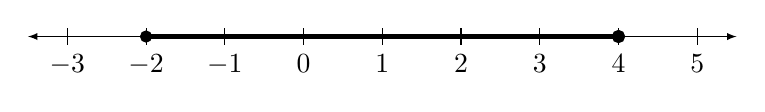
\begin{tikzpicture}
\draw[ultra thick] (-2,0) -- (4,0);
\path [draw=black, fill=black] (-2,0) circle (2pt);
\path [draw=black, fill=black, thick] (4,0.0) circle (2pt);
\draw[latex-latex, very thin] (-3.5,0) -- (5.5,0) ;
\foreach \x in  {-3,-2,-1,0,1,2,3,4,5}
\draw[shift={(\x,0)},color=black] (0pt,3pt) -- (0pt,-3pt);
\foreach \x in {-3,-2,-1,0,1,2,3,4,5}
\draw[shift={(\x,0)},color=black] (0pt,0pt) -- (0pt,-3pt) node[below] 
{$\x$};
\end{tikzpicture}}\\
    \subfloat[]{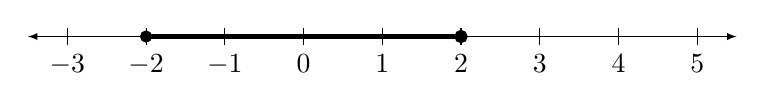
\begin{tikzpicture}
\draw[ultra thick] (-2,0) -- (2,0);
\path [draw=black, fill=black] (-2,0) circle (2pt);
\path [draw=black, fill=black, thick] (2,0.0) circle (2pt);
\draw[latex-latex, very thin] (-3.5,0) -- (5.5,0) ;
\foreach \x in  {-3,-2,-1,0,1,2,3,4,5}
\draw[shift={(\x,0)},color=black] (0pt,3pt) -- (0pt,-3pt);
\foreach \x in {-3,-2,-1,0,1,2,3,4,5}
\draw[shift={(\x,0)},color=black] (0pt,0pt) -- (0pt,-3pt) node[below] 
{$\x$};
\end{tikzpicture}}\\
    \subfloat[]{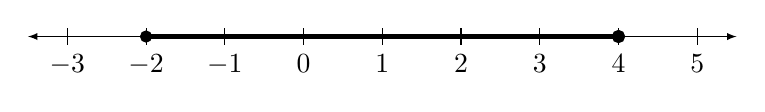
\begin{tikzpicture}
\draw[ultra thick] (-2,0) -- (4,0);
\path [draw=black, fill=black] (-2,0) circle (2pt);
\path [draw=black, fill=black, thick] (4,0.0) circle (2pt);
\draw[latex-latex, very thin] (-3.5,0) -- (5.5,0) ;
\foreach \x in  {-3,-2,-1,0,1,2,3,4,5}
\draw[shift={(\x,0)},color=black] (0pt,3pt) -- (0pt,-3pt);
\foreach \x in {-3,-2,-1,0,1,2,3,4,5}
\draw[shift={(\x,0)},color=black] (0pt,0pt) -- (0pt,-3pt) node[below] 
{$\x$};
\end{tikzpicture}}\\
%\caption{}
\label{fig:fig_p3}
\end{figure}
$$\blacklozenge$$
\newpage
\section{Some remarks on the use of the connectives \textit{and, or, implies}}
\subsection{}
\begin{tcolorbox}
Demonstrate by means of a table showing truth values that the following is a true statement for any choice of $p$ and $q$. Thus show that it is a tautology.
$$(\lnot q\Rightarrow \lnot p)\Rightarrow ( p \Rightarrow q)$$
\end{tcolorbox}
\begin{displaymath}
\begin{array}{|c c|c c|c|c|c|}
% |c c|c| means that there are three columns in the table and
% a vertical bar ’|’ will be printed on the left and right borders,
% and between the second and the third columns.
% The letter ’c’ means the value will be centered within the column,
% letter ’l’, left-aligned, and ’r’, right-aligned.
p & q &\lnot q &\lnot p &\lnot q\Rightarrow \lnot p& p\Rightarrow q&(\lnot q\Rightarrow \lnot p)\Rightarrow ( p \Rightarrow q) \\ % Use & to separate the columns
\hline % Put a horizontal line between the table header and the rest.
T & T &F&F& T&T&T\\
T & F &T&F& F&F&T\\
F & T &F&T& T&T&T\\
F & F &T&T& T&T&T\\
\end{array}
\end{displaymath}
$$\blacklozenge$$

\subsection{}
\begin{tcolorbox}
Show by means of a truth table  that the statement 
$$((p\Rightarrow q) \wedge (q\Rightarrow r))\Rightarrow (p\Rightarrow r)$$
is a tautology.
\end{tcolorbox}
\begin{displaymath}
\begin{array}{|c c c|c| c|c|c|c|}
p & q &r & p\Rightarrow q &q\Rightarrow r &(p\Rightarrow q) \wedge (q\Rightarrow r))& p\Rightarrow r&((p\Rightarrow q) \wedge (q\Rightarrow r))\Rightarrow (p\Rightarrow r)\\ % 
\hline 
T & T &T&T&T& T&T&T\\
T & T &F&T&F& F&F&T\\
T & F &T&F&T& F&T&T\\
T & F &F&F&T& F&F&T\\
F & T &T&T&T& T&T&T\\
F & T &F&T&F& F&T&T\\
F & F &T&T&T& T&T&T\\
F & F &F&T&T& T&T&T\\
\end{array}
\end{displaymath}
$$\blacklozenge$$
\subsection{}
\begin{tcolorbox}
Show by means of a truth table  that  
$$(p\wedge q) \Rightarrow (p\vee q)$$
is a tautology.
\end{tcolorbox}
\begin{displaymath}
\begin{array}{|c c|c|c|c|}
p & q &p\wedge q& p\vee q&(p\wedge q) \Rightarrow (p\vee q) \\ 
\hline 
T & T & T&T&T\\
T & F & F&F&T\\
F & T & F&T&T\\
F & F & F&F&T\\
\end{array}
\end{displaymath}
$$\blacklozenge$$
\subsection{}
\begin{tcolorbox}
Suppose that $p$ and $q$ are statements such that $(p \wedge q)$ is a false statement. Does it follow that the statement
$$(p\text{ is false}) \vee (q\text{ is false})$$is a true statement?
\end{tcolorbox}
\begin{displaymath}
\begin{array}{|c c|c|c c| c|}
p & q &p\wedge q& \lnot p&\lnot q& \lnot p \vee \lnot q\\ % Use & to separate the columns
\hline % Put a horizontal line between the table header and the rest.
T & F & F&F&T&T\\
F & T & F&T&F&T\\
F & F & F&T&T&T\\
\end{array}
\end{displaymath}
\textbf{The answer is Yes}.
$$\blacklozenge$$

\subsection{}
\begin{tcolorbox}
Negate the following statement: \textit{If two angles of a triangle have equal measure, then the length of two sides of that triangle are equal.}
\end{tcolorbox}
First we note that $\lnot(p\Rightarrow q)\Leftrightarrow (p \wedge \lnot q)$. Indeed,

\begin{displaymath}
\begin{array}{|c c|c|c | c|c| c|}

p & q &p\Rightarrow q& \lnot(p\Rightarrow q)&\lnot q&p \wedge \lnot q &\lnot(p\Rightarrow q)\Leftrightarrow (p \wedge \lnot q)\\ % Use & to separate the columns
\hline % Put a horizontal line between the table header and the rest.
T & T & T&F&F&F&T\\
T & F & F&T&T&T&T\\
F & T & T&F&F&F&T\\
F & F & T&F&T&F&T\\
\end{array}
\end{displaymath}
Putting $p$ as \textit{two angles of a triangle have equal measure} and $\lnot q$ as \textit{no two sides of that triangle have equal length} we get the true 'false' statement:\\
\textbf{Two angles of a triangle have equal measure} $\wedge$  \textbf{no two sides of that triangle have equal length}. 
$$\blacklozenge$$

\subsection{}
\begin{tcolorbox}
Write the contrapositive of the statement in Exercise 5.
\end{tcolorbox}
The contrapositive of $p\Rightarrow q$ is $\lnot q\Rightarrow \lnot p$.
Putting $\lnot p$ as \textit{no two angles of a triangle have equal measure} and $\lnot q$ as \textit{no two sides of that triangle have equal length} we get \\
\textbf{If no two sides of that triangle have equal length then no two angles of a triangle have equal measure.}
$$\blacklozenge$$

\subsection{}
\begin{tcolorbox}
Write the converse of the statement in Exercise 5.
\end{tcolorbox}
The converse of $p\Rightarrow q$ is $q\Rightarrow  p$,  giving \\
\textbf{If two sides of a triangle have equal length then  two angles of a that triangle have equal measure.}
$$\blacklozenge$$

\subsection{}
\begin{tcolorbox}
Write the contrapositive of the following statement\\
\textit{If a person belongs to Committee A, then he must be a member of Committee B and he must be a member of Committee C.}
\end{tcolorbox}
Lets put 
\begin{align*}
p\equiv \text{a person belongs to Committee A}\\
q\equiv \text{a person belongs to Committee B}\\
r\equiv \text{a person belongs to Committee C}\\
\end{align*}
then the given statement translates as 
$$p\Rightarrow (q\wedge r)$$

and the contrapositive 
$$\lnot (q\wedge r)\Rightarrow \lnot p$$
This last statement is equivalent with 
$$(\lnot q\vee \lnot r)\Rightarrow \lnot p$$ or in plain text:\\
\textbf{If a person does not belong to Committee B or C , then he is not  a member of Committee A.}
$$\blacklozenge$$

\subsection{}
\begin{tcolorbox}
Write the contrapositive of the following statement\\
$$\text{If } x\in A \text{ and } x\in B\text{, then } x \in C$$
\end{tcolorbox}
Lets put 
\begin{align*}
p\equiv x\in A\\
q\equiv x\in B\\
r\equiv x\in C\\
\end{align*}
then the given statement translates as 
$$p\wedge r\Rightarrow r$$

and the contrapositive 
$$\lnot (r)\Rightarrow \lnot (p\wedge q)$$
This last statement is equivalent with 
$$\lnot (r)\Rightarrow (\lnot p\vee \lnot q)$$ i.e:\\
$$x\notin C \Rightarrow (x\notin A \vee x\notin B)$$
$$\blacklozenge$$
\newpage
\section{Subsets}
No exercises!
\section{Union and Intersection of sets}
\subsection{}
\begin{tcolorbox}
Let $G_1$ be the graph of the equation $x^2+y^2=16$, and let $G_2$ be the graph of the equation $x^2-y^2=1$. Sketch the sets $G_1\cup G_2$ and $G_1\cap G_2$.
\end{tcolorbox}
\begin{figure}[H]%
    \centering
\begin{tikzpicture}
\begin{axis}[ 
xlabel=$x$,
ylabel=$y$,
axis x line=center, xlabel style={anchor=north west},
axis y line=center, ylabel style={anchor=south west},
xmin=-4.5,
xmax=4.5,
ymin=-5.5,
ymax=5.5,
axis line style={thick, shorten > = -0.5cm, shorten < = -0.5cm},
samples=50,
unit vector ratio*=1 1,
]

\addplot [domain=-4:4, thick, black, smooth]{sqrt(16-x^2)};
\addplot [domain=-4:4, thick, black, smooth]{-sqrt(16-x^2)};
\addplot [domain=-4:-1, thick, black, smooth,<-,>=latex]{sqrt(x^2-1)};
\addplot [domain=-4:-1, thick, black, smooth,,<-,>=latex]{-sqrt(x^2-1)};    
\addplot [domain=1:4, thick, black, smooth,->,>=latex]{sqrt(x^2-1)};
\addplot [domain=1:4, thick, black, smooth,->,>=latex]{-sqrt(x^2-1)};
\coordinate (A) at (axis cs:2.91547,2.7386) {};
\coordinate (B) at (axis cs:+2.91547,-2.7386) {};
\coordinate (C) at (axis cs:-2.91547,2.7386) {};
\coordinate (D) at (axis cs:-2.91547,-2.7386) {};
\draw [fill=white] (A) circle [radius=10.05];
\draw [fill= white] (B) circle [radius=10.05];
\draw [fill= white] (C) circle [radius=10.05];
\draw [fill= white] (D) circle [radius=10.05];
\node[anchor=south ] at (A) {A};
\node[anchor=north ] at (B) {B};
\node[anchor=south ] at (C) {D};
\node[anchor=north ] at (D) {C};

\end{axis};
\coordinate (S) at (3,5.5) {};
\node[anchor=north west] at (S) {$G_1\cap G_2\equiv \{A,B,C,D\}$};
%\path (current axis.south west) +(-0.5cm,-0.5cm) (current axis.north east) +(0.5cm,0.5cm);


\end{tikzpicture}\\
%\caption{}
\label{fig:fig_p8a}
\end{figure}
$G_1\cup G_2$ contains all the points defined by the graphs $G_1$ and $G_2$. 
$G_1\cap G_2\equiv \{A,B,C,D\}$ contains the 4 points at the intersection of the two graphs.
$$\blacklozenge$$
\newpage
\subsection{}
\begin{tcolorbox}
We define the sets $A,\, B,\,C$ as follows: $A=\{(x,y):x^2+y^2\le 9\}$, $ B=\{(x,y):x+y\ge 3\}$, $C=\{(x,y):x\ge 0\}$.\\Draw sketches of each of the following sets:
\begin{align*}
\begin{array}{ll}
(a)&A\cup (B\cup C)\\
(b)&A\cap (B\cup C)\\
(c)&(A\cap B)\cup (A\cap C)\\
(d)&(A\cup B)\cup C\\
(e)&A\cup (B\cap C)\\
(f)&(A\cup B)\cap (A\cup C)\\
\end{array}
\end{align*}
\end{tcolorbox}
\begin{figure}[H]%
    \centering
    \begin{tikzpicture}
\begin{axis}[ 
xlabel=$x$,
ylabel=$y$,
axis x line=center, xlabel style={anchor=north west},
axis y line=center, ylabel style={anchor=south west},
xmin=-4.5,
xmax=5.9,
ymin=-5.5,
ymax=5.5,
axis line style={thick, shorten > = -0.5cm, shorten < = -0.5cm},
samples=50,
unit vector ratio*=1 1,
]

\addplot [domain=-3:3, thick, black, smooth,pattern={Lines[
                  distance=2mm,
                  angle=-45
                 ]},
        pattern color=gray!50]{sqrt(9-x^2)};
\addplot [domain=-3:3, thick, black, smooth,pattern={Lines[
                  distance=2mm,
                  angle=-45
                 ]},
        pattern color=gray!50]{-sqrt(9-x^2)};
\addplot [domain=-5:5, thick, black, smooth,<-,>=latex]{3-x};

\coordinate (A) at (axis cs:5,-2) {};
\coordinate (B) at (axis cs:-4,7) {};
\coordinate (C) at (axis cs:-4,9) {};
\coordinate (D) at (axis cs:5,9) {};
\path[ pattern={Lines[
                  distance=2mm,
                  angle=45
                 ]},
        pattern color=gray!50](A)--(B)--(C)--(D);
\path[ pattern={Lines[
                  distance=2mm,
                  angle=0
                 ]},
        pattern color=gray!50] (axis cs:0,-6) --(axis cs:3,-6)--(axis cs:3,6)--(axis cs:0,6)--(axis cs:0,6);
%\node[anchor=south ] at (A) {A};
\begin{scope}
\coordinate (S) at (axis cs:-1.5,1.5) {};
\coordinate (St) at (axis cs:-3.3,3.5) {};
\draw [fill= white] (S) circle [radius=10.05];
\node[above] at (St) {$A$};
\draw[-{Latex[length=2mm]}] (St) .. controls ([xshift=-1cm] S) and ( S) .. (S);

\coordinate (P) at (axis cs:2,-4) {};
\coordinate (Pt) at (axis cs:4,-3.5) {};
\draw [fill= white] (P) circle [radius=10.05];
\node[above] at (Pt) {$C$};
\draw[-{Latex[length=2mm]}] (Pt) .. controls ([xshift=-0.5cm] Pt) and ( P) .. (P);


\coordinate (T) at (axis cs:4,1.5) {};
\coordinate (Tt) at (axis cs:5.5,3.5) {};
\draw [fill= white] (T) circle [radius=10.05];
\node[above] at (Tt) {$B$};
\draw[-{Latex[length=2mm]}] (Tt) .. controls ([xshift=1cm] T) and ( T) .. (T);

\end{scope}
\end{axis};
\end{tikzpicture}
\caption{The 3 sets $A,\,B,\, C$}
\label{fig:fig_p8b}
\end{figure}
\begin{figure}[H]%
    \centering
    \subfloat[$A\cup (B\cup C)$ ]{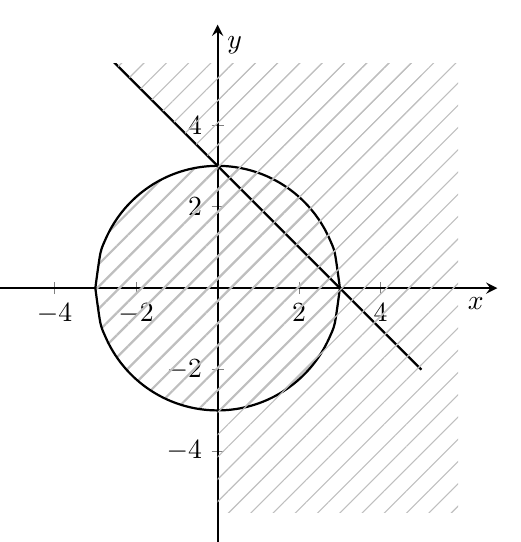
\begin{tikzpicture}
\begin{axis}[ 
xlabel=$x$,
ylabel=$y$,
axis x line=center, xlabel style={anchor=north west},
axis y line=center, ylabel style={anchor=south west},
xmin=-4.5,
xmax=5.9,
ymin=-5.5,
ymax=5.5,
axis line style={thick, shorten > = -0.5cm, shorten < = -0.5cm},
samples=50,
unit vector ratio*=1 1,
]

\addplot [domain=-3:3, thick, black, smooth,pattern={Lines[
                  distance=2mm,
                  angle=45
                 ]},
        pattern color=gray!50]{sqrt(9-x^2)};
\addplot [domain=-3:3, thick, black, smooth,pattern={Lines[
                  distance=2mm,
                  angle=45
                 ]},
        pattern color=gray!50]{-sqrt(9-x^2)};
\addplot [domain=-5:5, thick, black, smooth,<-,>=latex]{3-x};

\coordinate (A) at (axis cs:5,-2) {};
\coordinate (B) at (axis cs:-4,7) {};
\coordinate (C) at (axis cs:-4,9) {};
\coordinate (D) at (axis cs:5,9) {};
\path[ pattern={Lines[
                  distance=2mm,
                  angle=45
                 ]},
        pattern color=gray!50](A)--(B)--(C)--(D);
\path[ pattern={Lines[
                  distance=2mm,
                  angle=45
                 ]},
        pattern color=gray!50] (axis cs:0,-6) --(axis cs:6,-6)--(axis cs:6,6)--(axis cs:0,6)--(axis cs:0,6);

\end{axis};
\end{tikzpicture}}
    \subfloat[$A\cap (B\cup C)$]{\begin{tikzpicture}
\begin{axis}[
xlabel=$x$,
ylabel=$y$,
axis x line=center, xlabel style={anchor=north west},
axis y line=center, ylabel style={anchor=south west},
xmin=-4.5,
xmax=5.9,
ymin=-5.5,
ymax=5.5,
axis line style={thick, shorten > = -0.5cm, shorten < = -0.5cm},
samples=50,
unit vector ratio*=1 1,
]

\addplot [domain=-3:3, thick, black, smooth]{sqrt(9-x^2)};
\addplot [domain=-3:3, thick, black, smooth]{-sqrt(9-x^2)};
\addplot [domain=0:3, thick, black, smooth,pattern={Lines[
                  distance=2mm,
                  angle=45
                 ]},
        pattern color=gray!50]{sqrt(9-x^2)};
\addplot [domain=-0:3, thick, black, smooth,pattern={Lines[
                  distance=2mm,
                  angle=45
                 ]},
        pattern color=gray!50]{-sqrt(9-x^2)};
\addplot [domain=-5:5, thick, black, smooth]{3-x};
% Draw semicircle
\fill[pattern={Lines[
                  distance=2mm,
                  angle=45
                 ]},
        pattern color=gray!50]  (axis cs:3,0) arc (0:-90:300) |- cycle;
\fill[pattern={Lines[
                  distance=2mm,
                  angle=45
                 ]},
        pattern color=gray!50]  (axis cs:3,0) arc (0:90:300) |- cycle;
\end{axis};
\end{tikzpicture}}\\
    \subfloat[$(A\cap B)\cup (A\cap C)$]{\begin{tikzpicture}
\begin{axis}[
xlabel=$x$,
ylabel=$y$,
axis x line=center, xlabel style={anchor=north west},
axis y line=center, ylabel style={anchor=south west},
xmin=-4.5,
xmax=5.9,
ymin=-5.5,
ymax=5.5,
axis line style={thick, shorten > = -0.5cm, shorten < = -0.5cm},
samples=50,
unit vector ratio*=1 1,
]

\addplot [domain=-3:3, thick, black, smooth]{sqrt(9-x^2)};
\addplot [domain=-3:3, thick, black, smooth]{-sqrt(9-x^2)};
\addplot [domain=0:3, thick, black, smooth,pattern={Lines[
                  distance=2mm,
                  angle=45
                 ]},
        pattern color=gray!50]{sqrt(9-x^2)};
\addplot [domain=-0:3, thick, black, smooth,pattern={Lines[
                  distance=2mm,
                  angle=45
                 ]},
        pattern color=gray!50]{-sqrt(9-x^2)};
\addplot [domain=-5:5, thick, black, smooth]{3-x};
% Draw semicircle
\fill[pattern={Lines[
                  distance=2mm,
                  angle=45
                 ]},
        pattern color=gray!50]  (axis cs:3,0) arc (0:-90:300) |- cycle;
\fill[pattern={Lines[
                  distance=2mm,
                  angle=45
                 ]},
        pattern color=gray!50]  (axis cs:3,0) arc (0:90:300) |- cycle;
\end{axis};
\end{tikzpicture}}
    \subfloat[$(A\cup B)\cup C$]{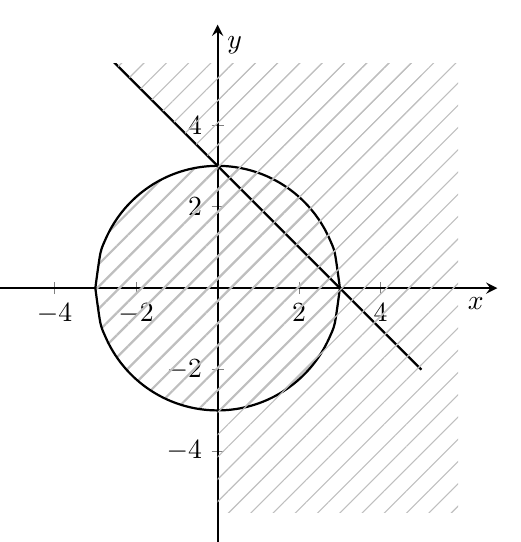
\begin{tikzpicture}
\begin{axis}[ 
xlabel=$x$,
ylabel=$y$,
axis x line=center, xlabel style={anchor=north west},
axis y line=center, ylabel style={anchor=south west},
xmin=-4.5,
xmax=5.9,
ymin=-5.5,
ymax=5.5,
axis line style={thick, shorten > = -0.5cm, shorten < = -0.5cm},
samples=50,
unit vector ratio*=1 1,
]

\addplot [domain=-3:3, thick, black, smooth,pattern={Lines[
                  distance=2mm,
                  angle=45
                 ]},
        pattern color=gray!50]{sqrt(9-x^2)};
\addplot [domain=-3:3, thick, black, smooth,pattern={Lines[
                  distance=2mm,
                  angle=45
                 ]},
        pattern color=gray!50]{-sqrt(9-x^2)};
\addplot [domain=-5:5, thick, black, smooth,<-,>=latex]{3-x};

\coordinate (A) at (axis cs:5,-2) {};
\coordinate (B) at (axis cs:-4,7) {};
\coordinate (C) at (axis cs:-4,9) {};
\coordinate (D) at (axis cs:5,9) {};
\path[ pattern={Lines[
                  distance=2mm,
                  angle=45
                 ]},
        pattern color=gray!50](A)--(B)--(C)--(D);
\path[ pattern={Lines[
                  distance=2mm,
                  angle=45
                 ]},
        pattern color=gray!50] (axis cs:0,-6) --(axis cs:6,-6)--(axis cs:6,6)--(axis cs:0,6)--(axis cs:0,6);

\end{axis};
\end{tikzpicture}}\\
    \subfloat[$A\cup (B\cap C)$]{\begin{tikzpicture}
\begin{axis}[
xlabel=$x$,
ylabel=$y$,
axis x line=center, xlabel style={anchor=north west},
axis y line=center, ylabel style={anchor=south west},
xmin=-4.5,
xmax=5.9,
ymin=-5.5,
ymax=5.5,
axis line style={thick, shorten > = -0.5cm, shorten < = -0.5cm},
samples=50,
unit vector ratio*=1 1,
]

\addplot [domain=-3:3, thick, black, smooth,,pattern={Lines[
                  distance=2mm,
                  angle=45
                 ]},
        pattern color=gray!50]{sqrt(9-x^2)};
\addplot [domain=-3:3, thick, black, smooth,,pattern={Lines[
                  distance=2mm,
                  angle=45
                 ]},
        pattern color=gray!50]{-sqrt(9-x^2)};
\addplot [domain=0:3, thick, black, smooth,pattern={Lines[
                  distance=2mm,
                  angle=45
                 ]},
        pattern color=gray!50]{sqrt(9-x^2)};
\addplot [domain=-0:3, thick, black, smooth,pattern={Lines[
                  distance=2mm,
                  angle=45
                 ]},
        pattern color=gray!50]{-sqrt(9-x^2)};
\addplot [domain=-5:5, thick, black, smooth]{3-x};
% Draw semicircle
\fill[pattern={Lines[
                  distance=2mm,
                  angle=45
                 ]},
        pattern color=gray!50]  (axis cs:3,0) arc (0:-90:300) |- cycle;
\fill[pattern={Lines[
                  distance=2mm,
                  angle=45
                 ]},
        pattern color=gray!50]  (axis cs:0,3)--(axis cs:5,-2)--(axis cs:5,6)--(axis cs:0,6);
\end{axis};
\end{tikzpicture}}
    \subfloat[$(A\cup B)\cap (A\cup C)$]{\begin{tikzpicture}
\begin{axis}[
xlabel=$x$,
ylabel=$y$,
axis x line=center, xlabel style={anchor=north west},
axis y line=center, ylabel style={anchor=south west},
xmin=-4.5,
xmax=5.9,
ymin=-5.5,
ymax=5.5,
axis line style={thick, shorten > = -0.5cm, shorten < = -0.5cm},
samples=50,
unit vector ratio*=1 1,
]

\addplot [domain=-3:3, thick, black, smooth,,pattern={Lines[
                  distance=2mm,
                  angle=45
                 ]},
        pattern color=gray!50]{sqrt(9-x^2)};
\addplot [domain=-3:3, thick, black, smooth,,pattern={Lines[
                  distance=2mm,
                  angle=45
                 ]},
        pattern color=gray!50]{-sqrt(9-x^2)};
\addplot [domain=0:3, thick, black, smooth,pattern={Lines[
                  distance=2mm,
                  angle=45
                 ]},
        pattern color=gray!50]{sqrt(9-x^2)};
\addplot [domain=-0:3, thick, black, smooth,pattern={Lines[
                  distance=2mm,
                  angle=45
                 ]},
        pattern color=gray!50]{-sqrt(9-x^2)};
\addplot [domain=-5:5, thick, black, smooth]{3-x};
% Draw semicircle
\fill[pattern={Lines[
                  distance=2mm,
                  angle=45
                 ]},
        pattern color=gray!50]  (axis cs:3,0) arc (0:-90:300) |- cycle;
\fill[pattern={Lines[
                  distance=2mm,
                  angle=45
                 ]},
        pattern color=gray!50]  (axis cs:0,3)--(axis cs:5,-2)--(axis cs:5,6)--(axis cs:0,6);
\end{axis};
\end{tikzpicture}}\\
%\caption{}
\label{fig:fig_p8b}
\end{figure}
$$\blacklozenge$$
\subsection{}
\begin{tcolorbox}
Let $A,\, B,\,C$ as follows: $A=\{(x,y):x+y\le 5\}$, $ B=\{(x,y):x+y\ge 3\}$, $C=\{(x,y):x\ge 3\}$, and $D=\{(x,y):y\ge 3\}$.\\Draw a sketch for each of the following sets:
\begin{align*}
\begin{array}{ll}
(a)&(A\cap B)\cap C\\
(b)&[(A\cap B)\cap C]\cap D
\end{array}
\end{align*}
\end{tcolorbox}
\begin{figure}[H]%
    \centering
    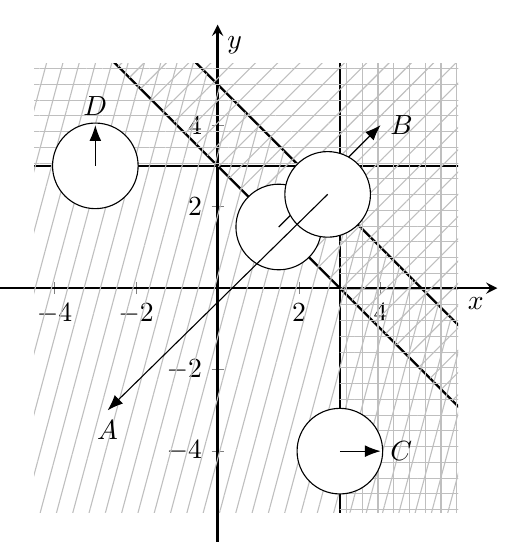
\begin{tikzpicture}
\begin{axis}[ 
xlabel=$x$,
ylabel=$y$,
axis x line=center, xlabel style={anchor=north west},
axis y line=center, ylabel style={anchor=south west},
xmin=-4.5,
xmax=5.9,
ymin=-5.5,
ymax=5.5,
axis line style={thick, shorten > = -0.5cm, shorten < = -0.5cm},
samples=50,
unit vector ratio*=1 1,
]

\addplot [domain=-5:6, thick, black]{3-x};
\addplot [domain=-5:6, thick, black]{5-x};
\draw[thick] (axis cs:3,6)--(axis cs:3,-6){};
\addplot [domain=-6:6, thick, black]{3};

\coordinate (A) at (axis cs:6,-3) {};
\coordinate (B) at (axis cs:-6,9) {};
\coordinate (C) at (axis cs:-6,6) {};
\coordinate (D) at (axis cs:6,9) {};
\path[ pattern={Lines[
                  distance=2mm,
                  angle=45
                 ]},
        pattern color=gray!50](A)--(B)--(C)--(D);
\path[ pattern={Lines[
                  distance=2mm,
                  angle=0
                 ]},
        pattern color=gray!50] (axis cs:3,-6) --(axis cs:3,6)--(axis cs:6,6)--(axis cs:6,-6)--(axis cs:3,-6);


\coordinate (Ab) at (axis cs:6,-1) {};
\coordinate (Bb) at (axis cs:-6,11) {};
\coordinate (Cb) at (axis cs:-6,-6) {};
\coordinate (Db) at (axis cs:6,-6) {};
\path[ pattern={Lines[
                  distance=2mm,
                  angle=75
                 ]},
        pattern color=gray!50](Ab)--(Bb)--(Cb)--(Db);
        
\path[ pattern={Lines[
                  distance=2mm,
                  angle=0
                 ]},
        pattern color=gray!50] (axis cs:3,-6) --(axis cs:3,6)--(axis cs:6,6)--(axis cs:6,-6)--(axis cs:3,-6);

\path[ pattern={Lines[
                  distance=2mm,
                  angle=0
                 ]},
        pattern color=gray!50] (axis cs:-6,3) --(axis cs:6,3)--(axis cs:6,6)--(axis cs:-6,6)--(axis cs:-6,3);
\path[ pattern={Lines[
                  distance=2mm,
                  angle=90
                 ]},
        pattern color=gray!50] (axis cs:3,6) --(axis cs:3,-6)--(axis cs:6,-6)--(axis cs:6,6)--(axis cs:3,6);
%\node[anchor=south ] at (A) {A};
\begin{scope}
\coordinate (S) at (axis cs:1.5,1.5) {};
\coordinate (St) at (axis cs:4,4) {};
\draw [fill= white] (S) circle [radius=1.05];
\node[right] at (St) {$B$};
\draw[-{Latex[length=2mm]}] (S) --(St);

\coordinate (Sd) at (axis cs:-3,3) {};
\coordinate (Std) at (axis cs:-3,4) {};
\draw [fill= white] (Sd) circle [radius=1.05];
\node[above] at (Std) {$D$};
\draw[-{Latex[length=2mm]}] (Sd) --(Std);

\coordinate (P) at (axis cs:3,-4) {};
\coordinate (Pt) at (axis cs:4,-4) {};
\draw [fill= white] (P) circle [radius=1.05];
\node[right] at (Pt) {$C$};
\draw[-{Latex[length=2mm]}] (P) --(Pt);


\coordinate (T) at (axis cs:2.7,2.3) {};
\coordinate (Tt) at (axis cs:-2.7,-3) {};
\draw [fill= white] (T) circle [radius=1.05];
\node[below] at (Tt) {$A$};
\draw[-{Latex[length=2mm]}] (T) --(Tt);

\end{scope}
\end{axis};
\end{tikzpicture}
\caption{The 4 sets $A,\,B,\, C,\, D$}
\label{fig:fig_p8b}
\end{figure}
\begin{figure}[H]%
    \centering
    \subfloat[$(A\cap B)\cap C$ ]{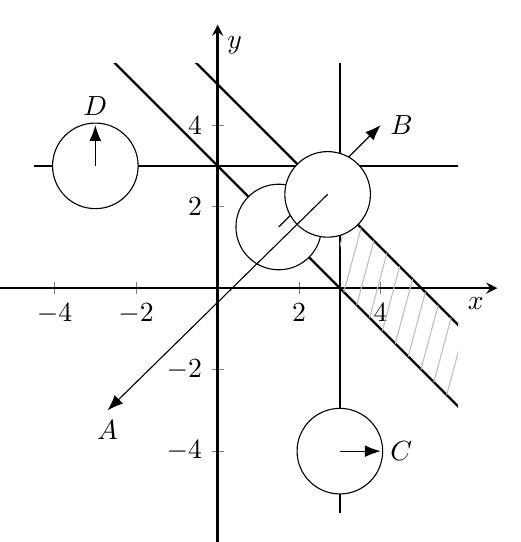
\begin{tikzpicture}
\begin{axis}[ 
xlabel=$x$,
ylabel=$y$,
axis x line=center, xlabel style={anchor=north west},
axis y line=center, ylabel style={anchor=south west},
xmin=-4.5,
xmax=5.9,
ymin=-5.5,
ymax=5.5,
axis line style={thick, shorten > = -0.5cm, shorten < = -0.5cm},
samples=50,
unit vector ratio*=1 1,
]

\addplot [domain=-5:6, thick, black]{3-x};
\addplot [domain=-5:6, thick, black]{5-x};
\draw[thick] (axis cs:3,6)--(axis cs:3,-6){};
\addplot [domain=-6:6, thick, black]{3};

\coordinate (A) at (axis cs:3,0) {};
\coordinate (B) at (axis cs:3,2) {};
\coordinate (C) at (axis cs:6,-1) {};
\coordinate (D) at (axis cs:6,-3) {};


\coordinate (Ab) at (axis cs:6,-1) {};
\coordinate (Bb) at (axis cs:-6,11) {};
\coordinate (Cb) at (axis cs:-6,-6) {};
\coordinate (Db) at (axis cs:6,-6) {};

\path[ pattern={Lines[
                  distance=2mm,
                  angle=75
                 ]},
        pattern color=gray!50](A)--(B)--(C)--(D);
 
\begin{scope}
\coordinate (S) at (axis cs:1.5,1.5) {};
\coordinate (St) at (axis cs:4,4) {};
\draw [fill= white] (S) circle [radius=1.05];
\node[right] at (St) {$B$};
\draw[-{Latex[length=2mm]}] (S) --(St);

\coordinate (Sd) at (axis cs:-3,3) {};
\coordinate (Std) at (axis cs:-3,4) {};
\draw [fill= white] (Sd) circle [radius=1.05];
\node[above] at (Std) {$D$};
\draw[-{Latex[length=2mm]}] (Sd) --(Std);

\coordinate (P) at (axis cs:3,-4) {};
\coordinate (Pt) at (axis cs:4,-4) {};
\draw [fill= white] (P) circle [radius=1.05];
\node[right] at (Pt) {$C$};
\draw[-{Latex[length=2mm]}] (P) --(Pt);


\coordinate (T) at (axis cs:2.7,2.3) {};
\coordinate (Tt) at (axis cs:-2.7,-3) {};
\draw [fill= white] (T) circle [radius=1.05];
\node[below] at (Tt) {$A$};
\draw[-{Latex[length=2mm]}] (T) --(Tt);
\end{scope}
\end{axis};
\end{tikzpicture}}
    \subfloat[$( (A\cap B)\cap C)\cap D =\emptyset$]{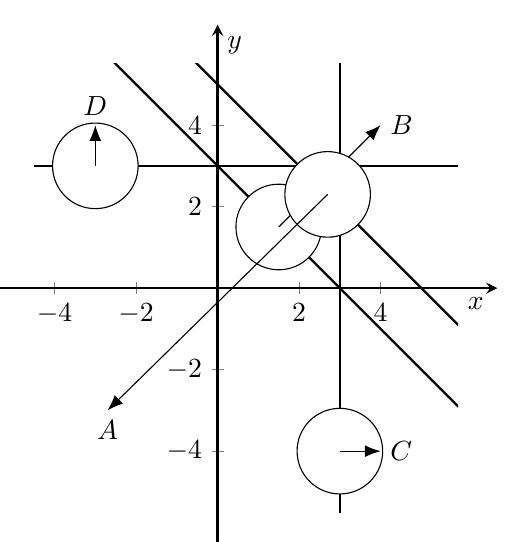
\begin{tikzpicture}
\begin{axis}[ 
xlabel=$x$,
ylabel=$y$,
axis x line=center, xlabel style={anchor=north west},
axis y line=center, ylabel style={anchor=south west},
xmin=-4.5,
xmax=5.9,
ymin=-5.5,
ymax=5.5,
axis line style={thick, shorten > = -0.5cm, shorten < = -0.5cm},
samples=50,
unit vector ratio*=1 1,
]

\addplot [domain=-5:6, thick, black]{3-x};
\addplot [domain=-5:6, thick, black]{5-x};
\draw[thick] (axis cs:3,6)--(axis cs:3,-6){};
\addplot [domain=-6:6, thick, black]{3};

\coordinate (A) at (axis cs:3,0) {};
\coordinate (B) at (axis cs:3,2) {};
\coordinate (C) at (axis cs:6,-1) {};
\coordinate (D) at (axis cs:6,-3) {};


\coordinate (Ab) at (axis cs:6,-1) {};
\coordinate (Bb) at (axis cs:-6,11) {};
\coordinate (Cb) at (axis cs:-6,-6) {};
\coordinate (Db) at (axis cs:6,-6) {};


 
\begin{scope}
\coordinate (S) at (axis cs:1.5,1.5) {};
\coordinate (St) at (axis cs:4,4) {};
\draw [fill= white] (S) circle [radius=1.05];
\node[right] at (St) {$B$};
\draw[-{Latex[length=2mm]}] (S) --(St);

\coordinate (Sd) at (axis cs:-3,3) {};
\coordinate (Std) at (axis cs:-3,4) {};
\draw [fill= white] (Sd) circle [radius=1.05];
\node[above] at (Std) {$D$};
\draw[-{Latex[length=2mm]}] (Sd) --(Std);

\coordinate (P) at (axis cs:3,-4) {};
\coordinate (Pt) at (axis cs:4,-4) {};
\draw [fill= white] (P) circle [radius=1.05];
\node[right] at (Pt) {$C$};
\draw[-{Latex[length=2mm]}] (P) --(Pt);


\coordinate (T) at (axis cs:2.7,2.3) {};
\coordinate (Tt) at (axis cs:-2.7,-3) {};
\draw [fill= white] (T) circle [radius=1.05];
\node[below] at (Tt) {$A$};
\draw[-{Latex[length=2mm]}] (T) --(Tt);
\end{scope}
\end{axis};
\end{tikzpicture}}\\
%\caption{}
\label{fig:fig_p8b}
\end{figure}
$$\blacklozenge$$
\section{Complementation}
\subsection{}
\begin{tcolorbox}
Sketch each of the following sets: (the sets $A,\, B,\, C$ are defined as in exercise $3$page $8$)
\begin{align*}
\begin{array}{ll}
(a)&\sim(A\cap B)\\
(b)&(\sim A)\cup (B)\\
(c)&\sim(A\cup B)\\
(d)&(\sim A)\cap (B)\\
(e)&C - A\\
(f)&\sim(A\cap C)\\
(g)&(\sim A)\cup(\sim B)\\
(h)&(\sim A)\cap (A)\\
(i)&C-(A \cup B)\\
(j)&(C-A)\cap (C-B)\\
(k)&\sim(\sim A)\\
\end{array}
\end{align*}
\end{tcolorbox}
\begin{figure}[H]%
    \centering
    \begin{tikzpicture}
\begin{axis}[ 
xlabel=$x$,
ylabel=$y$,
axis x line=center, xlabel style={anchor=north west},
axis y line=center, ylabel style={anchor=south west},
xmin=-4.5,
xmax=5.9,
ymin=-5.5,
ymax=5.5,
axis line style={thick, shorten > = -0.5cm, shorten < = -0.5cm},
samples=50,
unit vector ratio*=1 1,
]

\addplot [domain=-3:3, thick, black, smooth,pattern={Lines[
                  distance=2mm,
                  angle=-45
                 ]},
        pattern color=gray!50]{sqrt(9-x^2)};
\addplot [domain=-3:3, thick, black, smooth,pattern={Lines[
                  distance=2mm,
                  angle=-45
                 ]},
        pattern color=gray!50]{-sqrt(9-x^2)};
\addplot [domain=-5:5, thick, black, smooth,<-,>=latex]{3-x};

\coordinate (A) at (axis cs:5,-2) {};
\coordinate (B) at (axis cs:-4,7) {};
\coordinate (C) at (axis cs:-4,9) {};
\coordinate (D) at (axis cs:5,9) {};
\path[ pattern={Lines[
                  distance=2mm,
                  angle=45
                 ]},
        pattern color=gray!50](A)--(B)--(C)--(D);
\path[ pattern={Lines[
                  distance=2mm,
                  angle=0
                 ]},
        pattern color=gray!50] (axis cs:0,-6) --(axis cs:3,-6)--(axis cs:3,6)--(axis cs:0,6)--(axis cs:0,6);
%\node[anchor=south ] at (A) {A};
\begin{scope}
\coordinate (S) at (axis cs:-1.5,1.5) {};
\coordinate (St) at (axis cs:-3.3,3.5) {};
\draw [fill= white] (S) circle [radius=10.05];
\node[above] at (St) {$A$};
\draw[-{Latex[length=2mm]}] (St) .. controls ([xshift=-1cm] S) and ( S) .. (S);

\coordinate (P) at (axis cs:2,-4) {};
\coordinate (Pt) at (axis cs:4,-3.5) {};
\draw [fill= white] (P) circle [radius=10.05];
\node[above] at (Pt) {$C$};
\draw[-{Latex[length=2mm]}] (Pt) .. controls ([xshift=-0.5cm] Pt) and ( P) .. (P);


\coordinate (T) at (axis cs:4,1.5) {};
\coordinate (Tt) at (axis cs:5.5,3.5) {};
\draw [fill= white] (T) circle [radius=10.05];
\node[above] at (Tt) {$B$};
\draw[-{Latex[length=2mm]}] (Tt) .. controls ([xshift=1cm] T) and ( T) .. (T);

\end{scope}
\end{axis};
\end{tikzpicture}
\caption{The 3 sets $A,\,B,\, C$}
\label{fig:fig_p8b}
\end{figure}
\begin{figure}[H]%
    \centering
    \subfloat[$\sim(A\cap B)$ ]{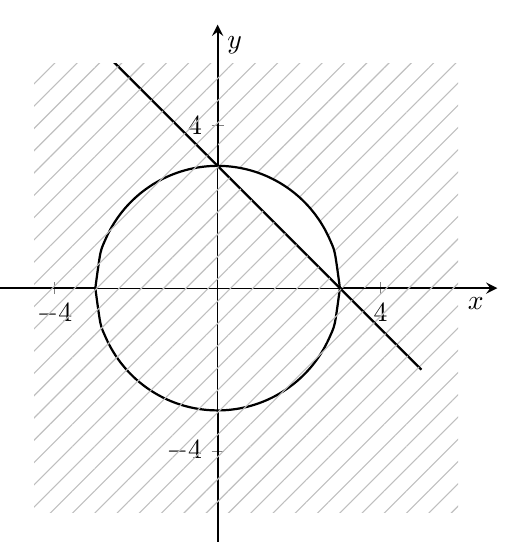
\begin{tikzpicture}
\begin{axis}[ 
xlabel=$x$,
ylabel=$y$,
axis x line=center, xlabel style={anchor=north west},
axis y line=center, ylabel style={anchor=south west},
xmin=-4.5,
xmax=5.9,
ymin=-5.5,
ymax=5.5,
axis line style={thick, shorten > = -0.5cm, shorten < = -0.5cm},
samples=50,
unit vector ratio*=1 1,
]



\coordinate (A) at (axis cs:6,-3) {};
\coordinate (B) at (axis cs:-4,7) {};
\coordinate (C) at (axis cs:-4,9) {};
\coordinate (D) at (axis cs:6,9) {};
\path[ pattern={Lines[
                  distance=2mm,
                  angle=45
                 ]},
        pattern color=gray!50](A)--(B)--(C)--(D);


\addplot [domain=-3:3, thick, black, smooth,fill=white]{sqrt(9-x^2)};
\addplot [domain=-3:3, thick, black, smooth,fill=white]{-sqrt(9-x^2)};
\addplot [domain=-5:5, thick, black, smooth]{3-x};
\draw [](axis cs:-4,0)--(axis cs:4,0);
\draw [](axis cs:0,4)--(axis cs:0,-4);
        \coordinate (At) at (axis cs:-5,8) {};
\coordinate (Bt) at (axis cs:-3,6) {};
\coordinate (Ct) at (axis cs:9,-6) {};
\coordinate (Dt) at (axis cs:-9,-6) {};
\path[ pattern={Lines[
                  distance=2mm,
                  angle=45
                 ]},
        pattern color=gray!50](At)--(Bt)--(Ct)--(Dt);

\end{axis};
\end{tikzpicture}}
    \subfloat[$(\sim A)\cup (B)$]{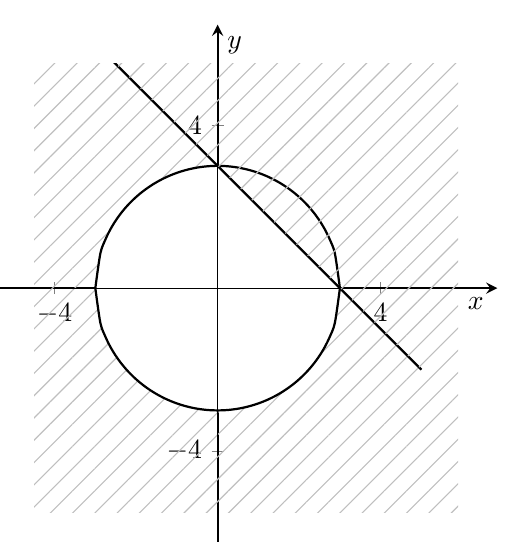
\begin{tikzpicture}
\begin{axis}[ 
xlabel=$x$,
ylabel=$y$,
axis x line=center, xlabel style={anchor=north west},
axis y line=center, ylabel style={anchor=south west},
xmin=-4.5,
xmax=5.9,
ymin=-5.5,
ymax=5.5,
axis line style={thick, shorten > = -0.5cm, shorten < = -0.5cm},
samples=50,
unit vector ratio*=1 1,
]





 \coordinate (At) at (axis cs:-5,8) {};
\coordinate (Bt) at (axis cs:-3,6) {};
\coordinate (Ct) at (axis cs:9,-6) {};
\coordinate (Dt) at (axis cs:-9,-6) {};
\path[ pattern={Lines[
                  distance=2mm,
                  angle=45
                 ]},
        pattern color=gray!50](At)--(Bt)--(Ct)--(Dt);
\addplot [domain=-3:3, thick, black, smooth,fill=white]{sqrt(9-x^2)};
\addplot [domain=-3:3, thick, black, smooth,fill=white]{-sqrt(9-x^2)};
\addplot [domain=-5:5, thick, black, smooth]{3-x};
\draw [](axis cs:-4,0)--(axis cs:4,0);
\draw [](axis cs:0,4)--(axis cs:0,-4);
\coordinate (A) at (axis cs:6,-3) {};
\coordinate (B) at (axis cs:-4,7) {};
\coordinate (C) at (axis cs:-4,9) {};
\coordinate (D) at (axis cs:6,9) {};
\path[ pattern={Lines[
                  distance=2mm,
                  angle=45
                 ]},
        pattern color=gray!50](A)--(B)--(C)--(D);
\end{axis};
\end{tikzpicture}}\\
    \subfloat[$\sim(A\cup B)$]{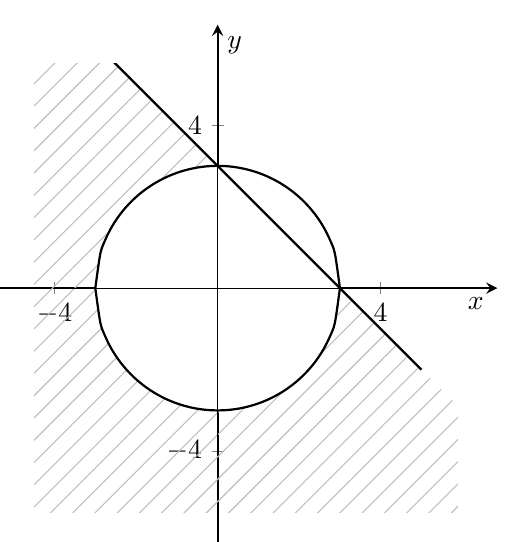
\begin{tikzpicture}
\begin{axis}[ 
xlabel=$x$,
ylabel=$y$,
axis x line=center, xlabel style={anchor=north west},
axis y line=center, ylabel style={anchor=south west},
xmin=-4.5,
xmax=5.9,
ymin=-5.5,
ymax=5.5,
axis line style={thick, shorten > = -0.5cm, shorten < = -0.5cm},
samples=50,
unit vector ratio*=1 1,
]





 \coordinate (At) at (axis cs:-5,8) {};
\coordinate (Bt) at (axis cs:-3,6) {};
\coordinate (Ct) at (axis cs:9,-6) {};
\coordinate (Dt) at (axis cs:-9,-6) {};
\path[ pattern={Lines[
                  distance=2mm,
                  angle=45
                 ]},
        pattern color=gray!50](At)--(Bt)--(Ct)--(Dt);
\addplot [domain=-3:3, thick, black, smooth,fill=white]{sqrt(9-x^2)};
\addplot [domain=-3:3, thick, black, smooth,fill=white]{-sqrt(9-x^2)};
\addplot [domain=-5:5, thick, black, smooth]{3-x};
\draw [](axis cs:-4,0)--(axis cs:4,0);
\draw [](axis cs:0,4)--(axis cs:0,-4);

\end{axis};
\end{tikzpicture}}
    \subfloat[$(\sim A)\cap (B)$]{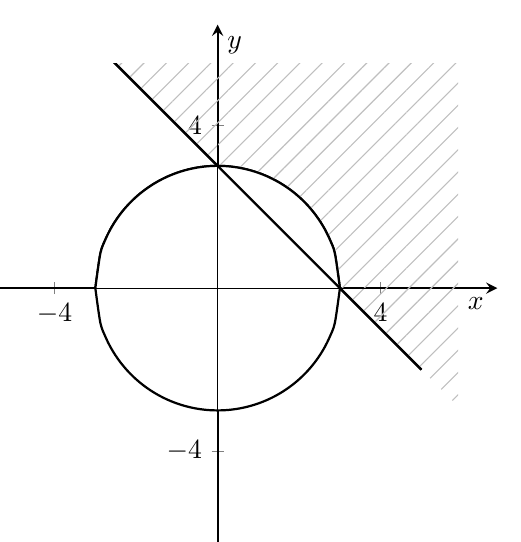
\begin{tikzpicture}
\begin{axis}[ 
xlabel=$x$,
ylabel=$y$,
axis x line=center, xlabel style={anchor=north west},
axis y line=center, ylabel style={anchor=south west},
xmin=-4.5,
xmax=5.9,
ymin=-5.5,
ymax=5.5,
axis line style={thick, shorten > = -0.5cm, shorten < = -0.5cm},
samples=50,
unit vector ratio*=1 1,
]



\addplot [domain=-3:3, thick, black, smooth,fill=white]{sqrt(9-x^2)};
\addplot [domain=-3:3, thick, black, smooth,fill=white]{-sqrt(9-x^2)};
\addplot [domain=-5:5, thick, black, smooth]{3-x};

\coordinate (A) at (axis cs:6,-3) {};
\coordinate (B) at (axis cs:-4,7) {};
\coordinate (C) at (axis cs:-4,9) {};
\coordinate (D) at (axis cs:6,9) {};
\path[ pattern={Lines[
                  distance=2mm,
                  angle=45
                 ]},
        pattern color=gray!50](A)--(B)--(C)--(D);
\addplot [domain=-3:3, thick, black, smooth,fill=white]{sqrt(9-x^2)};
\addplot [domain=-5:5, thick, black, smooth]{3-x};
\draw [](axis cs:-4,0)--(axis cs:4,0);
\draw [](axis cs:0,4)--(axis cs:0,-4);
\end{axis};
\end{tikzpicture}}\\
    \subfloat[$C-A$]{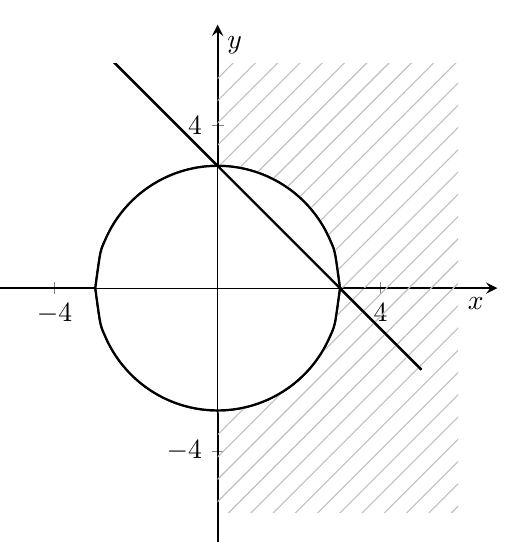
\begin{tikzpicture}
\begin{axis}[ 
xlabel=$x$,
ylabel=$y$,
axis x line=center, xlabel style={anchor=north west},
axis y line=center, ylabel style={anchor=south west},
xmin=-4.5,
xmax=5.9,
ymin=-5.5,
ymax=5.5,
axis line style={thick, shorten > = -0.5cm, shorten < = -0.5cm},
samples=50,
unit vector ratio*=1 1,
]





 \coordinate (At) at (axis cs:-5,8) {};
\coordinate (Bt) at (axis cs:-3,6) {};
\coordinate (Ct) at (axis cs:9,-6) {};
\coordinate (Dt) at (axis cs:-9,-6) {};

\addplot [domain=-3:3, thick, black, smooth,fill=white]{sqrt(9-x^2)};
\addplot [domain=-3:3, thick, black, smooth,fill=white]{-sqrt(9-x^2)};
\addplot [domain=-5:5, thick, black, smooth]{3-x};

\coordinate (A) at (axis cs:6,-3) {};
\coordinate (B) at (axis cs:-4,7) {};
\coordinate (C) at (axis cs:-4,9) {};
\coordinate (D) at (axis cs:6,9) {};

        
        \path[ pattern={Lines[
                  distance=2mm,
                  angle=45
                 ]},
        pattern color=gray!50] (axis cs:0,-6) --(axis cs:6,-6)--(axis cs:36,6)--(axis cs:0,6)--(axis cs:0,6);
\addplot [domain=-3:3, thick, black, smooth,fill=white]{sqrt(9-x^2)};
\addplot [domain=-3:3, thick, black, smooth,fill=white]{-sqrt(9-x^2)};
\addplot [domain=-5:5, thick, black, smooth]{3-x};
\draw [](axis cs:-4,0)--(axis cs:4,0);
\draw [](axis cs:0,4)--(axis cs:0,-4);
\end{axis};
\end{tikzpicture}}
    \subfloat[$ \sim(A\cap C)$]{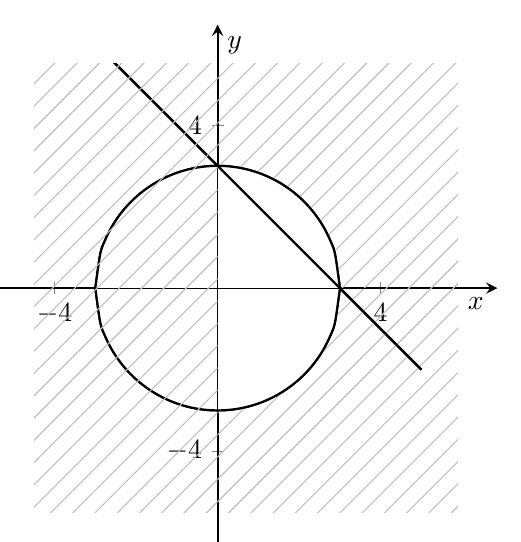
\begin{tikzpicture}
\begin{axis}[ 
xlabel=$x$,
ylabel=$y$,
axis x line=center, xlabel style={anchor=north west},
axis y line=center, ylabel style={anchor=south west},
xmin=-4.5,
xmax=5.9,
ymin=-5.5,
ymax=5.5,
axis line style={thick, shorten > = -0.5cm, shorten < = -0.5cm},
samples=50,
unit vector ratio*=1 1,
]





 \coordinate (At) at (axis cs:-5,8) {};
\coordinate (Bt) at (axis cs:-3,6) {};
\coordinate (Ct) at (axis cs:9,-6) {};
\coordinate (Dt) at (axis cs:-9,-6) {};

\addplot [domain=-3:3, thick, black, smooth,fill=white]{sqrt(9-x^2)};
\addplot [domain=-3:3, thick, black, smooth,fill=white]{-sqrt(9-x^2)};
\addplot [domain=-5:5, thick, black, smooth]{3-x};

\coordinate (A) at (axis cs:6,-3) {};
\coordinate (B) at (axis cs:-4,7) {};
\coordinate (C) at (axis cs:-4,9) {};
\coordinate (D) at (axis cs:6,9) {};

        
        \path[ pattern={Lines[
                  distance=2mm,
                  angle=45
                 ]},
        pattern color=gray!50] (axis cs:0,-6) --(axis cs:6,-6)--(axis cs:6,6)--(axis cs:0,6)--(axis cs:0,6);
\addplot [domain=-3:3, thick, black, smooth,fill=white]{sqrt(9-x^2)};
\addplot [domain=-3:3, thick, black, smooth,fill=white]{-sqrt(9-x^2)};
\addplot [domain=-5:5, thick, black, smooth]{3-x};
\draw [](axis cs:-4,0)--(axis cs:4,0);
\draw [](axis cs:0,4)--(axis cs:0,-4);
        \path[ pattern={Lines[
                  distance=2mm,
                  angle=45
                 ]},
        pattern color=gray!50] (axis cs:0,-6) --(axis cs:-6,-6)--(axis cs:-6,6)--(axis cs:0,6)--(axis cs:0,6);
\end{axis};
\end{tikzpicture}}\\
%\caption{}
\label{fig:fig_p8b}
\end{figure}
\begin{figure}[H]%
    \centering
    \subfloat[$(\sim A)\cup(\sim B)$ ]{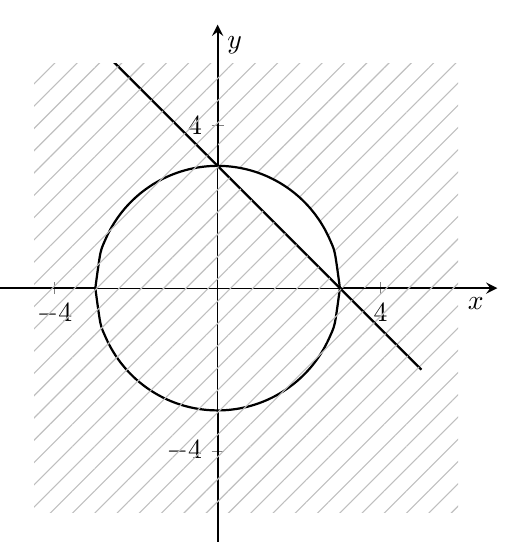
\begin{tikzpicture}
\begin{axis}[ 
xlabel=$x$,
ylabel=$y$,
axis x line=center, xlabel style={anchor=north west},
axis y line=center, ylabel style={anchor=south west},
xmin=-4.5,
xmax=5.9,
ymin=-5.5,
ymax=5.5,
axis line style={thick, shorten > = -0.5cm, shorten < = -0.5cm},
samples=50,
unit vector ratio*=1 1,
]



\coordinate (A) at (axis cs:6,-3) {};
\coordinate (B) at (axis cs:-4,7) {};
\coordinate (C) at (axis cs:-4,9) {};
\coordinate (D) at (axis cs:6,9) {};
\path[ pattern={Lines[
                  distance=2mm,
                  angle=45
                 ]},
        pattern color=gray!50](A)--(B)--(C)--(D);


\addplot [domain=-3:3, thick, black, smooth,fill=white]{sqrt(9-x^2)};
\addplot [domain=-3:3, thick, black, smooth,fill=white]{-sqrt(9-x^2)};
\addplot [domain=-5:5, thick, black, smooth]{3-x};
\draw [](axis cs:-4,0)--(axis cs:4,0);
\draw [](axis cs:0,4)--(axis cs:0,-4);
        \coordinate (At) at (axis cs:-5,8) {};
\coordinate (Bt) at (axis cs:-3,6) {};
\coordinate (Ct) at (axis cs:9,-6) {};
\coordinate (Dt) at (axis cs:-9,-6) {};
\path[ pattern={Lines[
                  distance=2mm,
                  angle=45
                 ]},
        pattern color=gray!50](At)--(Bt)--(Ct)--(Dt);

\end{axis};
\end{tikzpicture}}
    \subfloat[$(\sim A)\cap (A)= \emptyset$]{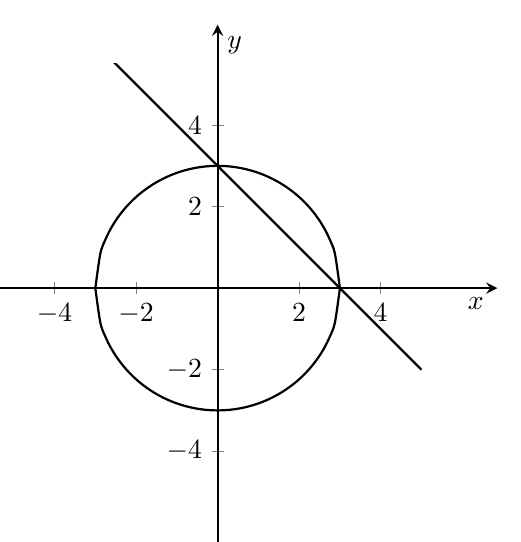
\begin{tikzpicture}
\begin{axis}[ 
xlabel=$x$,
ylabel=$y$,
axis x line=center, xlabel style={anchor=north west},
axis y line=center, ylabel style={anchor=south west},
xmin=-4.5,
xmax=5.9,
ymin=-5.5,
ymax=5.5,
axis line style={thick, shorten > = -0.5cm, shorten < = -0.5cm},
samples=50,
unit vector ratio*=1 1,
]

\addplot [domain=-3:3, thick, black, smooth]{sqrt(9-x^2)};
\addplot [domain=-3:3, thick, black, smooth]{-sqrt(9-x^2)};
\addplot [domain=-5:5, thick, black, smooth,]{3-x};

\end{axis};
\end{tikzpicture}}\\
    \subfloat[$C-(A \cup B) $]{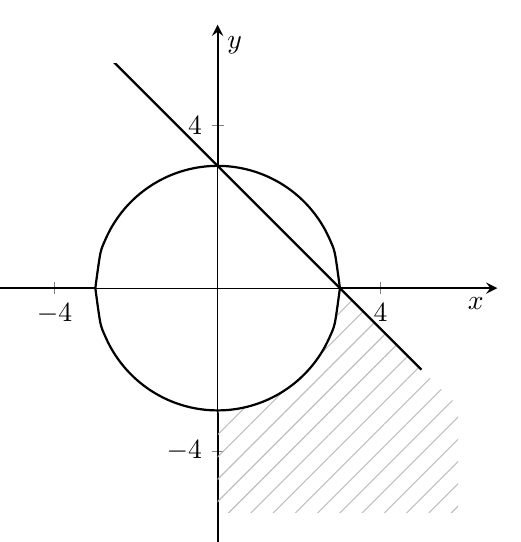
\begin{tikzpicture}
\begin{axis}[ 
xlabel=$x$,
ylabel=$y$,
axis x line=center, xlabel style={anchor=north west},
axis y line=center, ylabel style={anchor=south west},
xmin=-4.5,
xmax=5.9,
ymin=-5.5,
ymax=5.5,
axis line style={thick, shorten > = -0.5cm, shorten < = -0.5cm},
samples=50,
unit vector ratio*=1 1,
]



\coordinate (A) at (axis cs:6,-3) {};
\coordinate (B) at (axis cs:-4,7) {};
\coordinate (C) at (axis cs:-4,9) {};
\coordinate (D) at (axis cs:6,9) {};
       \coordinate (At) at (axis cs:0,0) {};
\coordinate (Bt) at (axis cs:0,-6) {};
\coordinate (Ct) at (axis cs:9,-6) {};
\coordinate (Dt) at (axis cs:0,3) {};
\path[ pattern={Lines[
                  distance=2mm,
                  angle=45
                 ]},
        pattern color=gray!50](At)--(Bt)--(Ct)--(Dt);
\addplot [domain=-3:3, thick, black, smooth,fill=white]{sqrt(9-x^2)};
\addplot [domain=-3:3, thick, black, smooth,fill=white]{-sqrt(9-x^2)};
\addplot [domain=-5:5, thick, black, smooth]{3-x};
\draw [](axis cs:-4,0)--(axis cs:4,0);
\draw [](axis cs:0,4)--(axis cs:0,-4);
\end{axis};
\end{tikzpicture}}
    \subfloat[$(C-A)\cap (C-B)$]{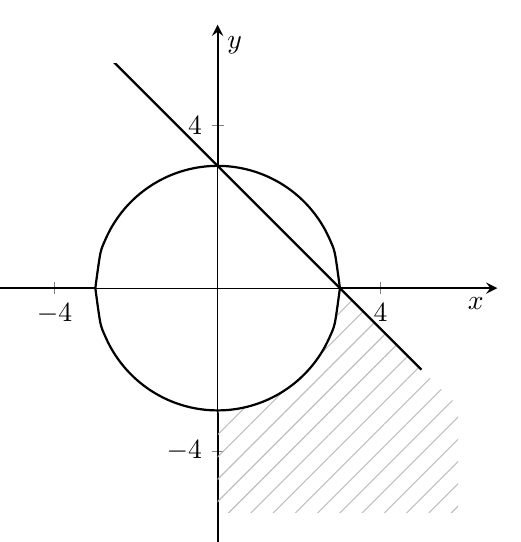
\begin{tikzpicture}
\begin{axis}[ 
xlabel=$x$,
ylabel=$y$,
axis x line=center, xlabel style={anchor=north west},
axis y line=center, ylabel style={anchor=south west},
xmin=-4.5,
xmax=5.9,
ymin=-5.5,
ymax=5.5,
axis line style={thick, shorten > = -0.5cm, shorten < = -0.5cm},
samples=50,
unit vector ratio*=1 1,
]



\coordinate (A) at (axis cs:6,-3) {};
\coordinate (B) at (axis cs:-4,7) {};
\coordinate (C) at (axis cs:-4,9) {};
\coordinate (D) at (axis cs:6,9) {};
       \coordinate (At) at (axis cs:0,0) {};
\coordinate (Bt) at (axis cs:0,-6) {};
\coordinate (Ct) at (axis cs:9,-6) {};
\coordinate (Dt) at (axis cs:0,3) {};
\path[ pattern={Lines[
                  distance=2mm,
                  angle=45
                 ]},
        pattern color=gray!50](At)--(Bt)--(Ct)--(Dt);
\addplot [domain=-3:3, thick, black, smooth,fill=white]{sqrt(9-x^2)};
\addplot [domain=-3:3, thick, black, smooth,fill=white]{-sqrt(9-x^2)};
\addplot [domain=-5:5, thick, black, smooth]{3-x};
\draw [](axis cs:-4,0)--(axis cs:4,0);
\draw [](axis cs:0,4)--(axis cs:0,-4);


\end{axis};
\end{tikzpicture}}\\
    \subfloat[$\sim(\sim A)$]{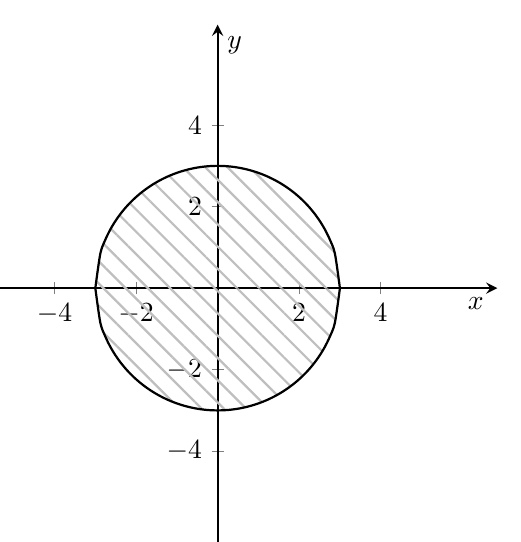
\begin{tikzpicture}
\begin{axis}[ 
xlabel=$x$,
ylabel=$y$,
axis x line=center, xlabel style={anchor=north west},
axis y line=center, ylabel style={anchor=south west},
xmin=-4.5,
xmax=5.9,
ymin=-5.5,
ymax=5.5,
axis line style={thick, shorten > = -0.5cm, shorten < = -0.5cm},
samples=50,
unit vector ratio*=1 1,
]


\addplot [domain=-3:3, thick, black, smooth,pattern={Lines[
                  distance=2mm,
                  angle=-45
                 ]},
        pattern color=gray!50]{sqrt(9-x^2)};
\addplot [domain=-3:3, thick, black, smooth,pattern={Lines[
                  distance=2mm,
                  angle=-45
                 ]},
        pattern color=gray!50]{-sqrt(9-x^2)};
\end{axis}
\end{tikzpicture}}
%\caption{}
\label{fig:fig_p8b}
\end{figure}
$$\blacklozenge$$

\subsection{}
\begin{tcolorbox}
On the basis of the sketches made in the previous exeercise, formulate a proposition about relation that exist concerning complementation, union, and intersection. Try out your conjecture on other examples. In subsequent exercises you will be asked to try to prove such conjectures.
\end{tcolorbox}
\begin{align*}
\begin{array}{ll}
 1.4.2\, (a)\text{ and } (d) &A\cup(B\cup C)= (A\cup B)\cup C)\\
 1.4.2\, (b)\text{ and } (c)& A\cap(B\cup C)= (A\cap B)\cup (A\cap C)\\
 1.4.2(e)\,\text{ and }(f) &A\cup (B\cap C)= (A\cup B)\cap (A\cup C)\\
  1.5.1(a)\,\text{ and }(g) &\sim(A\cap B)=(\sim A)\cup(\sim B)\\
  1.5.1(h)&(\sim A)\cap A=\emptyset\\
  1.5.1(i)\,\text{ and }(j) &C-(A\cup B) = (C-A)\cap (C-B)\\
    1.5.1(k)&\sim (\sim A)=A\\
\end{array}
\end{align*}
$$\blacklozenge$$
\newpage

 \section{Set identities and other set relations}
\subsection{}
\begin{tcolorbox}
Prove that if $A\subset B$, then:
\begin{align*}
\begin{array}{ll}
(a)&A\cap C \subset B \cap C\\
(b)& \sim B \subset \, \sim A\\
(c) &A \cap B = A\\
(d) &A \cup C \subset B\cup C\\
\end{array}
\end{align*}
\end{tcolorbox}
\textbf{a)}$\quad A\cap C \subset B \cap C $\\\\
Given is $x\in B$ if $x \in A$. Suppose $x \in A\cap C$, then $x \in A$ (given) and $x \in C$ but $x \in B$ (given) and as $x \in C$ follows that $x \in B\cap C$. And we conclude that $A\cap C \subset B\cap C$. \\\\
$$\lozenge$$
\textbf{b)}$\quad \sim B \subset \, \sim A$\\\\
Given is $x\in B$ if $x \in A$. If $x\not\in B$ then $x\in \, \sim B$. As $A\subset B$, $x$ will not be in $A$ but $x\in \sim A$. So $x\in \, \sim B \Rightarrow \quad x\in \, \sim A$ and thus $\sim B \subset \, \sim A$. \\\\
$$\lozenge$$

\textbf{c)}$\quad A \cap B = A$\\\\
Given is $x\in B$ if $x \in A$. Suppose $x \in A\cap B$, then $x \in A$ and thus $A\cap B \subset A$. Suppose $x \in A$, then $x \in B$ as $A\subset B$ and thus $x\in A\cap B$ from which we conclude $A \subset A\cap B$.
$$\lozenge$$
\textbf{d)}$\quad A \cup C \subset B\cup C$\\\\
Given is $x\in B$ if $x \in A$. Suppose $x \in A\cup C$, then $x \in A$ or $x\in C$. But $x\in B$ (given), so $x\in B$ or $x\in C$ and thus $x\in B\cup C$, from which we conclude $A\cup C \subset B\cup C$.
$$\blacklozenge$$
\newpage
\subsection{}
\begin{tcolorbox}
Verify that each of the following is an an identity:
\begin{align*}
\begin{array}{ll}
(a)&A\cup \emptyset = A\\
(b)& A\cap \emptyset = \emptyset\\
(c) &A \cap A = A\\
(d) &A \cup A =A\\
(e)&(A\cup B)\cup C= A\cup(B\cup C) \\
(f)& (A\cap B)\cap C= A\cap(B\cap C)\\
(g) &A\cup (B\cap C)= (A\cup B)\cap (A\cup C)\\
(h) &X-(A\cup B) = (X-A)\cap (X-B)\\
(i)&A\, \cap \, \sim A = \emptyset\\
(j)& A\, \cup \, \sim A = U\\
\end{array}
\end{align*}
\end{tcolorbox}
\textbf{a)}$\quad A\cup \emptyset = A $\\\\
This is a consequence of remark 3.3 page 7: the empty set $\emptyset$ is a subset of every set. So, $\emptyset\subset A$ giving the asked identity. \\\\
$$\lozenge$$
\textbf{b)}$\quad A\cap \emptyset = \emptyset$\\\\
If $x\in A\cap \emptyset$ then $x\in \, A$ and $x$ must also be in $\emptyset$ which is impossible by definition. So there is no element $x \in \emptyset$ which can satisfy $x\in A\cap \emptyset$ giving the proposed identity. \\\\
$$\lozenge$$
\textbf{c)}$\quad A \cap A =A$\\\\
 Suppose $x \in A\cap A$, then $x \in A$ and $x\in A$ and thus $x\in A$, giving  $ A \cap A \subset A$. Suppose $x \in A$, then obviously  $x \in A$ and $x \in A$, giving $A\subset A\cap A$. Hence $A \cap A =A$
$$\lozenge$$
\textbf{d)}$\quad A \cup A =A$\\\\
Suppose $x \in A\cup A$, then $x \in A$ or $x\in A$ and thus $x\in A$, giving  $ A \cup A \subset A$. Suppose $x \in A$, then obviously  $x \in A$ or $x \in A$, giving $A\subset A\cup A$. Hence $A \cup A =A$
$$\lozenge$$
\textbf{e)}$\quad (A\cup B)\cup C= A\cup(B\cup C) $\\\\
 Suppose $x \in (A\cup B)\cup C$, then $x \in (A\cup B)$ or $x\in C$ and thus $x\in A$ or $x\in B$ or $x\in C$. So  $x\in B$ or  $x\in C$  can be written as $x\in (B\cup C)$. So $x\in A$ or $x\in (B\cup C)$, giving $(A\cup B)\cup C\subset A\cup(B\cup C)$. The same reasoning yields for $x\in A\cup(B\cup C)$ giving the identity.
$$\lozenge$$
\textbf{f)}$\quad (A\cap B)\cap C= A\cap(B\cap C)$\\\\
 Suppose $x \in (A\cap B)\cap C$, then $x \in (A\cup B)$ and $x\in C$ and thus $x\in A$ and $x\in B$ and $x\in C$. So  $x\in B$ and  $x\in C$  can be written as $x\in (B\cap C)$. So $x\in A$ and $x\in (B\cup C)$, giving $(A\cap B)\cap C\subset A\cap(B\cap C)$. The same reasoning yields for $x\in A\cap(B\cap C)$ giving the identity.
$$\lozenge$$
\textbf{g)}$\quad A\cup (B\cap C)= (A\cup B)\cap (A\cup C)$\\\\
 Suppose $x \in A\cup (B\cap C)$, then $x \in A$ or $x\in (B\cap C)$.  Take the case $x\in A$, then  $x\in A\cup B$ and  $x\in A\cup C$ which implies $x\in (A\cup B)\cap (A\cup C)$, giving $A\cup (B\cap C)\subset (A\cup B)\cap (A\cup C)$. The other case:  if $x\in B\cap C$ then $x\in B$ and $x\in C$. So, $x \in A\cup B$ and $x\in A\cup C$ giving also $A\cup (B\cap C)\subset (A\cup B)\cap (A\cup C)$.\\
 On the other hand,  be $x \in (A\cup B)\cap (A\cup C)$ then $x \in (A\cup B)$  and $x \in (A\cup C)$. Let's first take the case $x\in A$ then obviously $x\in A\cup (B\cap C)$ even if $x\not\in  B\cap C$. Alternatively, be $x\not \in A$ then we must have $x \in B$ and $x\in C$ which implies $x\in B\cap C$, giving again $x\in A\cup (B\cap C)$.
$$\lozenge$$
\textbf{h)}$\quad X-(A\cup B) = (X-A)\cap (X-B)$\\\\
 Suppose $x\in X-(A\cup B)$, then $x \not\in A$ and $x \not\in B$ which implies $x \in X-A$ and $x \in X-B$ and thus $x \in X-A\cap X-B$ giving $X-(A\cup B) \subset (X-A)\cap (X-B)$.\\
 The other way around. Suppose $x\in(X-A)\cap (X-B)$. Then $x\in(X-A)$ and $x\in(X-B)$ which implies  $x\not \in A$ and $x\not \in B$ giving $x\not \in A \cup B$ which in turn implies $x\in X-(A\cup B)$ giving $(X-A)\cap (X-B)\subset  X-(A\cup B)$.\\Conclusion: $ X-(A\cup B) = (X-A)\cap (X-B)$
$$\lozenge$$
\textbf{i)}$\quad A\, \cap \, \sim A = \emptyset$\\\\
 Suppose $x\in A\, \cap \, \sim A$, then $x \in A$ and $x \not\in A$ which is a contradiction, so the only element which is always an element of any set is the empty set, so $ A\, \cap \, \sim A \subset \emptyset$. Suppose on the contrary that $x\in\emptyset$. This implies that $x$ correspond to the empty set and as the empty set is an element of any set, we have  $\emptyset \subset A\, \cap \, \sim A  $
$$\lozenge$$
\textbf{j)}$\quad A\, \cup \, \sim A = U$\\\\
 Suppose $x\in A\, \cup \, \sim A$, then $x \in A$ or $x \not\in A$. So, in any case $x\in U$ and thus $A\, \cup \, \sim A \subset U$.\\
 On the opposite way  suppose that $x\in U$. Then obviously $x\in A$ or $x\in \sim A$ and thus $U\subset A\, \cup \, \sim A$.
$$\blacklozenge$$

\subsection{}
\begin{tcolorbox}
Prove that if $ A\subset C$ and $B\subset C$, then $ A\cup B \subset C$.
\end{tcolorbox}
Given is $A\subset C$ and  $B\subset C$. Take $x\in A$, then $x\in C$, so even if $x\not\in B$, then $x\in A\cup B$ reduces to $x\in A$ and thus $x\in C$. The same reasoning yields for $x\in B$, giving $ A\cup B \subset C$.
$$\blacklozenge$$

\subsection{}
\begin{tcolorbox}
Prove that if $ A\subset B$ and $A\subset C$, then $ A\subset B \cap C$.
\end{tcolorbox}
Given is $A\subset B$ and  $A\subset C$. Take $x\in A$, then $x\in C$ and $x\in B$, which implies $x\in C\cap B$. giving indeed  $ A\subset B \cap C$.
$$\blacklozenge$$
\newpage
 \section{Counterexamples}
 In each of the following exercises state whether the statement is necessarily true. Assume that $A,\, B$ and $C$ are subsets of a universal set $U$. Justify with a proof or a counterexample.
\subsection{}
\begin{tcolorbox}
If $A\cup C=B\cup C$, then $A=B$
\end{tcolorbox}
\textbf{Not TRUE.}\\
\begin{figure}[H]%
    \centering
    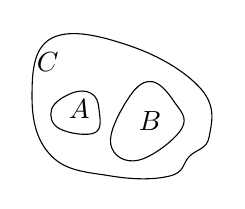
\begin{tikzpicture}[scale=0.5]
\draw  plot[smooth cycle, tension=.7] coordinates {(-5.5,3.8) (-7.5,4) (-8,2.5) (-7.5,1) (-6,0.5) (-4.5,0.5) (-4,1) (-3.5,1.5) (-3.7,2.7)};
\draw  plot[smooth cycle, tension=.7] coordinates {(-7.5,2.2) (-7.3,1.7) (-6.4,1.6) (-6.3,2.2) (-6.5,2.6) (-7,2.6) };
\draw  plot[smooth cycle, tension=.7] coordinates {(-6,1.3) (-5.3,0.9) (-4.2,1.7) (-4.4,2.4) (-5,2.9) (-5.6,2.4) };
\coordinate (C) at (-7.6,2.9) {} {};
\node[above] at (C) {$C$};
\coordinate (A) at (-6.8,1.7) {} {} {};
\node[above] at (A) {$A$};
\coordinate (B) at (-5,1.4) {} {} {};
\node[above] at (B) {$B$};
\end{tikzpicture}
\caption{$A\cup C=B\cup C\not\Rightarrow A=B$}
\label{fig:fig_p8b}
\end{figure}
Be $A\subset C$ and $B\subset C$, then we have $A\cup C=B\cup C\equiv C=C$ even if $A\cap B=\emptyset$.
$$\blacklozenge$$

\subsection{}
\begin{tcolorbox}
$(A\cup B)-B=A$
\end{tcolorbox}
\textbf{Not TRUE.}\\
\begin{figure}[H]%
    \centering
    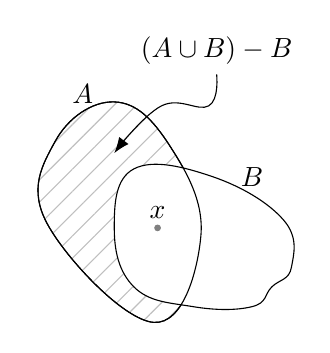
\begin{tikzpicture}[scale=0.5]
\draw[ pattern={Lines[
                  distance=2mm,
                  angle=45
                 ]},
        pattern color=gray!50]  plot[smooth cycle, tension=.7] coordinates {(-9.5,4.7) (-9.7,2.6) (-7,0.1) (-5.8,2.3) (-6.6,4.6) (-8,5.7) };
\draw[ fill = white]  plot[smooth cycle, tension=.7] coordinates {(-5.5,3.8) (-7.5,4) (-8,2.5) (-7.5,1) (-6,0.5) (-4.5,0.5) (-4,1) (-3.5,1.5) (-3.7,2.7)};

\coordinate (C) at (-5.4,6.4) {} {} {} {};
\node[above] at (C) {$(A\cup B)-B$};
\coordinate (A) at (-8.8,5.4) {} {} {} {};
\node[above] at (A) {$A$};
\coordinate (B) at (-4.5,3.3) {} {} {} {};
\node[above] at (B) {$B$};
\draw  plot[smooth cycle, tension=.7] coordinates {(-9.5,4.7) (-9.7,2.6) (-7,0.1) (-5.8,2.3) (-6.6,4.6) (-8,5.7) };

\node (v1) at (-8,4.4) {};
\draw[-{Latex[length=2mm]}] plot[smooth, tension=.7] coordinates {(C) (-5.6,5.6) (-6.8,5.6) (v1)};
\node[above] at (-6.9,2.5) {$x$};
\filldraw [gray] (-6.9,2.5) circle (2pt);: 
\end{tikzpicture}
\caption{$(A\cup B)-B\ne A$ }
\label{fig:fig_p8b}
\end{figure}
Be $A\cap B\neq \emptyset$ , take  $x\in A$ and $x\in B$, then $x$ can't be $x\in (A\cup B)-B$ although it is an element of $A$.
$$\blacklozenge$$

\subsection{}
\begin{tcolorbox}
$(A- B)\cup B=A$
\end{tcolorbox}
\textbf{Not TRUE.}\\
\begin{figure}[H]%
    \centering
    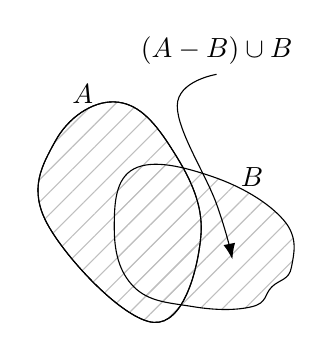
\begin{tikzpicture}[scale=0.5]
\draw[ pattern={Lines[
                  distance=2mm,
                  angle=45
                 ]},
        pattern color=gray!50]  plot[smooth cycle, tension=.7] coordinates {(-9.5,4.7) (-9.7,2.6) (-7,0.1) (-5.8,2.3) (-6.6,4.6) (-8,5.7) };
\draw[ pattern={Lines[
                  distance=2mm,
                  angle=45
                 ]},
        pattern color=gray!50]  plot[smooth cycle, tension=.7] coordinates {(-5.5,3.8) (-7.5,4) (-8,2.5) (-7.5,1) (-6,0.5) (-4.5,0.5) (-4,1) (-3.5,1.5) (-3.7,2.7)};

\coordinate (C) at (-5.4,6.4) {} {} {} {};
\node[above] at (C) {$(A- B)\cup B$};
\coordinate (A) at (-8.8,5.4) {} {} {} {};
\node[above] at (A) {$A$};
\coordinate (B) at (-4.5,3.3) {} {} {} {};
\node[above] at (B) {$B$};
\draw  plot[smooth cycle, tension=.7] coordinates {(-9.5,4.7) (-9.7,2.6) (-7,0.1) (-5.8,2.3) (-6.6,4.6) (-8,5.7) };

\node (v1) at (-5,1.7) {};
\draw[-{Latex[length=2mm]}] plot[smooth, tension=.7] coordinates {(C) (-6.4,5.6) (-5.4,3.1) (v1)};
%\node[above] at (-6.9,2.5) {$x$};
%\filldraw [gray] (-6.9,2.5) circle (2pt);: 
\end{tikzpicture}
\caption{$(A- B)\cup B\ne A$ }
\label{fig:fig_p8b}
\end{figure}
This is only true if $B\subset A$
$$\blacklozenge$$


\subsection{}
\begin{tcolorbox}
$\sim(A-B)=\, \sim(A\, \cap \sim B)$
\end{tcolorbox}
\textbf{ TRUE.}\\

Suppose first that $A$ and $B$ are disjoint, i.e. $A\cap B =\emptyset$, then $A-B=A$ and $\sim (A-B)=\sim A$. On the other hand $A\subset\, \sim B$, so $A\, \cap \sim B=A$, giving $\sim(A\, \cap \sim B)= \sim A$, giving indeed $\sim(A-B)=\sim(A\, \cap \sim B)$.

Suppose now that $A$ and $B$ are not disjoint, i.e. $A\cap B \ne \emptyset$. Be $x\in A-B\subset A$. This is equivalent with the statement $x\in A \wedge x\not\in B$. Negating this statement: $\lnot(x\in A \wedge x\not\in B)\Leftrightarrow x\not\in A \vee x\in B$. This give $\sim(A-B) \equiv  x\not\in A \vee x\in B$.\\
 Be now $x\in A\, \cap \sim B$. This is equivalent with the statement $x\in A \wedge x\not\in B$. Negating this statement: $\lnot(x\in A\, \cap \sim B)\Leftrightarrow x\not\in A \vee x\in B$. This give $\sim(A\, \cap \sim B )\equiv  x\not\in A \vee x\in B$, resulting in $\sim(A-B)=\, \sim(A\, \cap \sim B)$.  
$$\blacklozenge$$


\subsection{}
\begin{tcolorbox}
$\sim(\sim (\sim A)) =\sim A$
\end{tcolorbox}
\textbf{ TRUE.}\\
Be $x\in \,  \sim(\sim (\sim A))$. This is equivalent to $x\not \in  \, \sim (\sim A)$. Which on it's turn is equivalent with $x \in  \, \sim A$. So, $\sim(\sim (\sim A)) \subset\,\sim A$.\\
Be $x\in \,\sim A$. This is equivalent to $x\not \in \, \sim (\sim A)$. Which on it's turn is equivalent with $x \in  \, \sim(\sim (\sim A))$. So, $\sim A \subset\, \sim(\sim (\sim A))$.\\Both cases reduce to $\sim(\sim (\sim A)) =\sim A$.
$$\blacklozenge$$


\subsection{}
\begin{tcolorbox}
$A\cup(B-C)= (A\cup B)-C$
\end{tcolorbox}
\textbf{Not  TRUE.}\\
Be $x\in \,  A\cup(B-C)$. This is equivalent to $x \in  A \vee x \in (B-C) $. Suppose $x\in A$, then $x\in A\cup B$. Let's consider the  set $C$ so that  $(A\cup B) \subset C$, then $(A\cup B) - C=\emptyset$. We get a contradiction and the proposed statement is not true.
$$\blacklozenge$$

\subsection{}
\begin{tcolorbox}
$\sim(A-B)=(\sim A)\cup B$
\end{tcolorbox}
\textbf{TRUE.}\\
Be $x\in (A-B)$. This is equivalent to $x \in  A \wedge x \not\in B $. Negating this statement: $\lnot(x \in  A \wedge x \not\in B )\Leftrightarrow x \not \in  A \vee x \in B $. This is equivalent to the statement $x\in (\sim A)\cup B$. So $\sim(A-B)\subset (\sim A)\cup B$.\\
Consider now $x\in (\sim A)\cup B$. So $x \not \in  A \vee x \in B $. If we have the case $x \not \in  A $ then also $x\not \in (A-B)$ as $x$ can not be one of the remaining elements of $A$ after the complement of $B$ relative to $A$. Also, if  $x \in  B $ then also $x\not \in (A-B)$ as $x$ is an element of $B$ and thus can not be an element of $(A-B)$. Thus, in both cases we have, $x\not \in (A-B)$ which implies $x \in\, \sim (A-B)$. So $ (\sim A)\cup B\subset\sim(A-B)$.\\
$$\blacklozenge$$

\subsection{}
\begin{tcolorbox}
If $A-B=C-B$, then $A=C$.
\end{tcolorbox}
\textbf{Not TRUE.}\\
\begin{figure}[H]%
    \centering
    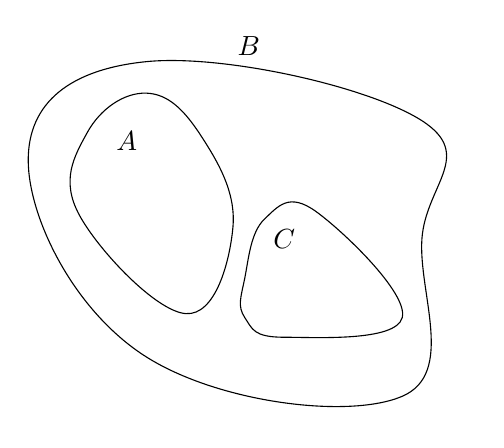
\begin{tikzpicture}[scale=0.5]
\draw[ ]  plot[smooth cycle, tension=.7] coordinates {(-9.5,4.7) (-9.7,2.6) (-7,0.1) (-5.8,2.3) (-6.6,4.6) (-8,5.7) };
\draw[ ]  plot[smooth cycle, tension=.7] coordinates { (-5,2.5) (-5.5,1) (-5.5,0) (-4.5,-0.5) (-1.5,0)   (-3.7,2.7)};

\coordinate (C) at (-5.4,6.4) {} {} {} {};
\node[above] at (C) {$ B$};
\coordinate (A) at (-8.5,4) {} {} {} {} {};
\node[above] at (A) {$A$};
\coordinate (B) at (-4.5,1.5) {} {} {} {} {};
\node[above] at (B) {$C$};
\draw  plot[smooth cycle, tension=.7] coordinates {(-11,4) (-8,-1) (-1.5,-2) (-1,2) (-1,5) (-8,6.5) };
\end{tikzpicture}
\caption{If $A-B=C-B\not\Rightarrow A=C$}
\label{fig:fig_p8b}
\end{figure}
Suppose $A\subset B$, then $A-B=\emptyset$. Choose a $C$ such that $C\subset B$ and also $A\cap C=\emptyset$, then also $C-B=\emptyset$ and get $A-B=C-B$ although $A\ne C$.
$$\blacklozenge$$

\subsection{}
\begin{tcolorbox}
If $A-(B\cap C)=(A-B)\cap (A-C)$.
\end{tcolorbox}
\textbf{TRUE.}\\

Suppose $x\in A-(B\cap C)$, then $x\in A \wedge x\not\in \,B\cap C$. As $x$ can not be simultaneously in $B$ and $C$, then also $x$ must be simultaneously in $A-B$ and $A-C$ as the "complementation of $A$ with $B$ and $C$ will not "subtract" $x$ out of $A$,  and considering that $x\in A$ we have $A-(B\cap C)\subset(A-B)\cap (A-C)$\\
Suppose $x\in (A-B)\cap (A-C)$, then $x$ must be an element of $A$ but not an element of $B$ and $C$. This means that $x\not\in B\cap C$ and thus the complementation of $A$ by $B\cap C$ has no effect on $x$. Thus, $\underbrace{(A-B)\cap (A-C)}_{= A} \subset A-(B\cap C)$.
$$\blacklozenge$$
\newpage
 \section{Collections of Sets}
\subsection{}
\begin{tcolorbox}
Suppose that $A,\, B$ and $C$ are the following subsets of the plane:\\
$A=\{(x,y):x^2+y^2\le 16\},\, B= \{(x,y):x\ge 0 \text{ and } y \le 0\},\, C=\{(x,y): y \le x\}$. If $\mathscr{K}$ is the collection of sets $\{A,\, B,\, C\}$, sketch each of the following sets:

\begin{align*}
\begin{array}{ll}
(a)&\bigcap \mathscr{K}\\
(b)&\bigcup \mathscr{K}\\
(c)&\bigcup \mathscr{K}-\bigcap \mathscr{K}\\
\end{array}
\end{align*}
\end{tcolorbox}
\begin{figure}[H]%
    \centering
    \begin{tikzpicture}
\begin{axis}[ 
xlabel=$x$,
ylabel=$y$,
axis x line=center, xlabel style={anchor=north west},
axis y line=center, ylabel style={anchor=south west},
xmin=-4.5,
xmax=5.9,
ymin=-5.5,
ymax=5.5,
axis line style={thick, shorten > = -0.5cm, shorten < = -0.5cm},
samples=50,
unit vector ratio*=1 1,
]
\addplot [domain=-4:4, thick, black, smooth,pattern={Lines[
                  distance=2mm,
                  angle=-45
                 ]},
        pattern color=gray!50]{sqrt(16-x^2)};
\addplot [domain=-4:4, thick, black, smooth,pattern={Lines[
                  distance=2mm,
                  angle=-45
                 ]},
        pattern color=gray!50]{-sqrt(16-x^2)};
\addplot [domain=-6:6, thick, black]{x};


\coordinate (A) at (axis cs:0,0) {};
\coordinate (B) at (axis cs:6,0) {};
\coordinate (C) at (axis cs:6,-6) {};
\coordinate (D) at (axis cs:0,-6) {};
\path[ pattern={Lines[
                  distance=2mm,
                  angle=90
                 ]},
        pattern color=gray!50](A)--(B)--(C)--(D);

\coordinate (Ab) at (axis cs:-6,-6) {};
\coordinate (Bb) at (axis cs:6,6) {};
\coordinate (Cb) at (axis cs:6,-6) {};
\coordinate (Db) at (axis cs:-6,-6) {};

\path[ pattern={Lines[
                  distance=2mm,
                  angle=45
                 ]},
        pattern color=gray!50](Ab)--(Bb)--(Cb)--(Db);

\begin{scope}

\coordinate (St) at (axis cs:4,-4.5) {};
\draw [fill= white] (St) circle [radius=10.05];
\node[right] at (St) {$B$};



\coordinate (Std) at (axis cs:-3,-4.5) {};
\draw [fill= white] (Std) circle [radius=10.05];
\node[above] at (Std) {$C$};


\coordinate (T) at (axis cs:-2,2.3) {};
\draw [fill= white] (T) circle [radius=10.05];
\node[below] at (T) {$A$};


\end{scope}
\end{axis};
\end{tikzpicture}
\caption{The sets $A,\, B , \, C$}
\label{fig:fig_p8b}
\end{figure}
\textbf{a)} $\bigcap \mathscr{K}$
\begin{figure}[H]%
    \centering
   \begin{tikzpicture}
\begin{axis}[ 
xlabel=$x$,
ylabel=$y$,
axis x line=center, xlabel style={anchor=north west},
axis y line=center, ylabel style={anchor=south west},
xmin=-4.5,
xmax=5.9,
ymin=-5.5,
ymax=5.5,
axis line style={thick, shorten > = -0.5cm, shorten < = -0.5cm},
samples=50,
unit vector ratio*=1 1,
]
\addplot [domain=-4:4, thick, black, smooth]{sqrt(16-x^2)};
\addplot [domain=-4:4, thick, black, smooth]{-sqrt(16-x^2)};
\addplot [domain=-6:6, thick, black]{x};

\coordinate (A) at (axis cs:0,0) {};
\coordinate (B) at (axis cs:4,0) {};
\coordinate (C) at (axis cs:0,-4) {};
\coordinate (D) at (axis cs:0,-6) {};
\path[pattern={Lines[
                  distance=2mm,
                  angle=-45
                 ]},
        pattern color=gray!50](A)--(B)--(C);

\coordinate (Ab) at (axis cs:-6,-6) {};
\coordinate (Bb) at (axis cs:6,6) {};
\coordinate (Cb) at (axis cs:6,-6) {};
\coordinate (Db) at (axis cs:-6,-6) {};

\path[ ](Ab)--(Bb)--(Cb)--(Db);

\begin{scope}

\coordinate (St) at (axis cs:4,-4.5) {};
\draw [fill= white] (St) circle [radius=10.05];
\node[right] at (St) {$B$};



\coordinate (Std) at (axis cs:-3,-4.5) {};
\draw [fill= white] (Std) circle [radius=10.05];
\node[above] at (Std) {$C$};


\coordinate (T) at (axis cs:-2,2.3) {};
\draw [fill= white] (T) circle [radius=10.05];
\node[below] at (T) {$A$};


\end{scope}
\addplot [domain=0:4,  black, smooth,pattern={Lines[
                  distance=2mm,
                  angle=-45
                 ]},
        pattern color=gray!50]{-sqrt(16-x^2)};
\end{axis};
\end{tikzpicture}
\caption{$\bigcap \mathscr{K}$}
\label{fig:fig_p8b}
\end{figure}
$$\lozenge$$
\textbf{b)} $\bigcup \mathscr{K}$
\begin{figure}[H]%
    \centering
    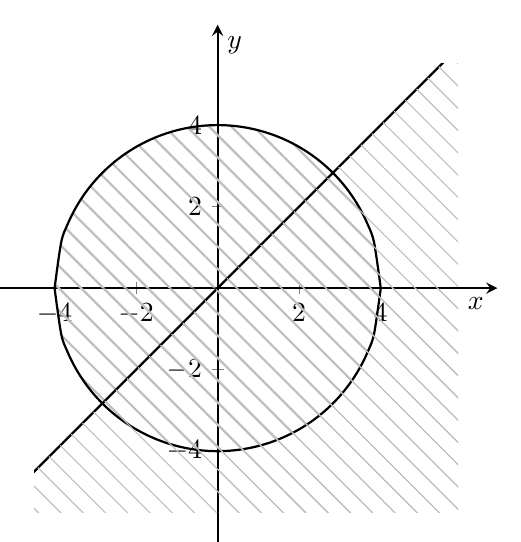
\begin{tikzpicture}
\begin{axis}[ 
xlabel=$x$,
ylabel=$y$,
axis x line=center, xlabel style={anchor=north west},
axis y line=center, ylabel style={anchor=south west},
xmin=-4.5,
xmax=5.9,
ymin=-5.5,
ymax=5.5,
axis line style={thick, shorten > = -0.5cm, shorten < = -0.5cm},
samples=50,
unit vector ratio*=1 1,
]
\addplot [domain=-4:4, thick, black, smooth,pattern={Lines[
                  distance=2mm,
                  angle=-45
                 ]},
        pattern color=gray!50]{sqrt(16-x^2)};
\addplot [domain=-4:4, thick, black, smooth,pattern={Lines[
                  distance=2mm,
                  angle=-45
                 ]},
        pattern color=gray!50]{-sqrt(16-x^2)};
\addplot [domain=-6:6, thick, black]{x};


\coordinate (A) at (axis cs:0,0) {};
\coordinate (B) at (axis cs:6,0) {};
\coordinate (C) at (axis cs:6,-6) {};
\coordinate (D) at (axis cs:0,-6) {};
\path[ pattern={Lines[
                  distance=2mm,
                  angle=-45
                 ]},
        pattern color=gray!50](A)--(B)--(C)--(D);

\coordinate (Ab) at (axis cs:-6,-6) {};
\coordinate (Bb) at (axis cs:6,6) {};
\coordinate (Cb) at (axis cs:6,-6) {};
\coordinate (Db) at (axis cs:-6,-6) {};

\path[ pattern={Lines[
                  distance=2mm,
                  angle=-45
                 ]},
        pattern color=gray!50](Ab)--(Bb)--(Cb)--(Db);

\begin{scope}

\coordinate (St) at (axis cs:4,-4.5) {};
%\draw [fill= white] (St) circle [radius=10.05];
%\node[right] at (St) {$B$};



\coordinate (Std) at (axis cs:-3,-4.5) {};
%\draw [fill= white] (Std) circle [radius=10.05];
%\node[above] at (Std) {$C$};


\coordinate (T) at (axis cs:-2,2.3) {};
%\draw [fill= white] (T) circle [radius=10.05];
%\node[below] at (T) {$A$};


\end{scope}
\end{axis};
\end{tikzpicture}
\caption{$\bigcup \mathscr{K}$}
\label{fig:fig_p8b}
\end{figure}
$$\lozenge$$
\textbf{c)} $\bigcup \mathscr{K}-\bigcap \mathscr{K}$
\begin{figure}[H]%
    \centering
   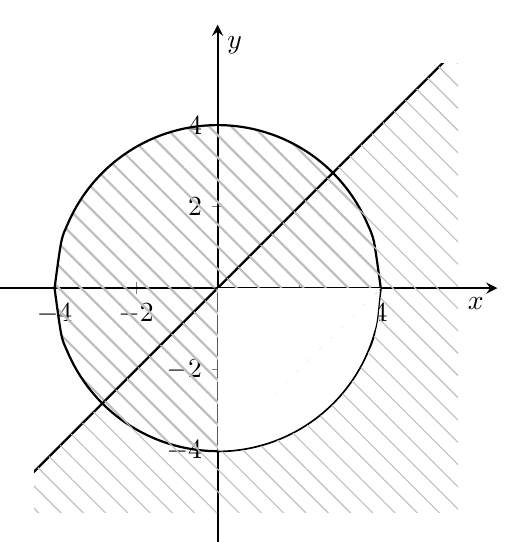
\begin{tikzpicture}
\begin{axis}[ 
xlabel=$x$,
ylabel=$y$,
axis x line=center, xlabel style={anchor=north west},
axis y line=center, ylabel style={anchor=south west},
xmin=-4.5,
xmax=5.9,
ymin=-5.5,
ymax=5.5,
axis line style={thick, shorten > = -0.5cm, shorten < = -0.5cm},
samples=50,
unit vector ratio*=1 1,
]
\addplot [domain=-4:4, thick, black, smooth,pattern={Lines[
                  distance=2mm,
                  angle=-45
                 ]},
        pattern color=gray!50]{sqrt(16-x^2)};
\addplot [domain=-4:4, thick, black, smooth,pattern={Lines[
                  distance=2mm,
                  angle=-45
                 ]},
        pattern color=gray!50]{-sqrt(16-x^2)};
\addplot [domain=-6:6, thick, black]{x};

\coordinate (Ab) at (axis cs:-6,-6) {};
\coordinate (Bb) at (axis cs:6,6) {};
\coordinate (Cb) at (axis cs:6,-6) {};
\coordinate (Db) at (axis cs:-6,-6) {};

\path[ pattern={Lines[
                  distance=2mm,
                  angle=-45
                 ]},
        pattern color=gray!50](Ab)--(Bb)--(Cb)--(Db);


\coordinate (A) at (axis cs:0,0) {};
\coordinate (B) at (axis cs:4,0) {};
\coordinate (C) at (axis cs:0,-4) {};
\coordinate (D) at (axis cs:0,-6) {};
\path[fill=white](A)--(B)--(C);

\begin{scope}

\coordinate (St) at (axis cs:4,-4.5) {};
%\draw [fill= white] (St) circle [radius=10.05];
%\node[right] at (St) {$B$};



\coordinate (Std) at (axis cs:-3,-4.5) {};
%\draw [fill= white] (Std) circle [radius=10.05];
%\node[above] at (Std) {$C$};


\coordinate (T) at (axis cs:-2,2.3) {};
%\draw [fill= white] (T) circle [radius=10.05];
%\node[below] at (T) {$A$};


\end{scope}
\addplot [domain=0:4,  black, smooth,fill=white]{-sqrt(16-x^2)};
\end{axis};
\end{tikzpicture}
\caption{$\bigcup \mathscr{K}-\bigcap \mathscr{K}$}
\label{fig:fig_p8b}
\end{figure}
$$\blacklozenge$$
\newpage
\subsection{}
\begin{tcolorbox}
Recall that $\mathbb{P}$ is the symbol for the set of positive integers. Suppose that for each $n\in \mathbb{P}$, we let $A_n=\{x\in \mathbb{R}: x\ge n\}$. Describe the sets $\bigcup\{A_n:n\in\mathbb{P}\}$ and $\bigcap\{A_n:n\in\mathbb{P}\}$.
\end{tcolorbox}

\textbf{$S=\bigcup\{A_n:n\in\mathbb{P}\}$} \\
$$S=[1,+\infty)$$
$$\lozenge$$
\textbf{   $\quad S=\bigcap\{A_n:n\in\mathbb{P}\}$} \\
$$S=\emptyset$$
This can be understood by the fact that for every $x\in\mathbb{R}$, you can find a $n\in\mathbb{P}$ so that $x\not\in A_n$. So, no $x$ can be an element of $S$.
$$\blacklozenge$$

\subsection{}
\begin{tcolorbox}
Suppose that for each $n\in \mathbb{P}$, $K_n$ is a non-empty set such that $K_{n+1}\subset K_n$. Let $\mathscr{K}=\{K_n:n\in \mathbb{P}\}$.\\
In each of the following, if the statement is necessarily true, say so and justify your answer. If the statement is not necessarily true, give a counterexample to justify your answer.
 \begin{align*}
\begin{array}{ll}
(a)&\bigcup \mathscr{K}=K_1\\
(b)&\bigcap \{K_i:i=1,2,\dots,n\}= K_n\\
(c)&\bigcap \mathscr{K}\ne \emptyset\\
\end{array}
\end{align*}
\end{tcolorbox}
(a) $\bigcup \mathscr{K}=K_1$.\\
\textbf{TRUE.\\}
Be $x\in K_n$ for any arbitrary $n$. So, $x\in K_n \cup K_{n-1}$. But $ K_n \cup K_{n-1} = K_{n-1}$, giving $x\in K_{n-1}$. Repeating that process with $K_{n-1}\subset K_{n-2}\subset \dots K_2\subset K_1$ we get $x\in K_n$.
$$\lozenge$$
(b) $\bigcap \{K_i:i=1,2,\dots,n\}= K_n$.\\
\textbf{TRUE.\\}
Suppose first that for all $n$ we have $K_n$ is a \textit{proper} subset of $K_{n-1}$. Then $ K_{n}\cap K_{n-1}=K_n$. Be $x\in K_n$ but not in $K_{n-1}$ for any arbitrary $n$. Then,  $x\in K_{n}\cap K_{n-1}$ is equivalent to $x\in K_n$. Repeating that process with we have $K_n\cap K_{n-1}\cap K_{n-2}\cap \dots K_2\cap K_1= K_n$ and get $x\in K_n$. Hence, $\bigcup \mathscr{K}=K_1$.\\
In the case that for some or all $n$ we have $K_n=K_{n-1}$ we could also state that  $\bigcap \{K_i:i=1,2,\dots,n\}= K_{n-1}$ but as $K_n=K_{n-1}$ we can write  $\bigcap \{K_i:i=1,2,\dots,n\}= K_{n-1}=K_n$.\\
The same is true in the case that a sequence of the subsets are proper subset of each other i.e. $K_{n+p}=K_{n+p-1}=\dots K_{n+1}=K_{n} = K_{n-1}=\dots =  K_{n-t}$. then one could write $\bigcap \{K_i:i=1,2,\dots,n\}= K_{n+p}$ but as $K_{n+p}=K_n$, the original statement holds.
$$\lozenge$$
(c) $\bigcap \mathscr{K}\ne \emptyset$.\\
\textbf{TRUE.\\}
As no $K_n$ is an empty set, $K_n$ will always contain at least one element and due to $(b)$ we get indeed $\bigcap \mathscr{K}\ne \emptyset$: suppose that for a given $n$, $K_n$ contains only one element $x$, then all subsequent $K_{n+p}$ must also have only one element i.e. $x$ and we will get $\bigcap \mathscr{K}=\{x\}$ 
$$\blacklozenge$$

\subsection{}
\begin{tcolorbox}
For each real number $r>0$, let $L_r=\{x:x\ge r\}$. Sketch the set $\bigcup \{L_r:r>0\}$ and $\bigcap\{L_r:r>0\}$ on a number line. If a set happens to be empty, say so.
\end{tcolorbox}
\begin{figure}[H]%
    \centering
    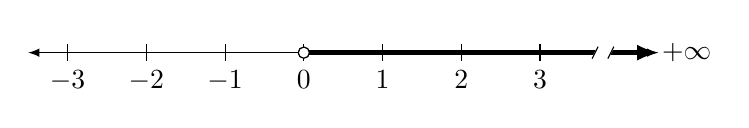
\begin{tikzpicture}
\draw[ultra thick,-latex] (0,0) -- (4.5,0);
\path [draw=black, fill=white] (0,0) circle (2pt);
%\path [draw=black, fill=black, thick] (4,0.0) circle (2pt);
\draw[latex-latex] (-3.5,0) -- (4.5,0) ;
\foreach \x in  {-3,-2,-1,0,1,2,3}
\draw[shift={(\x,0)},color=black] (0pt,3pt) -- (0pt,-3pt);
\foreach \x in {-3,-2,-1,0,1,2,3}
\draw[shift={(\x,0)},color=black] (0pt,0pt) -- (0pt,-3pt) node[below] 
{$\x$};
\draw[white,fill = white] (3.8,0.2) node (v1) {} -- (3.6,-0.2) node (v2) {} -- (3.8,-0.2) node (v4) {} -- (4,0.2) node (v3) {} -- (v1) -- cycle;
\draw  (v1) -- (v2);
\draw  (v3) -- (v4);
\node[anchor =  east] at (5.3,0){$+\infty$};
\path [draw=black, fill=white] (0,0) circle (2pt);
\end{tikzpicture}
\caption{$\bigcup \{L_r:r>0\}$}
\label{fig:fig_p8b}
\end{figure}
$$\lozenge$$
$\bigcap\{L_r:r>0\}=\emptyset$.\\

Indeed, take an arbitrary $r$ and  be $\epsilon > 0$ then $\exists x\in L_r: x\not \in L_{r+\epsilon}$. Then, $L_r\cap L_{r+\epsilon} =\emptyset$. So, whatever $L_r$ we choose in the collection $\mathscr{L}=\{L_r: r\in\mathbb{R}^+\}$ there always be a $L_{r^{'}}$ for which $L_r\cap L_{r^{'}}=\emptyset$ and hence $\bigcap\{L_r:r>0\}=\emptyset$.
$$\blacklozenge$$
\newpage

\subsection{}
\begin{tcolorbox}
Let $U$ be a set and let $\mathscr{K}$ be a non-empty collection of subsets of $U$. $\sim$ will signify the complement with respect to $U$. Prove the following set identities. The identities are quite important and are known as De Morgan's Laws.
\begin{align*}
\begin{array}{ll}
(a)&\sim(\bigcup \{K:K\in \mathscr{K}\}) = \bigcap\{\sim K:K\in \mathscr{K}\}\\
(b)&\sim(\bigcap \{K:K\in \mathscr{K}\}) = \bigcup\{\sim K:K\in \mathscr{K}\}\\
\end{array}
\end{align*} 
\end{tcolorbox}
(a) $\sim(\bigcup \{K:K\in \mathscr{K}\}) = \bigcap\{\sim K:K\in \mathscr{K}\}$\\
Suppose $x\in\,  \sim(\bigcup \{K:K\in \mathscr{K}\})$, then $x\not\in \bigcup \{K:K\in \mathscr{K}\}$. This means that $x$ is not an element of any $K\in \mathscr{K}$ i.e. $\forall K\in \mathscr{K}: x\not\in K$. This can also be expressed as  $\forall K\in \mathscr{K}: x\in\, \sim K)$. This means that $x$ is an element of all $\sim K$ giving $x\in \bigcap\{\sim K:K\in \mathscr{K}\}$ and thus $\sim(\bigcup \{K:K\in \mathscr{K}\}) \subset \bigcap\{\sim K:K\in \mathscr{K}\}$.\\
Suppose now that $x\in \bigcap\{\sim K:K\in \mathscr{K}\}$. This means that $x$ is an element of  $\{\sim K: K\in \mathscr{K}\}$ for all $K$ i.e. $x\not \in \{K: K\in \mathscr{K}\}$ for all $K$, (indeed if $x$ would be an element of a $K\in  \mathscr{K}$ then $x$ would not be an element of its complement and so $x$ could not be an element of $\bigcap\{\sim K:K\in \mathscr{K}\}$). The conclusion is that $x\not\in \bigcup \{K:K\in \mathscr{K}\}$ and thus $x\in \sim\bigcup \{K:K\in \mathscr{K}\}$. Hence, $\bigcap\{\sim K:K\in \mathscr{K}\}\subset \sim(\bigcup \{K:K\in \mathscr{K}\})$. \\
Conclusion $\sim(\bigcup \{K:K\in \mathscr{K}\}) = \bigcap\{\sim K:K\in \mathscr{K}\}$.
$$\lozenge$$
(b) $\sim(\bigcap \{K:K\in \mathscr{K}\}) = \bigcup\{\sim K:K\in \mathscr{K}\}$\\
Suppose $x\in\,  \sim(\bigcap \{K:K\in \mathscr{K}\})$, then $x\not\in \bigcap \{K:K\in \mathscr{K}\}$. This means that there exists at least one $K\in \mathscr{K}$ so that $x$ is not an element of this  $K$ i.e. $\exists K\in \mathscr{K}: x\not\in K$. This can also be expressed as  $\exists K\in \mathscr{K}: x\in\, \sim K$. This means that $x$ is an element of  $\bigcup\{\sim K:K\in \mathscr{K}\}$ and thus $\sim(\bigcap \{K:K\in \mathscr{K}\}) \subset \bigcup\{\sim K:K\in \mathscr{K}\}$. \\
Suppose now that $x\in \bigcup\{\sim K:K\in \mathscr{K}\}$. This means that $x$ is an element of  at least one $\sim K: K\in   \mathscr{K}$. Stated differently, there exist at least one $ K: K\in   \mathscr{K}$ for which $x\not \in K$. This means that $x$ can not be an element of $\bigcap \{K:K\in \mathscr{K}\}$ and thus $x\in \, \sim \bigcap \{K:K\in \mathscr{K}\}$ which means $\bigcup\{\sim K:K\in \mathscr{K}\}\subset \, \sim(\bigcup \{K:K\in \mathscr{K}\})$\\
Conclusion $\sim(\bigcap \{K:K\in \mathscr{K}\}) = \bigcup\{\sim K:K\in \mathscr{K}\}$.
$$\blacklozenge$$
\newpage
\subsection{}
\begin{tcolorbox}
Let $S=\{1,2,3,4,5\}$ and let $\mathscr{P}(S)$ be the power set of $S$. List the elements in $\mathscr{P}(S)$.
\end{tcolorbox}
We order them according to the number of elements in the subsets. We check the number of subsets by using the $\binom{5}{m}$ formula (i.e. combination without repetition). 
\begin{align*}
5 \text{ elements}\quad \binom{5}{5}= 1\\
\{1,2,3,4,5\}\\
4 \text{ elements}\quad \binom{5}{4}= 5\\
\{1,2,3,4\}\\
\{1,2,3,5\}\\
\{1,2,4,5\}\\
\{1,3,4,5\}\\
\{2,3,4,5\}\\
3 \text{ elements}\quad \binom{5}{3}= 10\\
\{1,2,3\}\\
\{1,2,4\}\\
\{1,2,5\}\\
\{1,3,4\}\\
\{1,3,5\}\\
\{1,4,5\}\\
\{2,3,4\}\\
\{2,3,5\}\\
\{2,4,5\}\\
\{3,4,5\}\\
\end{align*}
\begin{align*}
2 \text{ elements}\quad \binom{5}{2}= 10\\
\{1,2\}\\
\{1,3\}\\
\{1,4\}\\
\{1,5\}\\
\{2,3\}\\
\{2,4\}\\
\{2,5\}\\
\{3,4\}\\
\{3,5\}\\
\{4,5\}\\
\end{align*}
\begin{align*}
1\text{ element}\quad \binom{5}{1}= 5\\
\{1\}\\
\{2\}\\
\{3\}\\
\{4\}\\
\{5\}\\
0\text{ elements}\quad \binom{5}{0}= 1\\
\emptyset\\
\end{align*}
Note that the total number of subsets in $\mathscr{P}(S)$ is $1+5+10+10+5+1 = 32$ which corresponds to $2^5$.
$$\blacklozenge$$
\newpage

 \section{Cartesian Product}
\subsection{}
\begin{tcolorbox}
Suppose that $A\subset B$ and $C$ is a set. Prove that $A\times C\subset B\times C$.
\end{tcolorbox}
Be $x\in A$ and $y\in C$. As $A\subset B$, then $x$ is also in $B$. Thus $\underbrace{(x,y)}_{x\in A,\, y\in C}\in A\times C$ means also that $\underbrace{(x,y)}_{x\in B,\, y\in C}\in B\times C$
$$\blacklozenge$$

\subsection{}
\begin{tcolorbox}
Let $A=\{1,2,3\}$, $B=\{a,b\}$, and $C=\{\alpha,\beta\}$. List the elements of each of the following sets:
\begin{align*}
\begin{array}{ll}
(a)&A\times (B\cup C)\\
(b)&(A\times B)\cup(A\times C)\\
(c)&(A\cup B)\times C\\
(d)&(A\times C)\cup(B\times C)\\
\end{array}
\end{align*} 
\end{tcolorbox}
(a) $A\times (B\cup C)$\\\\
$(1,a),\,(1,b),\,(2,a),\,(2,b),\,(3,a),\,(3,b)$\\ 
$(1,\alpha),\,(1,\beta),\,(2,\alpha),\,(2,\beta),\,(3,\alpha),\,(3,\beta)$ 
$$\lozenge$$

(b) $(A\times B)\cup(A\times C)$\\\\
$(1,a),\,(1,b),\,(2,a),\,(2,b),\,(3,a),\,(3,b)$\\ 
$(1,\alpha),\,(1,\beta),\,(2,\alpha),\,(2,\beta),\,(3,\alpha),\,(3,\beta)$ 
$$\lozenge$$

(c) $(A\cup B)\times C$\\\\
$(1,\alpha),\,(1,\beta),\,(2,\alpha),\,(2,\beta),\,(3,\alpha),\,(3,\beta)$ 
$(1,\alpha),\,(1,\beta),\,(2,\alpha),\,(2,\beta),\,(3,\alpha),\,(3,\beta)$ \\
$(a,\alpha),\,(a,\beta),\,(b,\alpha),\,(b,\beta)$ 
$$\lozenge$$

(d) $(A\times C)\cup(B\times C)$\\\\
$(1,\alpha),\,(1,\beta),\,(2,\alpha),\,(2,\beta),\,(3,\alpha),\,(3,\beta)$ 
$(1,\alpha),\,(1,\beta),\,(2,\alpha),\,(2,\beta),\,(3,\alpha),\,(3,\beta)$ \\
$(a,\alpha),\,(a,\beta),\,(b,\alpha),\,(b,\beta)$ 
$$\blacklozenge$$
\newpage
\subsection{}
\begin{tcolorbox}
Are any of the sets in Exercise 2 the same? If so write the set identities that are suggested by your observations. Try to prove your conjecture.
\end{tcolorbox}
In exercise 2 we can see that that the set (a) and (b) are the same. Also (c) and (d) are the same. This suggests the following identities $A\times (B\cup C)=(A\times B)\cup(A\times C)$ and $(A\cup B)\times C=(A\times C)\cup(B\times C)$. \\\\
$\mathbf{A\times (B\cup C)=(A\times B)\cup(A\times C)}$\\
Proof:\\
Be $x\in A$ and $ y\in B\cup C$, so $y$ is an element of $B$ or $C$. Consider $(x,y)\in A\times (B\cup C)$. As the $y$ can be an element of $B$ or $C$  follows immediately that $(x,y)\in (A\times B)$ or $(x,y)\in A\times C)$ and thus  $(x,y)\in (A\times B)\cup(A\times C)$. And get $A\times (B\cup C)\subset(A\times B)\cup(A\times C)$ \\
Suppose now that $(x,y)\in (A\times B)\cup(A\times C)$. The $(x,y)$ is an element of $A\times B$ or $A\times C$. For the same $x\in A$ this implies that $y\in B$ or $y\in C$ and thus $(x,y) \in A\times (B\cup C)$, giving $(A\times B)\cup(A\times C)\subset A\times (B\cup C)$ leading with the previous  $A\times (B\cup C)=(A\times B)\cup(A\times C)$.
$$\lozenge$$
$\mathbf{(A\cup B)\times C=(A\times C)\cup(B\times C)}$\\
Proof:\\
Be $x\in A\cup B $ and $ y\in  C$, so $x$ is an element of $A$ or $B$. Consider $(x,y)\in(A\cup B)\times C$. As the $x$ can be an element of $A$ or $B$  follows immediately that $(x,y)\in (A\times C)$ or $(x,y)\in (B\times C)$ and thus  $(x,y)\in (A\times B)\cup(\textbf{A}\times C)$. And get $(A\cup B)\times C\subset(A\times C)\cup(B\times C)$ \\
Suppose now that $(x,y)\in (A\times B)\cup(\textbf{A}\times C)$. The $(x,y)$ is an element of $A\times C$ or $B\times C$. For the same $y\in C$ this implies that $x\in A$ or $x\in B$ and thus $(x,y) \in (A\times C)\cup(B\times C)$, giving $(A\times C)\cup(B\times C)\subset (A\cup B)\times C$ leading with the previous  $(A\cup B)\times C=(A\times C)\cup(B\times C)$.
$$\blacklozenge$$

\subsection{}
\begin{tcolorbox}
Suppose that $A$ is a set consisting of five elements and $B$ is a set consisting of three elements. How many elements does the set $A\times B$ have? The set $B\times A$?
\end{tcolorbox}
$A\times B$ has $5\times 3 =15$ elements. Indeed in the element $(x,y) \in A\times B$  we can choose for $x$ out of the five elements of $A$ and for each choice of $x$ we are free to choose one element out of the $3$ elements of $B$.\\
For $B\times A$, the reasoning is the same and get $3\times 5=15$ elements.
$$\blacklozenge$$

\subsection{}
\begin{tcolorbox}
Suppose that $A$ is a set consisting of $m$ elements and $B$ is a set consisting of $n$ elements, where $m$ and $n$ are positive integers. How many elements are there in  $A\times B$?
\end{tcolorbox}
$A\times B$ has $m\times m $ elements. Indeed in the element $(x,y) \in A\times B$  we can choose for $x$ out of the $m$ elements of $A$ and for each choice of $x$ we are free to choose one element out of the $n$ elements of $B$.
$$\blacklozenge$$

\subsection{}
\begin{tcolorbox}
Suppose that $A$ is a set consisting of three elements, $B$ consists of four elements and $C$ consists of two element. How many elements are there in the set   $(A\times B)\times$?
\end{tcolorbox}
$(A\times B)\times C$ has $(3\times 4)\times 2 = 24 $ elements. Indeed in the element $\left((x,y), z\right) \in (A\times B)\times C $  we have  for $(x,y)$,  $3\times 4 =12$ elements (see Exercise $1.9.5$) and for each choice of this $(x,y)$ we are free to choose one element out of the $2$ elements of $C$.
$$\blacklozenge$$\newpage

 \section{Functions}
\subsection{}
\begin{tcolorbox}
In each of the following, a set of ordered pairs $\Gamma$ is given. In each case, determine whether $\Gamma$ is a function and, if it is, determine if it is a one-to-one function.
\begin{align*}
\begin{array}{ll}
(a)&\text{Let } \Gamma=\{(x,y):-1\le x\le 1 \text{ and } x^2+y^2=1\}.  \\
(b)&\text{Let } \Gamma=\{(x,y):-1\le x\le 1,\, y \ge 0, \text{ and } x^2+y^2=1\}.  \\
(c)&\text{Let } \Gamma=\{(x,y):0\le x\le 1 \text{ and } x^2+y^2=1\}.  \\
(d)&\text{Let } \mathscr{F}\text{ be the collection of all real-valued differentiable functions }\\ 
&\text{ defined on the open interval } (a,b). \\
&\text{Let }\Gamma=\{(f,f^{'}):f\in\mathscr{F} \text{ and }f^{'} \text{ is the derivative of } f\}.  \\
(e)&\text{Let } X \text{ be the collection of all continuous real-valued functions }\\ 
&\text{ defined on the closed interval } [a,b]. \\
&\text{Let }\Gamma=\left\{\left ( f,\int_a^b f(x)dx\right):f\in X  \right \}.  \\
\end{array}
\end{align*} 
\end{tcolorbox}
(a) $\text{Let } \Gamma=\{(x,y):-1\le x\le 1 \text{ and } x^2+y^2=21\}$\\\\
$\Gamma$ is not a function due to the ambiguity of the $\sqrt{\quad}$ function. E.g. take $x=0$ then $y =\pm1$.
$$\lozenge$$

(b) $\text{Let } \Gamma=\{(x,y):-1\le x\le 1,\, y \ge 0, \text{ and } x^2+y^2=1\}. $ \\\\
This time, as the ambiguity on the range has been removed by the condition $y\ge0$ $\Gamma$ is a function. Yet, it is not one-to-one e.g. for $x=-1$ and $x=1$ we get the same value for $y$.
$$\lozenge$$

(c) $\text{Let } \Gamma=\{(x,y):0\le x\le 1 \text{ and } x^2+y^2=2\}. $ \\\\
This time, as the ambiguity on the range has been removed by the condition $y\ge0$ $\Gamma$ is a function. And,  it is a one-to-one function as with the restriction on the domain $x\in [0,1]$ , $y$ is well and uniquely defined.
$$\lozenge$$

(d) $\text{Let } \mathscr{F}\text{ be the collection of all real-valued differentiable functions }\\ 
\text{ defined on the open interval } (a,b). 
\text{Let }\Gamma=\{(f,f^{'}):f\in\mathscr{F} \text{ and }f^{'} \text{ is the derivative of } f\}.$ \\\\
$\Gamma$ is a function as $f$ is a real-valued differentiable function, meaning that $\forall f\in \mathscr{F}, \exists f^{'}$.\\
Yet, it is not one-to-one. E.g. take $f_1 = x+1$ and $f_2= x+2$, both function give $f^{'}= 1$ meaning that $\Gamma$ is not one-to-one.
$$\lozenge$$
(e) $\text{Let } X \text{ be the collection of all continuous real-valued functions }\\ 
\text{ defined on the closed interval } [a,b]. \\
\text{Let }\Gamma=\left\{\left ( f,\int_a^b f(x)dx\right):f\in X  \right \}.  $ \\\\
$\Gamma$ is a function as $f$ is a continuous real-valued function, and from calculus we know that every continuous is Riemann-integrable, meaning that for every $f$ there exist a real number $\int_a^b f(x)dx$. Yet,  $\Gamma$ is not one-to-one as two  
different functions $f_1$ and $f_2$ could have the same value of their integral on the given domain e.g. take $f_1= \frac{x-a}{b-a}$ and $f_2= \frac{b-x}{b-a}$, both have the same value for the integral over $[a,b]$ namely $\half(b-a)$.
$$\blacklozenge$$

\subsection{}
\begin{tcolorbox}
Let $f:\mathbb{R}\times \mathbb{R}\rightarrow \mathbb{R}\times \mathbb{R}$ be the function defined as follows: \\
For each $(x,y) \in \mathbb{R}$, let $f(x,y) = (a,b)$ where
$$a= x+ 2y$$
and
$$b= 2x+4y$$
Which of the following terms applies to  $f:\mathbb{R}\times \mathbb{R}\rightarrow \mathbb{R}\times \mathbb{R}$ ?\\
(a) surjective, (b) bijective, (c) injective.
\end{tcolorbox}
$f$ in not injective. Indeed the given function definition can be considered as a system of linear equations with $x$ and $y$ as unknowns and $a,\, b$ as parameters. So for a given $(a,b)  \in \mathbb{R}\times \mathbb{R}$ (the domain) the range will only span $\mathbb{R}\times \mathbb{R}$ only if the system of equations is not degenerated i.e. if the determinant of the system is not $0$, but we have $$det\left(\begin{matrix}1&2\\2&4\end{matrix}\right) =0$$
Hence, $f$ is not surjective. It is however one-to-one (injective) as for a given $(x,\, y)$, due to linear form of the function, there will be only one $(a,\, b)$ on which $(x,\, y)$ is mapped. As $f$ is not surjective, $f$ can not be bijective.
$$\blacklozenge$$
\newpage
\subsection{}
\begin{tcolorbox}
Repeat the question in Ecercise $2$ for the system
$$a= 3x+ 2y$$
$$b= 6x-2y$$
\end{tcolorbox}
$f$ is injective as we see that this time the determinant of the system is  $$det\left(\begin{matrix}3&2\\6&-2\end{matrix}\right) =-18$$
Hence, $f$ is surjective. It is also one-to-one (injective) for the same reason mentioned in Exercise 2. . As $f$ is  surjective and injective , $f$ is also bijective.
$$\blacklozenge$$

\subsection{}
\begin{tcolorbox}
Let $f$ be a map from the set of all reals $\mathbb{R}$ into $\mathbb{R}$. Suppose furthermore that if $x_1$ and $x_2$ are in $\mathbb{R}$ and $x_1 < x_2$, then  $f(x_1) < f(x_2)$. Is it necessarily true that $f$ is one-to-one? Is it necessarily true that $f[\mathbb{R}]= \mathbb{R}$? Justify your answer.
\end{tcolorbox}
It is necessarily true that $f$ is one-to-one. (At each point $x_1$, the function for a given $x_2$ could be re-written as $f(x_2)= f(x_1) + \phi(x_1)(x_2-x_1)$ with $\phi(x_1)>0$. So $f(x_2)$ can not be equal to $f(x_1)$ unless $x_2=x_1$.)\\
On the other hand $f[\mathbb{R}]$ is not necessarily equal to $ \mathbb{R}$. As a counterexample, consider the function $f(x)= e^{-x}$, which is a monotone increasing function but the range is $(-\infty,0)\ne \mathbb{R}$
$$\blacklozenge$$

\subsection{}
\begin{tcolorbox}
Consider the function $f:X\rightarrow Y$. Suppose that $A$ and $B$ are subsets of $X$. Decide which of the following statements are necessarily true. Justify your answers.
\begin{align*}
\begin{array}{ll}
(a)&\text{If } A\cap B =\emptyset, \text{ then } f[A]\cap f[B]=\emptyset . \\
(b)&\text{If } f[A]\cap f[B]=\emptyset, \text{ then }  A\cap B =\emptyset .  \\
(c)& \text{If } A\subset B , \text{ then } f[A]\subset f[B].  \\
(d)&f[A-B] = f[A]-f[B].  \\
(e)&f[A\cup B]= f[A]\cup f[B].  \\
(f)&f[A\cap B]\subset f[A]\cap f[B].  \\
(g)&f[A\cap B]= f[A]\cap f[B].  \\
\end{array}
\end{align*}
\end{tcolorbox}
(a) If $A\cap B =\emptyset, \text{ then } f[A]\cap f[B]=\emptyset $. \\
This is not necessarily true. Take for example a non injective function like $f(x)=\sin(x)$  then $f[[0,\frac{\pi}{4}]]\cap f[\frac{3\pi}{4}, \pi]= [0,\frac{\sqrt{2}}{2}]$. 
$$\lozenge$$

(b) If $f[A]\cap f[B]=\emptyset, \text{ then }  A\cap B =\emptyset$ \\
This is  necessarily true as for $f$ being a function we have $\left( x_2,f(x_2)\right)\in f$ and $\left( x_1,f(x_1)\right)\in f \Rightarrow f(x_1)=f(x_2)$ and $ A\cap B \ne\emptyset$ would mean that $\exists x\in A\cap B$ for which $x$ has two different images.
$$\lozenge$$

(c) If $A\subset B , \text{ then } f[A]\subset f[B].$ \\
This is  necessarily true as for the same reason as in $(b)$.
$$\lozenge$$

(d)  $f[A-B] = f[A]-f[B]$ \\
This is  not necessarily true. Let's take the same counterexample as in $(a)$ i.e. $f(x)=\sin(x)$  and let's define $A= [0,2\pi]$, $B=[0,\frac{\pi}{4}]$, then $f[A] =  [-1,1]$ and $f[B]=[0,\frac{\sqrt{2}}{2}]$ and $f[A]-f[B] =  [-1,0)\cup (\frac{\sqrt{2}}{2},1]$ while $f[A-B]=[-1,1]$.
$$\lozenge$$

(e)  $f[A\cup B]= f[A]\cup f[B]$ \\
This is  true. \\
Suppose first that $A\cap B=\emptyset$ and take $x\in A$, then $f(x) \in f[A]$ and $x\not \in f[B]$ giving $f(x)\in f[A]\cup f[B]$. On the other hand it is obvious that if $A\cap B\ne\emptyset$ then $f(x) \in f[A]$ and-or $f(x) in f[B]$ giving $f(x) \in f[A]\cup f[B]$. Hence, $f[A\cup B]\subset f[A]\cup f[B]$.\\
Suppose now that $f(x) \in f[A]$ this means that $x\in A$ regardless of $x\in B$ or not. So, $f[A]\cup f[B]\subset f[A\cup B]$ and with the previous we get $f[A\cup B]= f[A]\cup f[B]$.
$$\lozenge$$

(f)  $f[A\cap B]\subset f[A]\cap f[B]$ \\
True as if $f(x) \in f[A\cap B]$ means that $x\in A\cap B$ so $x $ will be mapped in the image $f[A]$ and in the image $f[B]$ and thus $f[A\cap B]\subset f[A]\cap f[B]$.
$$\lozenge$$

(g)  $f[A\cap B] = f[A]\cap f[B]$ \\
Not true.
Suppose $f(x) \in f[A]\cap f[B]$. But if $f$ is not injective the possibility exists that for a given $x_a\in A$ and another $x_b \in B$ we have $f[x_a]= f[x_b]$ even if $A$ and $B$ are disjoint sets which would give $f[A\cap B]=f[\emptyset]=\emptyset$.
$$\blacklozenge$$
\newpage


 \section{Relations}
 In Exercises $1$ to $5$, all relations are subsets of the plane. In each case, draw a sketch of $R$, and give $\text{Dom}R,\, \text{ Range} R,\, R[0] \text{ and  } R^{-1}[0]$.
\subsection{}
\begin{tcolorbox}
 Let $(x,y)\in R$ provided that $(x,y)$ satisfies each of the following inequalities: $x+y\le 3,\,y-x \ge 0,\, x \ge -3$.
\end{tcolorbox}
\begin{figure}[H]%
    \centering
    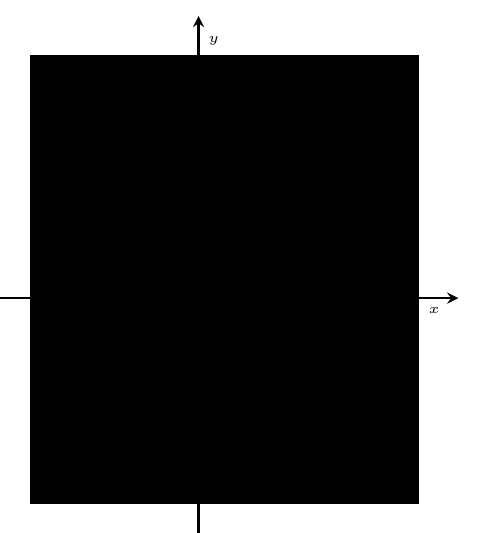
\begin{tikzpicture}
\begin{axis}[ 
xlabel=$x$,
ylabel=$y$,
axis x line=center, xlabel style={anchor=north west},
axis y line=center, ylabel style={anchor=south west},
xmin=-4.5,
xmax=5.9,
ymin=-5.5,
ymax=6.5,
axis line style={thick, shorten > = -0.5cm, shorten < = -0.5cm},
samples=50,
unit vector ratio*=1 1,
font=\tiny
]



\addplot [domain=-6:6, thick, black, smooth,fill=white]{3-x};
\addplot [domain=-6:6, thick, black, smooth,fill=white]{x};


\coordinate (A) at (axis cs:7,7) {};
\coordinate (B) at (axis cs:-6,-6) {};
\coordinate (C) at (axis cs:-6,7) {};
\coordinate (D) at (axis cs:6,7) {};
\path[ pattern={Lines[
                  distance=2mm,
                  angle=-45
                 ]},
        pattern color=gray!50](A)--(B)--(C);
        
 \coordinate (At) at (axis cs:6,-3) {};
\coordinate (Bt) at (axis cs:-6,9) {};
\coordinate (Ct) at (axis cs:-6,-6) {};
\coordinate (Dt) at (axis cs:6,-9) {};
\path[ pattern={Lines[
                  distance=2mm,
                  angle=45
                 ]},
        pattern color=gray!50](At)--(Bt)--(Ct)--(Dt);
        
        \path[ pattern={Lines[
                  distance=2mm,
                  angle=0
                 ]},
        pattern color=gray!50](axis cs:-3,-6)--(axis cs:-3,7)--(axis cs:6,7)--(axis cs:6,-6);
 \draw [](axis cs:-3,-6)--(axis cs:-3,7);       
\draw [](axis cs:-4,0)--(axis cs:4,0);
\draw [](axis cs:0,4)--(axis cs:0,-4);

\begin{scope}
\coordinate (S) at (axis cs:4,4) {};
\coordinate (St) at (axis cs:2.5,5.5) {};
\draw [fill= white] (S) circle [radius=10.05];
\node[above right] at (St) {$y-x\ge 0$};
\draw[-{Latex[length=2mm]}] (S) --(St);

\coordinate (Sd) at (axis cs:5,-2) {};
\coordinate (Std) at (axis cs:2.5,-4.5) {};
\draw [fill= white] (Sd) circle [radius=10.05];
\node[below] at (Std) {$y+x\le 3$};
\draw[-{Latex[length=2mm]}] (Sd) --(Std);

\coordinate (P) at (axis cs:-3,-4.5) {};
\coordinate (Pt) at (axis cs:-1,-4.5) {};
\draw [fill= white] (P) circle [radius=10.05];
\node[below right] at (P) {$x\ge-3$};
\draw[-{Latex[length=2mm]}] (P) --(Pt);


\coordinate (T) at (axis cs:2.7,2.3) {};
\coordinate (Tt) at (axis cs:-2.7,-3) {};
%\draw [fill= white] (T) circle [radius=1.05];
%\node[below] at (Tt) {$A$};
%\draw[-{Latex[length=2mm]}] (T) --(Tt);
\coordinate (P1) at (axis cs:-3,6) {};
\coordinate (P2) at (axis cs:1.5,1.5) {};
\coordinate (P2a) at (axis cs:1.5,0) {};
\coordinate (P3) at (axis cs:-3,-3) {};
\coordinate (P4) at (axis cs:0,3) {};
\coordinate (P5) at (axis cs:-3,0) {};
\coordinate (P0) at (axis cs:-0,0) {};
\draw [fill= black] (P1) circle [radius=10.05];
\draw [fill= black] (P2) circle [radius=10.05];
\draw [fill= black] (P2a) circle [radius=10.05];
\draw [fill= black] (P3) circle [radius=10.05];
\node[below left] at (P1) {$P_1$};
\node[right] at (P2) {$P_2$};
\node[above right] at (P2a) {$P_2^{'}$};
\node[above left] at (P3) {$P_3$};

\draw [fill= black] (P0) circle [radius=10.05];
\draw [fill= black] (P4) circle [radius=10.05];
\draw [fill= black] (P5) circle [radius=10.05];
\node[below right] at (P0) {$P_0$};
\node[right] at (P4) {$P_4$};
\node[above left] at (P5) {$P_5$};
\draw [dashed, thin] (P2)--(P2a);
\end{scope}

\end{axis};
\end{tikzpicture}
\caption{$x+y\le 3,\,y-x \ge 0,\, x \ge -3$}
\label{fig:fig_p8b}
\end{figure}
$$ $$
\textbf{$\text{Dom}R$} $=\text{segment }[P_5,P_2^{'}]$\\
\textbf{$\text{Range} R$} $=\text{segment }[P_3,P_1]$\\
\textbf{$R[0]$ }: $=\text{segment }[P_0,P_4]$\\
\textbf{$R^{-1}[0]$}: $=\text{segment }[P_5,P_0]$
$$\blacklozenge$$

\subsection{}
\begin{tcolorbox}
 Let $R$ be the set of all $(x,y)$ that satisfy $x^2-y^2\le 1$ and $y^2-x^2 \le 1$.
\end{tcolorbox}
\begin{figure}[H]%
    \centering
    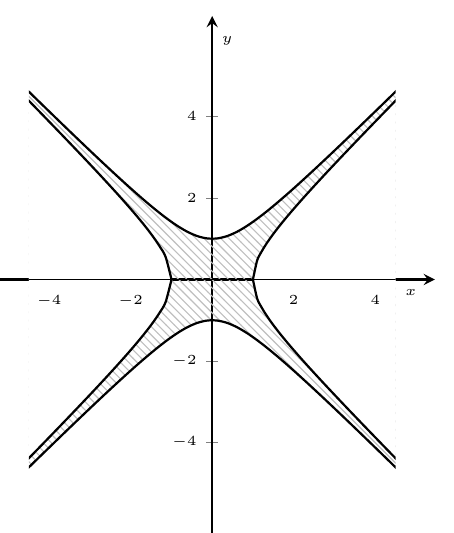
\begin{tikzpicture}
\begin{axis}[ 
xlabel=$x$,
ylabel=$y$,
axis x line=center, xlabel style={anchor=north west},
axis y line=center, ylabel style={anchor=south west},
xmin=-4.5,
xmax=4.5,
ymin=-5.5,
ymax=5.5,
axis line style={thick, shorten > = -0.5cm, shorten < = -0.5cm},
samples=50,
unit vector ratio*=1 1,
font=\tiny
]

\addplot [name path=A,domain=-6:1, thick, black, smooth]{sqrt(x^2-1)};
\addplot [name path=B,domain=-6:1, thick, black, smooth]{-sqrt(x^2-1)};

\addplot [name path=C,domain=1:6, thick, black, smooth]{sqrt(x^2-1)};
\addplot [name path=D,domain=1:6, thick, black, smooth]{-sqrt(x^2-1)};        
        

        
\addplot [name path=E,domain=-6:6, thick, black, smooth]{sqrt(1+x^2)};
\addplot [name path=F,domain=-6:6, thick, black, smooth]{-sqrt(1+x^2)};
        

\addplot[pattern=north west lines, pattern color=gray!50]fill between[of=E and F , soft clip={domain=-6:6}];
\addplot[ color=white]fill between[of=A and B , soft clip={domain=-6:6}];
\addplot[color=white]fill between[of=C and D , soft clip={domain=-6:6}];
\draw [](axis cs:-6,0)--(axis cs:6,0);
\end{axis};
\end{tikzpicture}
\caption{$x^2-y^2\le 1$ and $y^2-x^2 \le 1$}
\label{fig:fig_p8b}
\end{figure}
$$ $$
\textbf{$\text{Dom}R$} $=(-\infty,+\infty)$\\
\textbf{$\text{Range} R$} $=(-\infty,+\infty)$\\
\textbf{$R[0]$ }: $=[-1,1]$\\
\textbf{$R^{-1}[0]$}: $=[-1,1]$\\
$$\blacklozenge$$

\subsection{}
\begin{tcolorbox}
 Let $R$ be the set of all $(x,y)$ such that $x-y$ is a multiple of 3.
\end{tcolorbox}
\begin{figure}[H]%
    \centering
    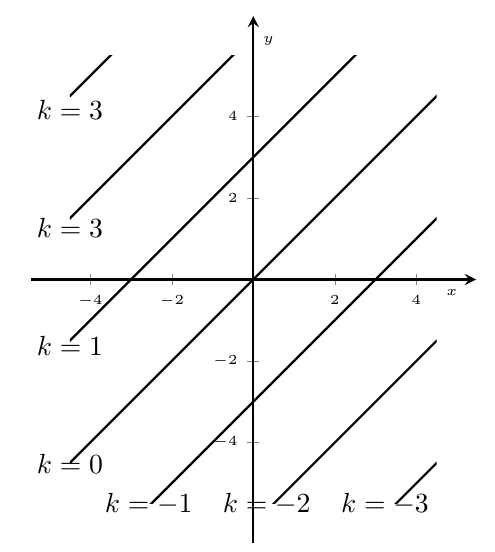
\begin{tikzpicture}
\begin{axis}[ 
xlabel=$x$,
ylabel=$y$,
axis x line=center, xlabel style={anchor=north west},
axis y line=center, ylabel style={anchor=south west},
xmin=-4.5,
xmax=4.5,
ymin=-5.5,
ymax=5.5,
axis line style={thick, shorten > = -0.5cm, shorten < = -0.5cm},
samples=50,
unit vector ratio*=1 1,
font=\tiny
]

\addplot [name path=A,domain=-6:6, thick, black, smooth]{x-3*4)};
\addplot [name path=A,domain=-6:6, thick, black, smooth]{x-3*3)};
\addplot [name path=A,domain=-6:6, thick, black, smooth]{x-3*2)};
\addplot [name path=A,domain=-6:6, thick, black, smooth]{x-3*1)};
\addplot [name path=A,domain=-6:6, thick, black, smooth]{x-3*0)};
\addplot [name path=A,domain=-6:6, thick, black, smooth]{x+3*4)};
\addplot [name path=A,domain=-6:6, thick, black, smooth]{x+3*3)};
\addplot [name path=A,domain=-6:6, thick, black, smooth]{x+3*2)};
\addplot [name path=A,domain=-6:6, thick, black, smooth]{x+3*1)};

\end{axis};
\node at (0,5) {$k=3$};
\node at (0,3.5)  {$k=3$};
\node at (0,2)  {$k=1$};;
\node at (0,0.5)  {$k=0$};
\node at (1,0)  {$k=-1$};;
\node at (2.5,0)  {$k=-2$};
\node at (4,0)  {$k=-3$};
\end{tikzpicture}
\caption{The relation $\{(x,y): y=x-3k, k\in \mathbb{Z}$}
\label{fig:fig_p8b}
\end{figure}
$$ $$
\textbf{$\text{Dom}R$} $=(-\infty,+\infty)$\\
\textbf{$\text{Range} R$} $=(-\infty,+\infty)$\\
\textbf{$R[0]$ }: $=\{y: y=3k, k\in\mathbb{Z}\}$\\
\textbf{$R^{-1}[0]$}: $=\{x: x=3k, k\in\mathbb{Z}\}$\\
$$\blacklozenge$$

\subsection{}
\begin{tcolorbox}
 Let $R$ be a subset of the plane such that $(x,y)\in R$ provided that $x-y\le \half$
\end{tcolorbox}
\begin{figure}[H]%
    \centering
    \begin{tikzpicture}
\begin{axis}[ 
xlabel=$x$,
ylabel=$y$,
axis x line=center, xlabel style={anchor=north west},
axis y line=center, ylabel style={anchor=south west},
xmin=-4.5,
xmax=5.9,
ymin=-5.5,
ymax=6.5,
axis line style={thick, shorten > = -0.5cm, shorten < = -0.5cm},
samples=50,
unit vector ratio*=1 1,
font=\tiny
]



\addplot [domain=-6:6, thick, black, smooth,fill=white]{x-0.5};



\coordinate (A) at (axis cs:-6,6) {};
\coordinate (B) at (axis cs:6,6) {};
\coordinate (C) at (axis cs:6,5.5) {};
\coordinate (D) at (axis cs:-6,-6.5) {};
\path[ pattern={Lines[
                  distance=2mm,
                  angle=-45
                 ]},
        pattern color=gray!50](A)--(B)--(C)--(D);
        


\begin{scope}
\coordinate (S) at (axis cs:4,3.5) {};
\coordinate (St) at (axis cs:2.5,5) {};
\draw [fill= white] (S) circle [radius=10.05];
\node[above right] at (St) {$x-y\le \frac{1}{2}$};
\draw[-{Latex[length=2mm]}] (S) --(St);

\end{scope}

\end{axis};
\end{tikzpicture}
\caption{The relation $x-y\le \half$}
\label{fig:fig_p8b}
\end{figure}
$$ $$
\textbf{$\text{Dom}R$} $=(-\infty,+\infty)$\\
\textbf{$\text{Range} R$} $=(-\infty,+\infty)$\\
\textbf{$R[0]$ }:  $=[-\half,\infty)$\\
\textbf{$R^{-1}[0]$}:  $=(-\infty,\half]$\\
$$\blacklozenge$$
\newpage

\subsection{}
\begin{tcolorbox}
 Let $R$ be a subset of the plane such that $(x,y)\in R$ provided that $y=x^4$
\end{tcolorbox}
\begin{figure}[H]%
    \centering
    \begin{tikzpicture}
\begin{axis}[ 
xlabel=$x$,
ylabel=$y$,
axis x line=center, xlabel style={anchor=north west},
axis y line=center, ylabel style={anchor=south west},
xmin=-4.5,
xmax=5.9,
ymin=-5.5,
ymax=6.5,
axis line style={thick, shorten > = -0.5cm, shorten < = -0.5cm},
samples=50,
unit vector ratio*=1 1,
font=\tiny
]
\addplot [domain=-3:3, thick, black, smooth]{x*x*x*x};
 \end{axis};
\end{tikzpicture}
\caption{The relation $y=x^4$}
\label{fig:fig_p8b}
\end{figure}
$$ $$
\textbf{$\text{Dom}R$} $=(-\infty,+\infty)$\\
\textbf{$\text{Range} R$} $=[0,+\infty)$\\
\textbf{$R[0]$ }:  $=\{0\}$\\
\textbf{$R^{-1}[0]$}:  $=\{0\}$\\
$$\blacklozenge$$


\subsection{}
\begin{tcolorbox}
 Let $R=\{(x,y):x\ge 0,\, x^2+y^2=26\}$. Find $R[0],\, R[5],\text{ and } R[I]\text{, where } I= \{r:0\le r\le 1\};\, R^{-1}[J]\text{ where } J=  \{r:-1\le r\le 1\}$.
\end{tcolorbox}
$$ $$
\textbf{$R[0]$ }:  $=\{-\sqrt{26},\,\sqrt{26} \}$\\
\textbf{$R[5]$ }:  $=\{-1,\,1 \}$\\
\textbf{$R[I]$ }:  $=[-\sqrt{26},-5]\cup [5,\sqrt{26}] $\\
\textbf{$R^{-1}[J]$}:  $=[5,\sqrt{26}]$\\
$$\blacklozenge$$

\subsection{}
\begin{tcolorbox}
 Let $R=\{(x,y):x\text{ is real and }y=x(x-1)(x-2)\}$. Find $R[0],\, R[1],\, R[2],\, R^{-1}[0]\text{ and } R[I]\text{, where } I= \{x:0\le x\le 2\}$.
\end{tcolorbox}
$$ $$ 
\textbf{$R[0]$ }:  $=\{0\}$\\
\textbf{$R[1]$ }: $=\{0 \}$\\
\textbf{$R[2]$ }:   $=\{0 \}$\\
\textbf{$R^{-1}[0]$}:  $=\{0,\, 1 ,\, 2 \}$\\
\textbf{$R[I]$ }:  $=[-1,2] $\\
$$\blacklozenge$$

\subsection{}
\begin{tcolorbox}
 Let $R$ be a relation between sets $X$ and $Y$, and suppose that $A$ and $B$ are subsets of $X$. In each of the following, tell wether the statement is necessarily true and give a justification of your answer. 
 \begin{align*}
\begin{array}{ll}
(a)&R[A\cap B] =R[A]\cap R[B]. \\
(b)&R[A\cap B]\subset R[A]\cap R[B]. \\
(c)&R[A\cap B] \supset R[A]\cap R[B]. \\
\end{array}
\end{align*}
\end{tcolorbox}
(a) $R[A\cap B] =R[A]\cap R[B]$\\
This is not necessarily true. Take for example a non injective function as the relation $R$ with $A\cap B=\emptyset$. This means that  $R[A\cap B] = \emptyset$ but the relation being a non injective function it also possible that $R[A]\cap R[B]\ne \emptyset$. So, $R[A\cap B]\not \supset R[A]\cap R[B]$ and we can't have $R[A\cap B] =R[A]\cap R[B]$.
$$\lozenge$$

(b) $R[A\cap B] \subset R[A]\cap R[B]$\\
This is necessarily true. Take  $(x,y):x\in A\cap B, y=R(x)$. Then we have obviously $y\in R[A]$ and also $y\in R[A\cap B]$ but as $x\in B$ (because $x\in A\cap B$) we have also $y\in R[B]$. So $y\in R[A]$ and $y\in R[B]$ and thus $y \in R[A]\cap R[B]$ giving
$R[A\cap B] \subset R[A]\cap R[B]$. 
$$\lozenge$$

(c) $R[A\cap B] \supset R[A]\cap R[B]$\\
     See (a).
$$\blacklozenge$$

\subsection{}
\begin{tcolorbox}
 Let $\mathbb{Z}$ be the set of all integers. For each $m$ and $n \in\mathbb{Z}$, let us write $mRn$ if and only $m-n$ is an even integer. Thus this relation $R$ is the set $\{(m,n): m-n=2k,\, k\in \mathbb{Z}\}$. Find $R[1]$ and $R[2]$. How many distinct sets of the form $R[i]$ are there?
\end{tcolorbox}
$$ $$ 
\textbf{$R[0]$ }:  $=\{n: n=1-2k,\, k\in \mathbb{Z}\}$ i.e. the set of all odd integers.\\
\textbf{$R[1]$ }: $=\{n: n=2-2k,\, k\in \mathbb{Z}\}\Leftrightarrow \{n: n=2k,\, k\in \mathbb{Z}\}$ i.e. the set of all even integers.\\
There are $2$ distinct sets in total. 
$$\blacklozenge$$

\subsection{}
\begin{tcolorbox}
Let $R$ be the relation defined as follows: For each ordered pair of integers $(m,n)$, let $mRn$ if and only $m-n$ is an integral multiple of $5$ (including negative multiples of $5$). Find $R[1],\, R[2],$ and $R[6]$. How many distinct sets of the form $R[i]$ are there? Find $R^{-1}[1]$ and $R^{-1}[2]$. Is $R^{-1}[i]=R[i]$ for each $i$? For this relation $R$, if $iRj$ and $jRk$, does it follow that $iRk$?
 \end{tcolorbox}
$$ $$ 
\textbf{$R[1]$ }:  $=\{\dots, -9,-4,1,6,11,\dots\}$\\
\textbf{$R[2]$ }:  $=\{\dots, -8,-3,2,7,12,\dots\}$\\
\textbf{$R[6]$ }:  $=\{\dots, -9,-4,1,6,11,\dots\}$\\
There are $5$ distinct sets in total. \\
\textbf{$R^{-1}[1]$ }:  $=\{\dots, -9,-4,1,6,11,\dots\}=R[1]$\\
\textbf{$R^{-1}[2]$ }:  $=\{\dots, -8,-3,2,7,12,\dots\}=R[2]$\\
$R^{-1}[i]=R[i]$ for each $i$ as the relation $n=m-5k,\forall k\in \mathbb{Z}$ can be written as $m=n-5p,\forall p\in \mathbb{Z}$. So the sets $R^{-1}[i]$ and $R[i]$ are not distinguishable.\\
If $iRj$ and $jRk$, does it follow that $iRk$? Yes, as the composed relation $(jRk)\circ (iRj) $ has the relation $k=i-5(p+q), p,q\in \mathbb{Z}$ and as $p+q\in\mathbb{Z}$ we can rewrite the relation $(jRk)\circ (iRj) $ as $j= i-5p, p\in\mathbb{Z}$.
$$\blacklozenge$$
\newpage

 \section{Set inclusions for image and inverse image sets}

\subsection{}
\begin{tcolorbox}
Prove that \\
$\mathbf{12.5}$ Suppose that $R$ is a relation between $X$ and $Y$ . Then, if $\{A_{\alpha}:\alpha \in \Lambda\}$ is a non-empty collection of subsets of $X$, the following hold:
\begin{align*}
\begin{array}{ll}
\mathbf{12.5(a)}&R\left[\bigcup\{A_{\alpha}:\alpha \in \Lambda\}\right]= \bigcup\{R[A_{\alpha}]:\alpha \in \Lambda\}. \\
\mathbf{12.5(b)}&R\left[\bigcap\{A_{\alpha}:\alpha \in \Lambda\}\right]\subset \bigcap\{R[A_{\alpha}]:\alpha \in \Lambda\}. \\
\end{array}
\end{align*}
\end{tcolorbox}
$$ $$
$\mathbf{12.5(a)}\quad R\left[\bigcup\{A_{\alpha}:\alpha \in \Lambda\}\right]= \bigcup\{R[A_{\alpha}]:\alpha \in \Lambda\}. $\\
Be $y \in R\left[\bigcup\{A_{\alpha}:\alpha \in \Lambda\}\right]$, then there must be an $x$ that is an element of at least one of the $A_{\alpha}$ and hence $y$ must be in $R[A_{\alpha}]$, so $y$ will also be in $\bigcup\{R[A_{\alpha}]:\alpha \in \Lambda\}$ and thus $R\left[\bigcup\{A_{\alpha}:\alpha \in \Lambda\}\right]\subset \bigcup\{R[A_{\alpha}]:\alpha \in \Lambda\}$.\\
Suppose now that $yin \bigcup\{R[A_{\alpha}]:\alpha \in \Lambda\}$. Then $y$ must be  an element of at least one of the $R[A_{\alpha}]$ and hence there mus be an $x$ that is in a set $A_{\alpha}$, so $x$ will also be in $\bigcup\{A_{\alpha}:\alpha \in \Lambda\}$ and thus $\bigcup\{R[A_{\alpha}]:\alpha \in \Lambda\}\subset R\left[\bigcup\{A_{\alpha}:\alpha \in \Lambda\}\right]$.\\
From this and the previous conclusion follows $R\left[\bigcup\{A_{\alpha}:\alpha \in \Lambda\}\right]= \bigcup\{R[A_{\alpha}]:\alpha \in \Lambda\}$.
$$\lozenge$$
$\mathbf{12.5(b)}\quad R\left[\bigcap\{A_{\alpha}:\alpha \in \Lambda\}\right]\subset \bigcap\{R[A_{\alpha}]:\alpha \in \Lambda\}. $\\\\
We prove first that  $R\left[\bigcap\{A_{\alpha}:\alpha \in \Lambda\}\right]\subset \bigcap\{R[A_{\alpha}]:\alpha \in \Lambda\}$\\
 Take  $y\in R\left[\bigcap\{A_{\alpha}:\alpha \in \Lambda\}\right]$. Then there must be an $x\in A_{\alpha},\, \forall \alpha \in \Lambda$ and thus $y\in R[A_{\alpha}],\, \forall \alpha \in \Lambda$ giving $y\in  \bigcap\{R[A_{\alpha}]:\alpha \in \Lambda\}$ and thus $R\left[\bigcap\{A_{\alpha}:\alpha \in \Lambda\}\right]\subset \bigcap\{R[A_{\alpha}]:\alpha \in \Lambda\}$\\\\
We prove now that $R\left[\bigcap\{A_{\alpha}:\alpha \in \Lambda\}\right]\not\supset \bigcap\{R[A_{\alpha}]:\alpha \in \Lambda\}$\\
Be a non injective function as the relation $R$ with $\bigcap\{R[A_{\alpha}]:\alpha \in \Lambda\}\ne\emptyset$. As $R$ is a non injective function, we can have a $x\in \bigcap\{R[A_{\alpha}]:\alpha \in \Lambda\}$ but with $\bigcap\{A_{\alpha}:\alpha \in \Lambda\}=\emptyset$, which means that $x$ can't be an element of $\bigcap\{A_{\alpha}:\alpha \in \Lambda\}$ and thus $R\left[\bigcap\{A_{\alpha}:\alpha \in \Lambda\}\right]\not\supset \bigcap\{R[A_{\alpha}]:\alpha \in \Lambda\}$.\\
(\textit{Take for example the relation defined by $R=\{(n,1):n\in \mathbb{N}\}$ and the subsets of $\mathbb{N}$, $A_{\alpha}=\{\alpha \}: \alpha \in \mathbb{N}\}$. We have $\bigcap\{R[A_{\alpha}]:\alpha \in \Lambda\}=\{1\}$ with $\bigcap\{A_{\alpha}:\alpha \in \Lambda\}=\emptyset$ }.)
$$\blacklozenge$$

\subsection{}
\begin{tcolorbox}
Prove that \\
$\mathbf{12.6}$ Let $f:X\rightarrow Y$ be a function. Let $\{A_{\delta}:\delta\in \Delta\}$ and $\{B_{\lambda}:\lambda\in \Lambda\}$ be non empty collections of subsets of $X$ and $Y$ respectively. Then,\\  
\begin{align*}
\begin{array}{ll}
\mathbf{12.6(a)}&f\left[\bigcup\{A_{\delta}:\delta \in \Delta\}\right]= \bigcup\{f[A_{\delta}]:\delta \in \Delta\}. \\
\mathbf{12.6(b)}&f\left[\bigcap\{A_{\delta}:\delta \in \Delta\}\right]\subset \bigcap\{f[A_{\delta}]:\delta \in \Delta\}. \\
\mathbf{12.6(c)}&f^{-1}\left[\bigcup\{B_{\lambda}:\lambda \in \Lambda\}\right]= \bigcup\{f^{-1}[B_{\lambda}]:\lambda \in \Lambda\}. \\
&f^{-1}\left[\bigcap\{B_{\lambda}:\lambda \in \Lambda\}\right]= \bigcap\{f^{-1}[B_{\lambda}]:\lambda \in \Lambda\}. \\
\end{array}
\end{align*}
\end{tcolorbox}
$\mathbf{12.6(a)}\quad f\left[\bigcup\{A_{\delta}:\delta \in \Delta\}\right]= \bigcup\{f[A_{\delta}]:\delta \in \Delta\}$. \\\\
This a direct consequence of $\mathbf{12.6}$  with $R=f$.
$$\lozenge$$
$\mathbf{12.6(b)}\quad f\left[\bigcap\{A_{\delta}:\delta \in \Delta\}\right]\subset \bigcap\{f[A_{\delta}]:\delta \in \Delta\}$.\\\\
This a direct consequence of $\mathbf{12.6}$  with $R=f$.
$$\lozenge$$
$\mathbf{12.6(c)}\quad f^{-1}\left[\bigcup\{B_{\lambda}:\lambda \in \Lambda\}\right]= \bigcup\{f^{-1}[B_{\lambda}]:\lambda \in \Lambda\}$. \\\\
As $f^{-1}$ is a relation and by $\mathbf{12.6}$  with $R=f^{-1}$ we get the asked identity.
$$\lozenge$$
$\mathbf{12.6(c^{'})}\quad f^{-1}\left[\bigcap\{B_{\lambda}:\lambda \in \Lambda\}\right]= \bigcap\{f^{-1}[B_{\lambda}]:\lambda \in \Lambda\}$. \\\\
As $f^{-1}$ is a relation and by $\mathbf{12.6}$  with $R=f^{-1}$ we get $f^{-1}\left[\bigcap\{B_{\lambda}:\lambda \in \Lambda\}\right]\subset \bigcap\{f^{-1}[B_{\lambda}]:\lambda \in \Lambda\}$.\\
We prove now that  $f^{-1}\left[\bigcap\{B_{\lambda}:\lambda \in \Lambda\}\right]\supset \bigcap\{f^{-1}[B_{\lambda}]:\lambda \in \Lambda\}$.\\
Suppose $x\in \bigcap\{f^{-1}[B_{\lambda}]:\lambda \in \Lambda\}$ then $x\in f^{-1}[B_{\lambda}]:\forall \lambda \in \Lambda$. This means that there must be an unique $y=f(x)$ ($f$ being a function) for which yields $y\in B_{\lambda}:\forall \lambda \in \Lambda$. Hence $y$ must be in $\bigcap\{B_{\lambda}:\lambda \in \Lambda\}$ and thus $x\in f^{-1}\left[\bigcap\{B_{\lambda}:\lambda \in \Lambda\}\right]$ giving $f^{-1}\left[\bigcap\{B_{\lambda}:\lambda \in \Lambda\}\right]\supset \bigcap\{f^{-1}[B_{\lambda}]:\lambda \in \Lambda\}$.
$$\blacklozenge$$

\subsection{}
\begin{tcolorbox}
Prove that \\
$\mathbf{12.7}$ Let $f:X\rightarrow Y$ be a function. Then, each of the following holds\\  
\begin{align*}
\begin{array}{ll}
\mathbf{12.7(a)}&\forall x\in X,\, x\in f^{-1}[f[x]]. \\
\mathbf{12.7(b)}&\forall A\subset X,\, A\subset f^{-1}[f[A]]. \\
\mathbf{12.7(c)}&\forall y\in \text{Range} f,\,  f[f^{-1}[y]]=\{y\}.
\end{array}
\end{align*}
\end{tcolorbox}
$\mathbf{12.7(a)}\quad \forall x\in X,\, x\in f^{-1}[f[x]]$. \\
Be $y=f(x)$, then obviously there is at least one $x$  (there could be more if $f$ is not injective), so that $x=  f^{-1}[y]$. Hence, $\forall x\in X,\, x\in f^{-1}[f[x]]$.
$$\lozenge$$
$\mathbf{12.7(b)}\quad A\subset X,\, A\subset f^{-1}[f[A]]$.\\
This is a consequence of the previous statement but with the remark that we could have (for a non injective function) a  $x\in B$ with $A\cap B=\emptyset$ for which we have $f(x) \in f[A]$. So $A$ is not always equal to $ f^{-1}[f[A]]$ and get $A\subset X,\, A\subset f^{-1}[f[A]]$.
$$\lozenge$$
$\mathbf{12.7(c)}\quad \forall y\in \text{Range} f,\,  f[f^{-1}[y]]=\{y\}$. \\
This a direct consequence of $f$ being a function. Indeed suppose for a given $y$ we have the set $A=f^{-1}[\{y\}]$, so this set will contain all $x$ as element which $f$ maps (uniquely, $f$ being a function) to $y$. So $f[A]= f[f^{-1}(y)]=\{y\}$.
$$\blacklozenge$$

\subsection{}
\begin{tcolorbox}
Prove that \\
Suppose that $f:X \rightarrow Y$ is a function and $A$ and $B$ are subsets of $X$. Suppose also that $C$ and $D$ are subsets of $Y$. For each of the following, determine whether the statement is necessarily true. In any case for which the statement is not necessarily true, determine whether it is under any of the following conditions: $f:X \rightarrow Y$  is a surjection,$f:X \rightarrow Y$  is a injection,$f:X \rightarrow Y$  is a bijection. 
\begin{align*}
\begin{array}{ll}
\mathbf{(a)}&f[A-B] = f[A]-f[B]. \\
\mathbf{(b)}&f^{-1}[D-C] = f^{-1}[D]-f^{-1}[C]. \\
\mathbf{(c)}&f^{-1}[f[A]] = A.\\
\mathbf{(b)}&f[f^{-1}[C]] = C.
\end{array}
\end{align*}
\end{tcolorbox}
$\mathbf{(a)}\quad f[A-B] = f[A]-f[B]$. \\
This is not necessarily True.\\
Suppose, $x\in A$ but not in $B$ and $y=f(x)$, so $y \in f[A-B]$ but if $f$ is not a surjection then it is possible that a $x^{'}\in B$ exists which is mapped to $y$, meaning that $y$ will not be an element of $f[A]-f[B]$ i.e. $y\not \in  f[A]-f[B]$ and thus $f[A-B] \not \subset  f[A]-f[B]$ meaning that not always $f[A-B] = f[A]-f[B]$. So this identity can only be true if $f$ is a surjection or a bijection as  a bijection has to be an injection. Of course $f:X \rightarrow Y$  is a surjection, is not a sufficient condition for the identity to be true as a surjection is not necessarily an injection.
$$\lozenge$$
$\mathbf{(b)}\quad f^{-1}[D-C] = f^{-1}[D]-f^{-1}[C]$.\\
This is True if $f$ is a surjection (or by extension a bijection).\\
Suppose, $x\in f^{-1}[D-C]$, so there is a $y \in D-C$ for which $x=f^{-1}(y)$. Also, $y\in D$ but not in $C$. Can there be $y^{'}\in C, \not \in D $ for which $y^{'}=f(x)$ ? Obviously not, as $f$ is a function meaning that $y^{'}=f(x)$ and  $y^{}=f(x)\Rightarrow y^{'}=y^{}$. This means that $x$ can't be an element of $f^{-1}[C]$ and thus that $x\in  f^{-1}[D]-f^{-1}[C]$. Hence, $f^{-1}[D-C] \subset f^{-1}[D]-f^{-1}[C]$.\\
Suppose now that $x\in f^{-1}[D]-f^{-1}[C]$, so there is no $x \in f^{-1}[C]$ for which $y=f(x),\, y\in C$. This means that $y\not \in C$ but  $y$ must be in $D$. i.e. $y\in D-C$ and thus $x\in f^{-1}[D-C]$ or $f^{-1}[D]-f^{-1}[C]\subset f^{-1}[D-C]$, leading to the identity.\\
 Remark that the reasoning deployed implies that $f$ is a surjection as if $y\in D-C$ has no inverse image in $X$, this would mean that  $f^{-1}[D-C]=\emptyset$ and thus no $x$ would exist for the given identity.
$$\lozenge$$
$\mathbf{c)}\quad f^{-1}[f[A]] = A$. \\
This is not necessarily True.\\
Be $y\in f[A]$, if $f$ is not an injection then it is possible that there exist a $x^{'}\in B \not\subset A$ so that $f(x^{'})=y$, so $x^{'}$ will be an element of $f^{-1}[f[A]]$ and as $x^{'}\not\in  A$ the identity can't be true. So, $f$ needs to be an injection (and by extension a bijection) for the identity to be true.
$$\lozenge$$
$\mathbf{(d)}\quad f[f^{-1}[C]] = C$. \\
This is True if $f$ is a surjection (or by extension a bijection).\\
Be $y\in C$ and  $x\in f^{-1}[C]$, as $f$ is a function then $f(x)$ will be in $C$ and  the set $f^{-1}[C]$ will contain all $x$ for which  $f(x)\in C$. But note that $C$ may contain elements which are not mapped by $f$. In that case $ f[f^{-1}[C]] \not \subset C$. So $f$ needs to be a surjection (or by extension a bijection).\\
On the other hand, suppose $y\in C$, then $f^{-1}[C]$ will contain all $x\in X$ which are mapped to $C$ and $f$ being a function  we will have $f[f^{-1}[C]]\subset C$.\\
Conclusion, the identity is true if $f$ is a surjection (or by extension a bijection).\\
To illustrate this, take $A$ as the subset $\mathbb{N}\subset \mathbb{R}$ and $C$ as the subset of $\mathbb{R}$ with the even natural numbers as elements. Define now the function $f=\{(n,4n): n\in A\}$. Obviously $f[A] \ne C $ as $f[A]=\{4,8,12,\,\dots\}\ne \{2,4,6,8,\,\dots\}$. Then as $f^{-1}[C] = A$, we have  $f[f^{-1}[C]] \ne C$
$$\blacklozenge$$


\subsection{}
\begin{tcolorbox}
Let $M:\mathbb{R}\times\mathbb{R}\rightarrow \mathbb{R}$ be the map from $\mathbb{R}\times\mathbb{R}$ into $\mathbb{R}$ defined as follows: For each $(a,b)\in \mathbb{R}\times\mathbb{R}$, let $M\left((a,b)\right)=ab$. Is $M$ a map from $\mathbb{R}\times\mathbb{R}$ onto $\mathbb{R}$? Representing $\mathbb{R}\times\mathbb{R}$ s a plane, draw a sketch for each of the following sets: $M^{-1}[0],\,M^{-1}[1],\, M^{-1}[I]$, where $I$ is the closed interval $[0,1]$. 
\end{tcolorbox}
Yes, $M$ is a map from $\mathbb{R}\times\mathbb{R}$ onto $\mathbb{R}$ as every $x\in\mathbb{R}$ can be expressed as the product of two real numbers.
\begin{figure}[H]%
    \centering
    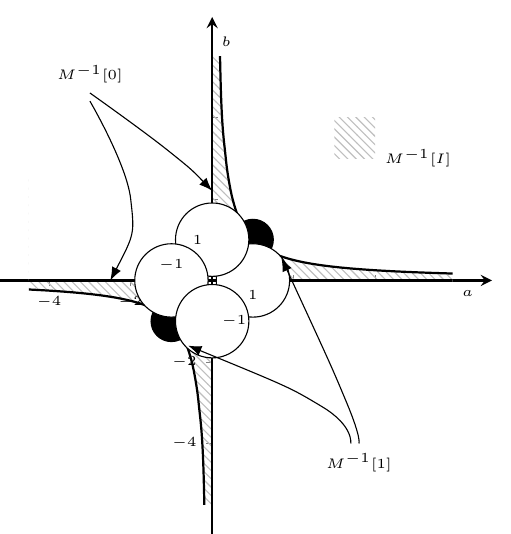
\begin{tikzpicture}
\begin{axis}[ 
xlabel=$a$,
ylabel=$b$,
axis x line=center, xlabel style={anchor=north west},
axis y line=center, ylabel style={anchor=south west},
xmin=-4.5,
xmax=5.9,
ymin=-5.5,
ymax=5.5,
axis line style={thick, shorten > = -0.5cm, shorten < = -0.5cm},
samples=50,
unit vector ratio*=1 1,
font=\tiny
]


\addplot [name path = A,domain=-6:-0.09, thick, smooth]{1/x};
\addplot [name path = B,domain=0.09:6, thick,, smooth]{1/x};
\addplot[pattern=north west lines, pattern color=gray!50]fill between[of=A and B , soft clip={domain=-6:6}];

 \coordinate (At) at (axis cs:0,0) {};
\coordinate (Bt) at (axis cs:6,0) {};
\coordinate (Ct) at (axis cs:6,-6) {};
\coordinate (Dt) at (axis cs:0,-6) {};
\path[fill =white](At)--(Bt)--(Ct)--(Dt);
 \coordinate (A) at (axis cs:0,0) {};
\coordinate (B) at (axis cs:-6,0) {};
\coordinate (C) at (axis cs:-6,6) {};
\coordinate (D) at (axis cs:0,6) {};
\path[fill =white](A)--(B)--(C)--(D);
\draw[thick](axis cs:-6,0)--(axis cs:6,0);
\draw[thick](axis cs:0,-6)--(axis cs:0,6);
\coordinate (H1) at (axis cs:1,1) {};

\coordinate (H1a) at (axis cs:1,0) {};

\coordinate (H1b) at (axis cs:0,1) {};

\draw[dashed] (H1)--(H1b);
\draw[dashed] (H1)--(H1a);
\coordinate (H2) at (axis cs:-1,-1) {};
\draw [fill= black] (H2) circle [radius=0.5];
\coordinate (H2a) at (axis cs:-1,0) {};

\coordinate (H2b) at (axis cs:0,-1) {};
\draw[dashed] (H2)--(H2b);
\draw[dashed] (H2)--(H2a);
\draw [fill= black] (H1) circle [radius=0.5];
\draw [fill= white] (H1a) circle [radius=0.9];
\draw [fill= white] (H1b) circle [radius=0.9];
\draw [fill= white] (H2a) circle [radius=0.9];
\draw [fill= white] (H2b) circle [radius=0.9];
\node[below] at (H1a) {$1$};
\node[left] at (H1b) {$1$};
\node[above] at (H2a) {$-1$};
\node[right] at (H2b) {$-1$};

\draw[Latex-]  plot[smooth, tension=.7] coordinates {(axis cs:-0.59,-1.6) (axis cs:2.7,-3.1) (axis cs:3.4,-4)};
\draw  [Latex-]plot[smooth, tension=.7] coordinates {(axis cs:1.7,0.55) (axis cs:3.3,-3) (axis cs:3.6,-4)};
\node[below] at  (axis cs:3.6,-4) {$M^{-1}[1]$};

\draw[Latex-]  plot[smooth, tension=.7] coordinates {(axis cs:-2.5,0) (axis cs:-2,2) (axis cs:-3,4.4)};
\draw  [Latex-]plot[smooth, tension=.7] coordinates {(axis cs:0,2.2) (axis cs:-1.1,3.2) (axis cs:-3.0,4.6)};
\node[above] at (axis cs:-3.0,4.6) {$M^{-1}[0]$};
\path [pattern=north west lines, pattern color=gray!50](axis cs:3,3)--(axis cs:4,3)--(axis cs:4,4)--(axis cs:3,4)--(axis cs:3,3);
\node[right] at (axis cs:4,3) {$M^{-1}[I]$};
\end{axis};
\end{tikzpicture}
\caption{$\text{Inverse image of } M^{-1}(0),\,M^{-1}(1),\, M^{-1}(I)$}
\label{fig:fig_p8b}
\end{figure}
$$\blacklozenge$$

\subsection{}
\begin{tcolorbox}
Examine carefully the content of Theorem $\mathbf{12.6}$ and your answer to Exercise $4(a)$ and $(b)$. Which seems to have a nicer behaviour on collections of sets, $f$ or $f^{-1}$?
\end{tcolorbox}
Putting aside the notion of 'nicer', we still could put forward that $f^{-1}$ requires less restrictions in order to have certain identities. \\
Take first $\mathbf{12.6}(b)\quad f\left[\bigcap\{A_{\delta}:\delta \in \Delta\}\right]\subset \bigcap\{f[A_{\delta}]:\delta \in \Delta\}$ compared to $\mathbf{12.6}(c^{'})\quad f^{-1}\left[\bigcap\{B_{\lambda}:\lambda \in \Lambda\}\right]= \bigcap\{f^{-1}[B_{\lambda}]:\lambda \in \Lambda\}$. $f^{-1}$ requires no special condition (except for $f$ being a function) in order to have an equality for the intersection of the sets in the collection.\\
Moreover in Exercise $4$, for having the identity $4(a)\quad f[A-B] = f[A]-f[B]$, we need $f$ to be at least an injection while for $4(b)\quad f^{-1}[D-C] = f^{-1}[D]-f^{-1}[C]$ we "only need a$f$ to be a surjection which can be achieved by  restricting the target $Y$ to $D\cup C$.
$$\blacklozenge$$
\newpage

 \section{The restriction of a function}
\subsection{}
\begin{tcolorbox}
Let $f:\mathbb{R}\rightarrow \mathbb{R}$ and $g:\Breal\rightarrow \Breal$ be mappings such that $f(x)=\sin x$ for each $x\in \Breal$ and $g(x)=\sqrt{1-\cos^2 x}$ for each $x\in\Breal$. Find the largest interval of real numbers, $I$, whose left endpoint is $0$ and which satisfies $f|I=g|I$.
\end{tcolorbox}
As $g(x)$ can be expressed as $g(x)=|\sin{x}|$ the condition $f(x)=g(x)$ will only be met in the intervals  $\{[2\pi k,\pi (2k+1)]:k\in \mathbb{P}\cup \{0\}\}$. Putting $k=0$ we get $I=[0,\pi]$.
$$\blacklozenge$$

\subsection{}
\begin{tcolorbox}
Let $f:\mathbb{R}\rightarrow \mathbb{R}$ be defined as follows. For each $x\in \Breal$, let $f(x)=|x-1|$. Let $g:\Breal\rightarrow \Breal$  be defined by and $g(x)=x-1$ for each $x\in\Breal$. Find the largest set $S\subset\Breal$ for which  $f|I=g|I$.
\end{tcolorbox}
\begin{figure}[H]%
    \centering
    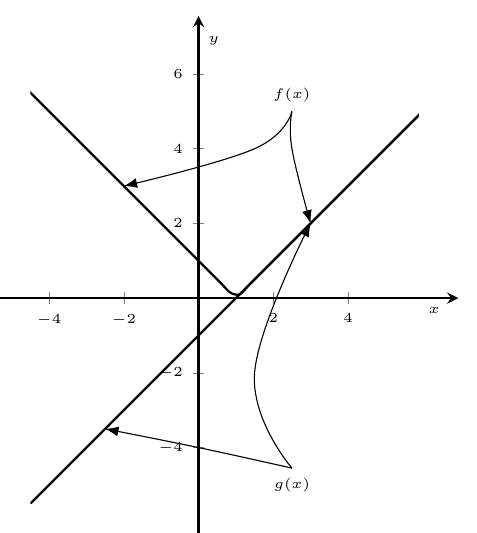
\begin{tikzpicture}
\begin{axis}[ 
xlabel=$x$,
ylabel=$y$,
axis x line=center, xlabel style={anchor=north west},
axis y line=center, ylabel style={anchor=south west},
xmin=-4.5,
xmax=5.9,
ymin=-5.5,
ymax=6.5,
axis line style={thick, shorten > = -0.5cm, shorten < = -0.5cm},
samples=50,
unit vector ratio*=1 1,
font=\tiny
]



\addplot [domain=-6:6, thick, black, smooth]{sqrt((x-1)*(x-1))};
\addplot [domain=-6:6, thick, black, smooth]{x-1};

\draw[-Latex]  plot[smooth, tension=.7] coordinates {(axis cs:2.5,5) (axis cs:2.5,4) (axis cs:3,2)};
\draw[-Latex]  plot[smooth, tension=.7] coordinates {(axis cs:2.5,5) (axis cs:1.5,4) (axis cs:-2,3)};
\node[above] at(axis cs:2.5,5){$f(x)$};

\draw[-Latex]  plot[smooth, tension=.7] coordinates {(axis cs:2.5,-4.55) (axis cs:0,-4) (axis cs:-2.5,-3.5)};
\draw[-Latex]  plot[smooth, tension=.7] coordinates {(axis cs:2.5,-4.55) (axis cs:1.5,-2)  (axis cs:3,2)};
\node[below] at(axis cs:2.5,-4.55){$g(x)$};
\end{axis};
\end{tikzpicture}
\caption{$f(x)=|x-1| \text{ and } g(x)=x-1$}
\label{fig:fig_p8b}
\end{figure}
From the figure we get $S=[1,+\infty)$.
$$\blacklozenge$$

\subsection{}
\begin{tcolorbox}
Let $f:\mathbb{R}\rightarrow \mathbb{R}$ and $g:\Breal\rightarrow \Breal$ be given by $g(x)=\cos x $ and $f(x)=\sqrt{1-\sin^2 x}$ for $x\in \Breal$. Find the largest set $S\subset\Breal$ for which  $f|I=g|I$.
\end{tcolorbox}
As $f(x)\equiv|\cos{x}|$,  $f(x)=g(x)$ implies $S=\{[-\frac{\pi}{2} k,-\frac{\pi}{2}k+\pi]:k\in \mathbb{Z}_{/ \{0\}}\}$.

\newpage
 \section{Composition of functions}
\subsection{}
\begin{tcolorbox}
Let $f:\Breal\rightarrow\Breal$ and $g:\Breal\rightarrow\Breal$ be given by $f(x)= \frac{x}{x+1}$ and $g(x)=x^2$. Give explicit formulas for $g\circ f(x)$ and $f\circ g(x)$. Determine the ranges of $g\circ f$ and $f\circ g$.
\end{tcolorbox}
$$ $$
$g\circ f(x)= \frac{x^2}{x^2+2x+1}$\\
$f\circ g(x)= \frac{x^2}{x^2+1}$\\
$Range \,g\circ f= [0,+\infty)$\\
$Range \,f\circ g=[0,1)$
$$\blacklozenge$$

\subsection{}
\begin{tcolorbox}
Let $f:\Breal\rightarrow\Breal$ and $g:\Breal\rightarrow\Breal$ be defined as follows:
\begin{align*}
\begin{array}{lll}
f(x)&=x^2&\text{for } x\ge 0\\
&=2&\text{for } x< 0\\
g(x)&=\sqrt{x}&\text{for } x\ge 0\\
&=x&\text{for } x<0\\
\end{array}
\end{align*}
(a) Sketch the graph of $g\circ f$\\
(b) Sketch the graph of $f\circ g$\\
(c) Find $\left( f\circ g\right)^{-1}[x]$ for each $x\in \Breal$\\

\end{tcolorbox}
\begin{figure}[H]%
    \centering
  \subfloat[$g\circ f$]{\begin{tikzpicture}[scale=1]
\begin{axis}[ 
xlabel=$x$,
ylabel=$y$,
axis x line=center, xlabel style={anchor=north west},
axis y line=center, ylabel style={anchor=south west},
xmin=-4.5,
xmax=5.9,
ymin=-5.5,
ymax=6.5,
axis line style={thick, shorten > = -0.5cm, shorten < = -0.5cm},
samples=50,
unit vector ratio*=1 1,
font=\tiny
]
\addplot [domain=0:6, ultra thick, black, smooth]{x};
\addplot [domain=-6:0, ultra thick, black, smooth]{sqrt(2)};
\draw [fill= white] (axis cs:0,1.4142136) circle [radius=10.05];
\node[right] at (axis cs:0,1.4142136) {$\sqrt{2}$};
\end{axis};
\end{tikzpicture}}\quad
    \subfloat[$f\circ g$]{\begin{tikzpicture}[scale=1]
\begin{axis}[ 
xlabel=$x$,
ylabel=$y$,
axis x line=center, xlabel style={anchor=north west},
axis y line=center, ylabel style={anchor=south west},
xmin=-4.5,
xmax=5.9,
ymin=-5.5,
ymax=6.5,
axis line style={thick, shorten > = -0.5cm, shorten < = -0.5cm},
samples=50,
unit vector ratio*=1 1,
font=\tiny
]



\addplot [domain=0:6, ultra thick, black, smooth]{x};
\addplot [domain=-6:0, ultra thick, black, smooth]{2};
\draw [fill= white] (axis cs:0,2) circle [radius=10.05];
\node[right] at (axis cs:0,2) {${2}$};
\end{axis};
\end{tikzpicture}}
    %\caption{}
\label{fig:fig_p3}
\end{figure}
(c) Find $\left( f\circ g\right)^{-1}[x]$ for each $x\in \Breal$\\\\
$\left( f\circ g\right)^{-1}[x]=\emptyset, \forall x< 0$\\\\
$\left( f\circ g\right)^{-1}[x]=\{x\}, \forall x\ge 0$\\\\
$\left( f\circ g\right)^{-1}[x]=(-\infty,0)\cup \{{2}\} \text{ for } x= {2}$
$$\blacklozenge$$

\subsection{}
\begin{tcolorbox}
Let $f:\Breal\rightarrow\Breal$ and $g:\Breal\rightarrow\Breal$ be given by $f(x)=\sin{x}$ and $g(x)= |x|$. Write explicit expressions for $g\circ f(x)$ and $f\circ g(x)$ and find the range of each.
\end{tcolorbox}
$$ $$ 
$g\circ f(x)= |\sin{x}|$\\
$f\circ g(x)= \sin{|x|}$\\
$Range \,g\circ f= [0,1]$\\
$Range \,f\circ g=[-1,1]$
$$\blacklozenge$$

\subsection{}
\begin{tcolorbox}
Let $f:\Breal\rightarrow\Breal$ and $g:\Breal\rightarrow\Breal$ be given by $f(x)=x^2+2$ and $g(x)= x-1$. Find expressions for $(g\circ f)(x)$ and $(f\circ g)(x)$ and note that $g\circ f\ne f\circ g$.
\end{tcolorbox}
$$ $$ 
$(g\circ f)(x)=x^2+1$\\
$(f\circ g)(x)= x^2-2x+3$\\
$$\blacklozenge$$
\newpage

\subsection{}
\begin{tcolorbox}
Let $f:\Breal\rightarrow\Breal$,$g:\Breal\rightarrow\Breal$  and $h:\Breal\rightarrow\Breal$ be given by $f(x)=x^2+x$, $g(x)=(x-1)^2$  and $h(x)= x+1$ for each $x\in\Breal$. Find an expression for $h\circ g\circ f(x)$ for $x\in\Breal$.
\end{tcolorbox}
$$ $$ 
 $h\circ g\circ f(x)=\underbrace{ \underbrace{\left((\underbrace{x^2+x}_{f(x)})-1\right)^2}_{g(x)}+1}_{h(x)}=x^4+2x^3-x^2+2x+2$
$$\blacklozenge$$


\subsection{}
\begin{tcolorbox}
Suppose $f:X\rightarrow Y$ is a bijection. Show that $f^{-1}\circ f=i$ where $i:X\rightarrow X$ is the identity map on $X$ and $f\circ f^{-1}=j$ where $j$ is the identity map on $Y$.
\end{tcolorbox}
$$ $$ 
$\mathbf{f^{-1}\circ f=i}$\\
Let $x\in X$. Then, $\left(x,f(x)\right) \in f$. Hence, $\left(f(x),x\right) \in f^{-1}$. thus, $f^{-1}\left(f(x)\right)= x$ and $\left(f^{-1}\circ f\right)(x)= x$ for each $x\in X$. hence, $f{-1}\circ f = i$, the identity map on $ X$. \\
$\mathbf{f=i\circ f^{-1}=j}$\\
Let $y\in Y$. Then, $\left(y,f^{-1}(y)\right) \in f^{-1}$. Hence, $\left(f^{-1}(y),y\right) \in f$. thus, $f\left(f^{-1}(y)\right)= y$ and $\left(f\circ f^{-1}\right)(y)= y$ for each $y\in Y$. hence, $f\circ f^{-1} = j$, the identity map on $ Y$.\\
Note that in the step  \textit{$\left(y,f^{-1}(y)\right) \in f^{-1}$} we implicitly use the fact that $f$ is a bijection.
 
$$\blacklozenge$$

\subsection{}
\begin{tcolorbox}
Let $f:\Breal\rightarrow\Breal$ and $g:\Breal\rightarrow\Breal$ be surjections. Suppose $g\circ f=i$ where $i:X\rightarrow X$ is the identity map on $X$. Show: 
\begin{align*}
\begin{array}{ll}
(a)&f\text{ is one-to-one}\\
(b)&g\text{ is one-to-one}\\
(c)&f\circ g = j \text{ where } j:X\rightarrow X \text{ is the identity map from} $Y$ \text{ onto }$Y$\\
(d)&f=g^{-1}\\
(d)&g=f^{-1}
\end{array}
\end{align*}

\end{tcolorbox}
$$ $$ 
(a) $\mathbf{f\text{ is one-to-one}}$\\
Suppose that $f$ is not one-to-one. This means that there exist $2$ or more $x_1,x_2,\dots $ which are mapped by $f$ to an element $y^{*}\in Y$. But as $g$ is a function, the image $g[\{y^{*}\}]$ can only have one element. Hence, $x_1$ or $x_2$ will not be included in this image. Suppose that $x_2$ is not an element of $g[\{y^{*}\}]$. As $g$ is a surjection, there must be an $y^{'}\in Y$ so that $g(y^{'})= x_2$. But also $f$ is a surjection, so there must be an $x_3\in X$ so that $f(x_3)= y^{'}$. 
So $g(y^{'})= x_2$ implies $g(f(x_3))= x_2$. But $g(f(x_3))= g\circ f(x^3)$ and given that $g\circ f=i$ (the identity map) we get $g\circ f(x^3)=x_3$ and can conclude that $x_2=x_3$ resulting in $f(x_2)= y^{'}$. But we started with the assumption that $f(x_2)= y^{*}$ and as $f$ is a function, this means $y^{'}=y^{*}$, so there is no other $(y,x_2)\in g$ that maps $y$ to $x_2$, meaning that only the element $x_1$ is mapped to the chosen $y^{*}$. Hence $f$ is one-to-one.
$$\lozenge$$

(b) $\mathbf{g\text{ is one-to-one}}$\\
Suppose that $g$ is not one-to-one. This means that for a given $x^{*} $ we could have $2$ (or more) $y_1,y_2,\dots$, so that $g(y_1)=x^{*}$ and $g(y_2)=x^{*}$. But $f$ is on-to-one (see $1.14.7 (a)$) so we must have two distinct $x_1,x_2$ for which we have $f(x_1)=y_1$ and $f(x_2)=y_2$, but $g(y_1)=x^{*}$ and $g(y_2)=x^{*}$, so $g\circ f(x_1)=x^{*}$ and $g\circ f(x_2)=x^{*}$ and given that $g\circ f=i$ (the identity map) we get $x_1=x_2=x^{*}$ and also $y_1=y_2$ and conclude that $g$ must be one-to-one.
$$\lozenge$$

(c) $\mathbf{f\circ g = j \text{ where } j:X\rightarrow X \text{ is the identity map from } Y \text{ onto }Y}$\\
We have $g\circ f=i$, so $g\circ f(x)=x$. As $x\in X$ we can apply $f$ to $x$ and this gives $(f\circ g\circ f)(x)=f(x)$ or $(f\circ g)\circ f(x)=f(x)$. Put $f(x)=y$, we can rewrite this as $(f\circ g)(y)=y$. Hence $f\circ g$ is the identity map $j:Y\rightarrow Y$.
$$\lozenge$$


(d) $\mathbf{f=g^{-1}}$\\
Be $(y,x)\in g$. Then, $(x,y)\in g^{-1}$. As $f$ is a bijection, we have one $x\in X$ and one $y\in Y$ so that $y= f(x)$. Then, $(x,y)\in g^{-1}$ is equivalent to $(x,f(x))\in g^{-1}$. But, by definition , we have  $(x,f(x))\in f$, and conclude $f\subset g^{-1}$. \\
Be now, $(x,y)\in f$. As $g$ is one-to-one (see above), there is just one $(x,y)$ so that $x=g(y)$. Thus, $(g(y),y)\in f$. We notice that $(y, g(y))\in g$, or $(g(y),y )\in g^{-1}$. This give with $(g(y),y)\in f$, $g^{-1}\subset f$.\\
Combining with the first subset we get $f=g^{-1}$.
$$\lozenge$$
(e) $\mathbf{g=f^{-1}}$\\
Be $(x,y)\in f$. Then, $(y,x)\in f^{-1}$. As $g$ is a bijection, we have one $x\in X$ and one $y\in Y$ so that $x= g(y)$. Then, $(y,x)\in f^{-1}$is equivalent to $(y,g(y))\in f^{-1}$. But, by definition , we have  $(y,g(y))\in g$, and conclude $g\subset f^{-1}$. \\
Be now, $(y,x)\in g$. As $g$ is one-to-one (see above), there is just one $(y,x)$ so that $x=g(y)$. Thus, $(y,g(y))\in g$. But $y=f(x)$.  This gives  $(f(x),\underbrace {f\circ g}_{=j}(y))\in g$. But we notice that $(x,f(x))\in f $ or  $(f(x),x)\in f^{-1} $ and conclude with $(f(x),x)\in g$ that  $f^{-1}\subset g$.\\
Combining with the first subset we get $g=f^{-1}$.
$$\blacklozenge$$
\subsection{}
\begin{tcolorbox}
Recall that $\Breal_{+}=\left\{x:x\in \Breal \text{ and } x> 0\right\}$. Recall also that the natural logarithm function , $\ln$, is defined on $\Breal_{+}$, with range $\Breal$; the exponential function, $ \{(x,e^x):x\in \Breal\}$, is the inverse of the of the $\ln$ function.; $\cosh x = \frac{ e^x+e^{-x}}{2}$ for each $x\in \Breal$. \\
Sketch the $\cosh$ function and note that although $\cosh$ is not one-to-one, the restriction $\cosh |\Breal_{+}$ is one-to-one and hence, its inverse is a function. By using the results of  Exercise $1.14.7$, prove that $\cosh^{-1}(x)= \ln \left(x+\sqrt{x^2-1}\right)$ for $x\ge 1$.
\end{tcolorbox}
$$ $$ 
\begin{figure}[H]%
    \centering
    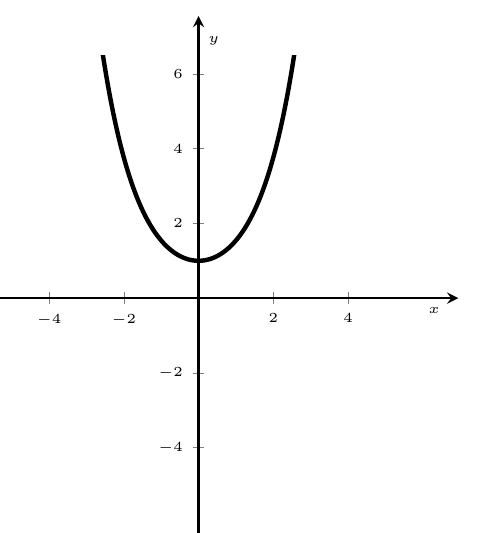
\begin{tikzpicture}
\begin{axis}[ 
xlabel=$x$,
ylabel=$y$,
axis x line=center, xlabel style={anchor=north west},
axis y line=center, ylabel style={anchor=south west},
xmin=-4.5,
xmax=5.9,
ymin=-5.5,
ymax=6.5,
axis line style={thick, shorten > = -0.5cm, shorten < = -0.5cm},
samples=50,
unit vector ratio*=1 1,
font=\tiny
]

\addplot [domain=-3:3, ultra thick, black, smooth]{(exp(x)+exp(-x))*0.5};

\end{axis};
\end{tikzpicture}
\caption{The function $\cosh x$}
\label{fig:fig_p8b}
\end{figure}
For two functions $f:\Breal\rightarrow\Breal$ and $g:\Breal\rightarrow\Breal$ for which yields $g\circ f=i$, we know from Exercise $1.14.7(c)$  that  $f\circ g=j$ (the unit map). We put  $f(x)= \cosh x = \frac{ e^x+e^{-x}}{2}$ and try to find $g= f^{-1}$. From the sketch, we see that if we restrict $x$ to $[0,+\infty)$ that $f$ is bijective with $Range\, f= [1,+\infty)$. \\
What we have to do, is to solve the functional equation $g\left(\frac{ e^x+e^{-x}}{2}\right)=x$ (with $g=f^{-1}$) (this expression represent $g\circ f=i$).\\
We use the identity $a=e^{\ln a}$ and use the equivalence of  $g\circ f=i$ and $f\circ g=j$, i.e. $$\frac{ e^{g(y(}+e^{-g(y)}}{2} =y$$
 We put tentatively $g(y) = \ln p(y)$ with $p: [1,+\infty)\rightarrow\Breal$ and get from $a=e^{\ln a}$:
 \begin{align*}
 &\frac{ e^{g(y)}+e^{-g(y)}}{2} =y\\
 \Leftrightarrow \quad &\frac{ e^{\ln p(y)}+e^{-g(y)}}{2} =y\\
 \Leftrightarrow \quad &\frac{ p(y)+\frac{1}{p(y)}}{2} =y\\
 \Leftrightarrow \quad &p^2(y)-2 p(y)y  =-1\\
 \Leftrightarrow \quad &p^2(y)-2 p(y)y+y^2  =y^2-1\\
 \Leftrightarrow \quad &\left(p(y)-y\right)^2  =y^2-1\\
 \Rightarrow \quad &p(y)= y\pm \sqrt{y^2-1}\\
 \end{align*}
 From our definition $g(y) = \ln p(y)$, we get $g(y) = \ln \left(y\pm \sqrt{y^2-1}\right)$. To get a real valued $g$ we need obviously $y\ge 1$ but also need that $g(y)\ge 0$ as we restricted the function $f$ to $\Breal_{+}$ which requires $y\pm \sqrt{y^2-1}\ge 1$ and thus only the solution $g(y) = \ln \left(y+ \sqrt{y^2-1}\right),\quad y\ge 1$ can be retained.
$$\blacklozenge$$

\subsection{}
\begin{tcolorbox}
Consider the map $P:\Breal^2\rightarrow \Breal$ such that for each $(x,y)\in \Breal^2$, $\alpha\left((x,y)\right)$ is the element $(u,v)\in \Breal^2$ given by $u=2x-y,\, v= 5x+y$. Recall that $\Breal^2$ denotes $\Breal\times\Breal$.\\
\begin{align*}
\begin{array}{ll}
(a)&\text{Does }\alpha[\Breal^2] = \Breal^2\text{ ?}.\\
(b)&\text{Is }\alpha\text{ one-to-one?}.\\
(c)&\text{If }\alpha\text{ is one-to-one, find a rule for }\\
&\alpha^{-1} \text{ analogous to the rule given for }\alpha.
\end{array}
\end{align*} 
\end{tcolorbox}
$$ $$ 
(a)$ \text{ Does }\alpha[\Breal^2] = \Breal^2\text{ ?}$\\
(b)$\text{Is }\alpha\text{ one-to-one?}$.\\
The answer is yes to both questions as we can consider the map as a system of linear equation with $(x,y)$ as unknowns and $(u,v)$ as parameters i.e.
\begin{align*}
\left\{\begin{matrix}
2x-y=u\\ 5x+y=v
\end{matrix}\right.
\end{align*}
 The determinant of this system is not zero (it is $7$) and so for every $(u,v)$ we have a unique $(x,y)$. From the definition it is also clear that $u,v\in \Breal$ (it is in fact a map from one plane to another plane).\\
  So, $\alpha[\Breal^2] = \Breal^2$ and $\alpha$ is a bijection.
  $$\lozenge$$
 (c) If $\alpha$ is one-to-one, find a rule for $\alpha^{-1}$  analogous to the rule given for $\alpha$.
 \begin{align*}
\left\{\begin{matrix}
x=& \frac{u+v}{7}\\ y=& \frac{2v-5u}{7}
\end{matrix}\right.
\end{align*}

$$\blacklozenge$$

\subsection{}
\begin{tcolorbox}
Consider the map $P:\Breal^2\rightarrow \Breal$ such that for each $(x,y)\in \Breal^2$, $P\left((x,y)\right)=x$. Note that $P$ is not one-to-one. Find a subset $S$ of $\Breal^2$ such that $P | S:S\rightarrow \Breal$ is a one-to-one map from $S$ to $\Breal$.
\end{tcolorbox}
$$ $$ 
We can find two types of restrictions:\\
A type with $y$ a constant i.e. $P_r | S_r:S_r\rightarrow \Breal$ with $P_r=\{(x,r): x\in\Breal,\, r\in \Breal = \text{ constant}\}$.\\

And a type with $y= f(x)$ where $f:\Breal\rightarrow \Breal$ is a one-to-one function.
 
$$\blacklozenge$$

\subsection{}
\begin{tcolorbox}
Suppose $f: A\rightarrow B$ is a one-to-one map from $A$ to $B$ and $g:B\rightarrow C$ is a one-to-one map from $B$ into $C$. Prove that $g\circ f:A\rightarrow C$ is one-to-one map from $A$ into $C$.
\end{tcolorbox}
Suppose $g\circ f$ is not one-to-one. This means that for at least one $z\in C$ there exist two (or more) $x_1,\, x_2$ such that $(x_1,z^{*})\text{ and } (x_2,z^{*})\in g\circ f$. But $f: A\rightarrow B$ and $g:B\rightarrow C$ are one-to-one maps which means that $x_1\in A$ is mapped to a unique $y_1\in B$ (the same for  $x_2$ mapped to a unique $y_2$) and also $y_1\in B$ is mapped to a unique $z_1\in C$ (the same for $y_2$ mapped to a unique $z_2$). So the map $ g\circ f$ will map $x_1$ into $z_1$ and $x_2$ into $z_2$. So supposition that there exist a $z^{*}$ is in contradiction with our result that $z_1\ne z_2$. \\
Is $g\circ f$ a surjection ?\\
As $f$ and $g$ are one-to-one, every $y\in B$ and every $z\in C$ are covered by $f,g$ respectively, so every $z\in C$ is also covered by $g\circ f$. So, $g\circ f$ is a surjection and by the first argument also a bijection. 
$$ $$ 

 
$$\blacklozenge$$


\subsection{}
\begin{tcolorbox}
Let $f:\Breal\rightarrow \Breal$ be a map such that for each pair of numbers $x$ and $y$, $f(x+y)=f(x)+f(y)$. 
\begin{align*}
\begin{array}{ll}
(a)&\text{Show that  }f(0)=0.\\
(b)&\text{Show that  }f(-x)=-f(x),\quad\forall x\in \Breal.\\
(c)&\text{Show that  }f(mx)=mf(x),\quad \forall m \in \mathbb{Z}, x\in \Breal.\\
(d)&\text{Show that  }f(rx)=rf(x),\quad \forall r \in \mathbb{Q}, x\in \Breal.\\
\end{array}
\end{align*} 
\end{tcolorbox}
$$ $$ 
(a) Show that $f(0)=0$.\\
Put $x=0$ and $y=0$. We have, $\underbrace{f(0+0)}_{=f(0)} =\underbrace{f(0)+f(0)}_{=2f(0)}$. This implies that $f(0)=0$.\\\\
(b) Show that $f(-x)=-f(x),\quad\forall x\in \Breal$.\\
Put  $y=-x$. We have, $\underbrace{f(x+(-x))}_{=f(0)=0} =f(x)+f(-x)$. This implies that $f(-x)=-f(x)$.\\\\
(c) Show that $f(mx)=mf(x),\quad \forall m \in \mathbb{Z}, x\in \Breal$.
\begin{align*}
f(mx)&= f(x+ (m-1)x)\\
&= f(x)+ f((m-1)x)\\
&= f(x)+ f(x+(m-2)x)\\
&= f(x)+ f(x)+f((m-2)x)\\
&=\quad \vdots\\
&= \underbrace{f(x)+ f(x)+\dots f(x)}_{=mf(x)}
\end{align*}
and get the required result.\\
(d) Show that $f(rx)=rf(x),\quad \forall r \in \mathbb{Q}, x\in \Breal$.
\begin{align*}\begin{matrix}
&f(rx)&= f(\frac{m}{n}x)\\
\Leftrightarrow& f(rx)&= mf(\frac{1}{n}x)\\
\times n\quad & nf(rx)&= mnf(\frac{1}{n}x)\\
\Leftrightarrow&nf(rx) &= mf(\frac{n}{n}x)\\
\Rightarrow & f(rx) &= \frac{m}{n}f(x)\\
\Rightarrow & f(rx) &= rf(x)
\end{matrix}
\end{align*}
 
$$\blacklozenge$$
\newpage
 \section{Sequences}
\subsection{}
\begin{tcolorbox}
In each of the following find a formula for the $n$th term $a_n$ of an infinite sequence whose first five terms are given. 
\begin{align*}
\begin{matrix}
(a)& a_l = 1, a_2 = \frac{1}{2}, a_3 = \frac{1}{4}, a_4 = \frac{1}{8}, a_5 =\frac{1}{16} \\
(b)& a_1= 1, a_2 = 0, a_3= 1, a_4= 0, a_5 = 1. \\
(c)& a_1= 1 , a_2 = 0, a_3= -1, a_4= 0, a_5 = 1. \\
(d)& a_1= 1, a_2 = 3, a_3= 6, a_4= 10, a_5 = 15. \\ 
\end{matrix}
\end{align*}
\end{tcolorbox}
$$ $$
(a) $ a_l = 1, a_2 = \frac{1}{2}, a_3 = \frac{1}{4}, a_4 = \frac{1}{8}, a_5 =\frac{1}{16}$ \\
$$a_n=\frac{1}{2^{n-1}}$$
$$\lozenge$$
(b) $ a_1= 1, a_2 = 0, a_3= 1, a_4= 0, a_5 = 1$ \\
$$a_n=n\Mod{2}$$
$$\lozenge$$
(c) $ a_1= 1 , a_2 = 0, a_3= -1, a_4= 0, a_5 = 1$ \\
$$a_n=\left(\sin \frac{\pi}{2}n\right)\left(n\Mod{2}\right)$$
$$\lozenge$$
(d) $ a_1= 1, a_2 = 3, a_3= 6, a_4= 10, a_5 = 15$ \\
$$a_{n+1}=a_{n}+ (n+1),\quad a_1=1$$

$$\blacklozenge$$

\subsection{}
\begin{tcolorbox}
Let $f= (f_i)_{i=1}^{+\infty}$  g, be the sequence defined as follows: Let $g(x) = \sin x$. For each positive integer $i$, let $f_i = g^{(i)}(0)$, where $g^{(i)}$ is the $i^{th}$ derivative of $g$. Write the terms off sufficiently far to see the pattern followed.
\end{tcolorbox}
$$ $$
We have $g^{(1)}(x)=\cos x,\,g^{(2)}(x)=-\sin x,\,g^{(3)}(x)=-\cos x,\,g^{(4)}(x)=\sin x,\,g^{(5)}(x)=\cos x,\,\dots$, so we get $f=(1,0,-1,0,1,0,-1,\dots$, so from Exercise $1.15.1(c)$, we get
$$f_i=\left(\sin \frac{\pi}{2}i\right)\left(i\Mod{2}\right)$$
$$\blacklozenge$$
\\
\subsection{}
\begin{tcolorbox}
For each $n \in P$ , let $a_n = \sum_{j=1}^{n}j^2$. Try to discover a formula for $a_n$.
\end{tcolorbox}
$$ $$
We can suppose that when $n\rightarrow +\infty$ that $a_n = \sum_{j=1}^{n}j^2$ and $\int_0^{n}x^2dx$ will tend to a common value. As $\int_0^{n}x^2dx= \frac{1}{3}n^3$ we tentatively write $a_n$ as a cubic expression $a_n= an^3+bn^2+cn+d$. As $a_{n+1} = a_n +(n+1)^2$ we try to find the parameters $a,\,b,\,c,\,d $ by solving the expression $$ a(n+1)^3+b(n+1)^2+c(n+1)+d =  an^3+bn^2+cn+d+ (n+1)^2$$
for some values of $n$.
Expanding gives $$(3a-1)n^2+(3a+2b-2)n+a+b+c-1=0 $$
For $n=1,2,3$ we get the following system of linear equations
\begin{align*}
\left\{
\begin{array}{l}
7a+3b+c=4\\
19a+5b+c=9\\
37a+7b+c=16
\end{array}
\right.
\end{align*}
and get $a_n=\frac{1}{3},\, b= \half,\, c= \frac{1}{6}$ giving
$a_n= \frac{1}{3}n^3+\half n^2+\frac{1}{6}n+d$ and for $n=1,\, a_n=1$ we get $1= \underbrace{\frac{1}{3}+\half+\frac{1}{6}}_{=1}+d$, giving $d=0$.
So, we get the expression $a_n= \frac{1}{3}n^3+\half n^2+\frac{1}{6}n$ which can be rewritten as 
$$ a_n= \frac{n(2n+1)(n+1)}{6}$$ 
Yet, we didn't prove formally that this equation works for every $n$:\\
We notice that this equation is exact for $n=1$. Suppose that it is also correct for a $n$. Then:\\
\begin{align*}
a_{n+1}&= a_{n} + (n+1)^2\\
&=  \frac{1}{3}n^3+\half n^2+\frac{1}{6}n + (n+1)^2\\
&=  \frac{1}{3}n^3+\half n^2+\frac{1}{6}n + n^2+2n+1\\
&=  \frac{1}{3}n^3+\frac{3}{2}n^2+\frac{13}{6}n+1\\
\end{align*}
Using the proposed closed expression for $n+1$ gives
\begin{align*}
a_{n+1}&=\frac{1}{3}(n+1)^3+\half (n+1)^2+\frac{1}{6}(n+1)\\
&=\frac{1}{3}n^3+n^2+n+\frac{1}{3}+\half n^2+n+\half+\frac{1}{6}n+\frac{1}{6}\\
&=\frac{1}{3}n^3+\frac{3}{2}n^2+\frac{13}{6}n+1\\
\end{align*}
So, both expression are the same and by the axiom of induction , we conclude that the expression is correct for every $n$.

$$\blacklozenge$$

\subsection{}
\begin{tcolorbox}
Suppose that $a$ is a sequence such that $a_l = 1,\, a_2 = 3,\, a_3 = a_1+a_2,$ and for $j \ge 3,\, a_j = a_{j-1}+a_{j-2}$. Find $a_4,\, a_5,\, a_6$ and $a_7$.
\end{tcolorbox}
$$ $$
$a_4=6,\,a_5=10,\,a_6=16,\,a_7=26$.
$$\blacklozenge$$

\subsection{}
\begin{tcolorbox}
Suppose a sequence a is given by $a_n = 2^n$ for each positive integer $n$. For which values of $n$ is it true that $a_n\ge 10,000$?
\end{tcolorbox}
$$ $$
We have to find a $n$ such that $\log_2 2^n \ge \log_2 10,000$ (the logarithm function is a strict increasing function). \\
So, $n\ge \log_{10} 10,000 \log_2 10$ or $n\ge \underbrace{4\times 3.3}_{=13.3}$ and hence $n\ge 14$.
$$\blacklozenge$$

\subsection{}
\begin{tcolorbox}
Let a be the sequence given by $a_n = \frac{n}{ (n + 1)}$. Find the smallest integer $N$ such that for $n\ge N,\, a_n > \frac{9}{10}$.
\end{tcolorbox}
$$ $$
We need $\frac{n}{ (n + 1) }> \frac{9}{10}$ or $n> 9$, hence $N=10$.
$$\blacklozenge$$

\subsection{}
\begin{tcolorbox}
Let a be the sequence given by $a_n= \sqrt{n+1} -\sqrt{n}$. Find an integer $N$ such that for $n\ge  N,\, a_{n+1} < a_n$. Find an integer $M$ such that for $n\ge M, \, a_n\le \frac{1}{10}$.
\end{tcolorbox}
$$ $$
$a_{n+1} < a_n$ gives $\sqrt{n+1} -\sqrt{n} < \sqrt{n} -\sqrt{n-1}$ or $\sqrt{n+1}+\sqrt{n-1} < 2\sqrt{n} $. As both sides are positive, we can take the power of thus inequality and get $2n+2\sqrt{n^2-1} < 4n $ or $\sqrt{n^2-1} < n $ giving the trivial inequality $0> -1$ meaning that the inequality yields for all $N>0$.\\\\
$a_n\le \frac{1}{10}$\\
We have 
\begin{align*}
&\sqrt{n+1} -\sqrt{n}\le \frac{1}{10}\\
\Rightarrow\quad & n+1\le \left(\sqrt{n}+ \frac{1}{10}\right)^2\\
\Rightarrow\quad & (4.95)^2 \le n\\
\end{align*}
from which we conclude that $n$ must be greater or equal to $25$.
$$\blacklozenge$$

\subsection{}
\begin{tcolorbox}
For each $(x, y)\in \Breal^2$, let $f(x, y) = (x^2 -y^2, 2xy)$. Let the point $p_1$ in the plane be given by $f(\half,\half),\, p_2 = f(p_1),\, p_3 = f(p_2),\, p_4= f(p_3),\, p_5 = f(p_4)$. Calculate and plot the points $p_1,\, p_2,\,\dots,\,p_5$.
\end{tcolorbox}
$$ $$
$p(1)=(0,\half), \,p(2)=(-\frac{1}{2^2},0), \,p(3)=(\frac{1}{2^4},0), \,p(4)=(\frac{1}{2^8},0), \,p(5)=(\frac{1}{2^{16}},0)$\\ 
\begin{figure}[H]%
    \centering
    \begin{tikzpicture}[spy using outlines={circle, magnification=4, size=6cm, connect spies}]
\begin{axis}[ 
xlabel=$x$,
ylabel=$y$,
axis x line=center, xlabel style={anchor=north west},
axis y line=center, ylabel style={anchor=south west},
xmin=-0.3,
xmax=0.55,
ymin=-0.05,
ymax=0.6,
axis line style={thick, shorten > = -0.5cm, shorten < = -0.5cm},
samples=50,
unit vector ratio*=1 1,
font=\tiny
]

\coordinate (p0) at (axis cs:0.5,0.5);
\draw [fill= black] (p0) circle [radius=10.05];
\node[right] at (p0) {$p_0$};

\coordinate (p1) at (axis cs:0,0.5);
\draw [fill= white] (p1) circle [radius=10.05];
\node[right] at (p1) {$p_1$};

\coordinate (p2) at (axis cs:-1/2/2,0);
\draw [fill= white] (p2) circle [radius=10.05];
\node[above] at (p2) {$p2$};

\coordinate (p3) at (axis cs:1/2/2/2/2,0);
\draw [fill= white] (p3) circle [radius=10.05];
\node[above ] at (p3) {$p_3$};

\coordinate (p4) at (axis cs:1/2/2/2/2/2/2/2/2,0);
\draw [fill= white] (p4) circle [radius=10.05];
\node[anchor = north west] at (p4) {$p_4$};

\coordinate (p5) at (axis cs:1/2/2/2/2/2/2/2/2/2/2/2/2/2/2/2/2,0);
\draw [fill= white] (p5) circle [radius=10.05];
\node[above left] at (p5) {$p_5$};
\coordinate (a) at (axis cs:0,0);
\end{axis};
\spy [dashed] on (a) in node  at (-2,4);
\end{tikzpicture}
\caption{The dynamical system $f(x, y) = (x^2 -y^2, 2xy)$ with starting point $(\half,\half)$}
\label{fig:fig_p8b}
\end{figure}
$$\blacklozenge$$

\subsection{}
\begin{tcolorbox}
Let $A_l = \{1, 2, 3\}, A_2 = \{1, 2\}, A_3 = \{a,b\}$.  Write out the elements of $A_1 \times A_2\times A_3$. Write out the elements of $(A_1\times A_2) \times A_3$. Show that there is a "natural" one-to-one correspondence between the elements of these two sets. 
\end{tcolorbox}
$$ $$
$A_1 \times A_2\times A_3$\\
\begin{align*}
\left\{\begin{matrix}
(1, 1, a)&(1, 1, b)&(1, 2, a)&(1, 2, b)\\
(2, 1, a)&(2, 1, b)&(2, 2, a)&(2, 2, b)\\
(3, 1, a)&(3, 1, b)&(3, 2, a)&(3, 2, b)\\
\end{matrix}
\right\}
\end{align*}

$\left(A_1 \times A_2\right)\times A_3$\\
\begin{align*}
\left\{\begin{matrix}
\left((1, 1), a\right)&\left((1, 1), b\right)&\left((1, 2), a\right)&\left((1, 2), b\right)\\
\left((2, 1), a\right)&\left((2, 1), b\right)&\left((2, 2), a\right)&\left((2, 2), b\right)\\
\left((3, 1), a\right)&\left((3, 1), b\right)&\left((3, 2), a\right)&\left((3, 2), b\right)\\
\end{matrix}
\right\}
\end{align*}
As the two sets have the same number of elements, we can define a bijection between the two sets. The most natural bijection is the one which maps an element $(x,y,z)\in A_1 \times A_2\times A_3$ to $\left((x,y),z\right)\in \left(A_1 \times A_2\right)\times A_3$ according to the following scheme:
\begin{figure}[H]%
    \centering
    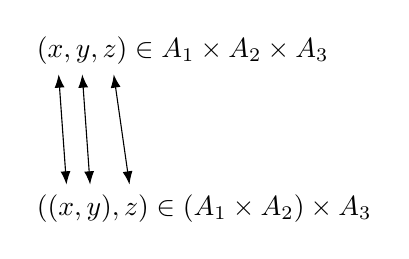
\begin{tikzpicture}
\coordinate (set1) at (0,0);
\node[right] at (set1) {$(x,y,z)\in A_1\times A_2\times A_3$};

\coordinate (set2) at (0,-2);
\node[right] at (set2) {$\left((x,y),z\right)\in \left(A_1\times A_2\right)\times A_3$};



\node at (1.1,-0.3) {};
\node at (1.3,-1.7) {};
\draw[Latex-Latex] (0.4,-0.3)-- (0.5,-1.7) ;
\draw[Latex-Latex]  (1.3,-1.7)-- (1.1,-0.3) ;
\draw[Latex-Latex] (0.7,-0.3)-- (0.8,-1.7) ;

\end{tikzpicture}
\caption{"natural" one-to-one correspondence between the elements of $A_1 \times A_2\times A_3$ and $(A_1\times A_2) \times A_3$}
\label{fig:fig_p8b}
\end{figure}
$$\blacklozenge$$

\subsection{}
\begin{tcolorbox}
Suppose that for each $i \in  \mathbb{P},\, A_i = \{0, \,1\}$. Describe in words the set $\bigtimes\{A_i:i \in \mathbb{P}\}$.
\end{tcolorbox}
$$ $$
Each element of $\bigtimes\{A_i:i \in \mathbb{P}\}$ is of the form $(1,0,0,\dots, 1,1\dots 0,1\dots)$ and can be interpreted as the binary representation of any $n\in \mathbb{P}\cup\{0\}$. (In the given example $n= 1\times 2^0+0\times 2^1+0\times 2^2+\dots+ 1\times 2^k +1\times 2^{k+1}+\dots + 0\times 2^p + 1\times 2^{p+1}+\dots$).
$$\blacklozenge$$

\subsection{}
\begin{tcolorbox}
Let $A_1$ be the set of all real numbers $\Breal$. For each $i \in \mathbb{P}$ such that $i \ge 2$, let $A_i=\{0\}$. Describe in words the set $\bigtimes \{A_i: i \in \mathbb{P}\}$. Show that there exists a bijection from $\bigtimes \{A_i: i \in \mathbb{P}\}$ onto $\Breal$.
\end{tcolorbox}
$$ $$
Each element of $\bigtimes\{A_i:i \in \mathbb{P}\}$ is of the form $(r,0,0,0,\dots),\, r\in \Breal$ and can be interpreted in different ways. One way is to consider an element of $\bigtimes\{A_i:i \in \mathbb{P}\}$ as the coordinates of a family of points in an infinite dimensional vector space where the points are strictly collinear with the first base vector.\\
The bijection is trivial as for each point of this family, only one real number is assigned along the first base vector
$$\blacklozenge$$

\newpage

 \section{Sequences and Subsequences}
\subsection{}
\begin{tcolorbox}
Consider the sequence $S = (1,\half,\frac{1}{3},\dots,\frac{1}{n },\dots)$. Find a map $N:\mathbb{P}\rightarrow \mathbb{P}$ such that $S\circ N$  is the sequence $(\frac{1}{3}, \frac{1}{6},\dots , \frac{1}{3n},\dots )$. 
\end{tcolorbox}
$$ $$
Define the  map $N:\mathbb{P}\rightarrow \mathbb{P}$ as $N=\{n,3n):n\in\mathbb{P}\}$.
$$\blacklozenge$$

\subsection{}
\begin{tcolorbox}
Consider the sequence $S$ such that $S(n) = (-1)^n \frac{1}{2^n}$. Find the $n$th term of the subsequence of $S$ whose terms consist of all the positive terms of $S$ and none of the negative terms of $S$.
\end{tcolorbox}
$$ $$
Define the  map $N:\mathbb{P}\rightarrow \mathbb{P}$ as $N=\{n,2n):n\in\mathbb{P}\}$ (each $n\mathbb{P}$ is mapped to an even element of $\mathbb{P}$). Hence $(S\circ N)_n =  \frac{1}{4^n}$.

$$\blacklozenge$$

\subsection{}
\begin{tcolorbox}
For each positive integer $n$, let $h_n$ be the function given by $h_n= \{(x, x^{n+1}):0 \le x\le 1\}$. Suppose that $k$ is the sequence such that for each $n\in \mathbb{P},\, k_n=\int^1_0 h_n dt$ . Find the $n$th term of $k$. 
\end{tcolorbox}
$$ $$
\begin{align*}
k_n&=\int^1_0 t^{n+1} dt\\
&= \frac{1}{n+2}(x^{n+2})_{0}^{1}\\
&= \frac{1}{n+2}
\end{align*}
$$\blacklozenge$$

\subsection{}
\begin{tcolorbox}
 In each of the following determine whether or not the sequence is a strictly increasing sequence.
\begin{align*}
\begin{array}{ll}
 (a)&\left(\frac{n}{n+1}\right)^{+\infty}_{n=1} \\
 (b) &((n -\half)^2)^{+\infty}_{n=1} \\
 (c)&f = (50n - n^2)^{+\infty}_{n=1} \\
 (d) &g \circ f, \text{where }f \text{ is a strictly increasing sequence of positive integers}\\
 &\text{and } g \text{ is a strictly increasing sequence of real numbers}. 
\end{array}
\end{align*}
\end{tcolorbox}
$$ $$
(a) $\left(\frac{n}{n+1}\right)^{+\infty}_{n=1}$ \\
We note that for $n>1$,  $\Delta_n= \frac{n}{n+1}- \frac{n-1}{n}= \frac{n^2-(n+1)(n-1)}{(n+1)n}= \frac{1}{(n+1)n}$, so $\Delta_n >0, \forall  n \in\mathbb{P}$ proving that the sequence is strictly increasing.
$$\lozenge$$
(b) $((n -\half)^2)^{+\infty}_{n=1}$ \\
We note that $\Delta_{n+1}= (n+1  -\half)^2- (n -\half)^2= (n  +\half)^2- (n -\half)^2= 2n $, so $\Delta_n > 0, \forall  n>1 \in\mathbb{P}$ proving that the sequence is strictly increasing.
$$\lozenge$$
(c) $f = (50n - n^2)^{+\infty}_{n=1}$ \\
We note that $\Delta_{n+1}= (50(n+1) - (n+1)^2)- (50n - n^2)=(50n+50 - n^2-2n-1-50n+ n^2)= 49-2n $, so $\Delta_n < 0, \forall  n\ge 25 \in\mathbb{P}$ proving that the sequence is not strictly increasing.
$$\lozenge$$
(d) $g \circ f, \text{where }f \text{ is a strictly increasing sequence of positive integers}$\\
$\text{      and } g \text{ is a strictly increasing sequence of real numbers}$. \\
For  $f$ we have $f:\mathbb{P}\rightarrow \mathbb{P} $, such that $f=\{(n,i): n,i \in \mathbb{P}\text{ and }f(n+p) > f(n)\quad \forall n,\,p \in\mathbb{P}\}$. Analogously, for  $g$ we we have $g:\mathbb{P}\rightarrow \mathbb{R} $, such that $g=\{(k,x): k\in \mathbb{P}, \,x \in \mathbb{R}\text{ and }g(k+q) > g(k)\quad \forall k,\, q\in\mathbb{P}\}$. \\
Suppose that for a given $n$ we have $f(n)=k$, then for $(g\circ f)(n)$ we have $(g\circ f)(n)=g(k)$. But we know that for a $n^{'}< n$ we will have $f(n^{'})=k^{'}<k$, so $(g\circ f)(n^{'})=g(k^{'})< g(k^{})$ and notice that $g\circ f$ is a strictly increasing sequence.
$$\blacklozenge$$

\subsection{}
\begin{tcolorbox}
Suppose that $h$ is a subsequence of a sequence $k$ and $f$ is a subsequence of $h$. Is $f$ a subsequence of $k$? 
\end{tcolorbox}
$$ $$
For  $h$ we have $\exists N:\mathbb{P}\rightarrow \mathbb{P} $, such that $h=k\circ N$. Analogously, for  $f$ we have $\exists M:\mathbb{P}\rightarrow \mathbb{P} $, such that $f=h\circ M$. Using the composition of functions, we have $f=k\circ N\circ M$. Be $Q= N\circ M$. Is $Q$ a strictly increasing sequence? The  answer is yes (see Exercise $1.16.4(d)$).
As $Q$ is strictly increasing, $f$ will be a subsequence of $k$.
$$\blacklozenge$$

\newpage

 \section{Finite induction and well-ordering for positive integers.}
\subsection{}
\begin{tcolorbox}
Prove that the following statement is equivalent to $17.1$.\\
Suppose that $h$ is an integer. Suppose further that $S(n)$ is 
a statement for each integer $n\ge h$, $S(h)$ is true, and $S(n)$ implies $S(n + 1)$ for each integer $n\ge h$. Then $S(n)$ is true for each integer $n \ge h$. 
\end{tcolorbox}
$$ $$
We first prove that the above statement implies $17.1$.
Take as statement $S(n):n\text{ is an integer}$. Obviously $S(1)$ is true and $S(n)$ implies $S(n + 1)$ for each integer $n\ge 1$. And thus $S(n)$ is true for all $n\ge 1$.

$$\blacklozenge$$
\subsection{}
\begin{tcolorbox}
Prove that the sum of the first $n$ positive integers is $\half n(n+1)$. 
\end{tcolorbox}
$$ $$

$$\blacklozenge$$
\subsection{}
\begin{tcolorbox}
Prove that $1^2 + 2^2 +3^2 +\dots + n^2 = \frac{1}{6}n(n + 1)(2n +1)$ for each $n \in  \mathbb{P}$. 
\end{tcolorbox}
$$ $$

$$\blacklozenge$$
\subsection{}
\begin{tcolorbox}
Prove or disprove the following statement: For each $n \in \mathbb{P}$,$$ 1^3 + 2^3 + 3^3 +\dots + n^3 =\frac{1}{4}n^2(n + 1)^2$$
\end{tcolorbox}
$$ $$

$$\blacklozenge$$
\subsection{}
\begin{tcolorbox}
 Is the following statement true? Justify your answer. \\For each positive integer $n$, $2^n -1\ge n$. 
\end{tcolorbox}
$$ $$

$$\blacklozenge$$
\subsection{}
\begin{tcolorbox}
 Either prove or disprove the following statement: For each positive integer $n$, $$1 . 2 + 2 . 3 + 3 . 4 +\dots  + n(n + 1) =\frac{1}{3}\left[n(n + 1)(n+2)+3\right]$$. 
\end{tcolorbox}
$$ $$

$$\blacklozenge$$
\subsection{}
\begin{tcolorbox}
Either prove or disprove the following statement: For each $n\in \mathbb{P}$, $7^n-3^n$ is divisible by $4$.
\end{tcolorbox}
$$ $$

$$\blacklozenge$$
\subsection{}
\begin{tcolorbox}
 Suppose that $K$ is a nonempty collection of negative integers. Prove that there is a largest element in $K$. 
\end{tcolorbox}
$$ $$

$$\blacklozenge$$
\subsection{}
\begin{tcolorbox}
Is $3n^2+ n$ an even integer for each positive integer $n$? Justify your answer.
\end{tcolorbox}
$$ $$

$$\blacklozenge$$
\subsection{}
\begin{tcolorbox}
Try to discover a formula for the number of subsets (including the empty set) of a set of $n$ objects. Then prove by induction that your conjecture is correct. 
\end{tcolorbox}
$$ $$

$$\blacklozenge$$
\subsection{}
\begin{tcolorbox}
Is $n(n + 1)(n + 2)$ divisible by $3$ for each positive integer $n$? Justify your answer. 
\end{tcolorbox}
$$ $$

$$\blacklozenge$$
\subsection{}
\begin{tcolorbox}
 Is $\frac{\left[n(n + 1)(n + 2)(n + 3)\right]}{24}$ an integer for each positive integer $n$? Justify your answer. 
\end{tcolorbox}
$$ $$

$$\blacklozenge$$

\newpage

 \section{Sequences defined inductively}
\subsection{}
\begin{tcolorbox}
Prove Theorem $\mathbf{18.4}$, using the discussion in $\mathbf{18.3}$ as a hint. 
\end{tcolorbox}
$$ $$

$$\blacklozenge$$
\subsection{}
\begin{tcolorbox}
Using Theorem $\mathbf{18.4}$, prove that there exists a unique function $f$ on the set of all nonnegative integers that satisfies the following conditions. \\
$f(0) = 1 $ and $ f(n) =n(f(n)- 1)$ for each positive integer $n$. (Recall that common notation for $f(j)$ as defined inductively in this exercise is $j!$, read "$j$ factorial.")  
\end{tcolorbox}
$$ $$

$$\blacklozenge$$

Following are some exercises concerning the factorial function that are useful in various branches of mathematics.\\

\subsection{}
\begin{tcolorbox}
 For each positive integer $n$ and each nonnegative integer $r$   such that $r\leq n$, define $\left(\begin{matrix}n\\ r\end{matrix}\right) =\frac{n!}{r!(n- r)!}$. Verify each of the following:
 \begin{align*}
 \begin{array}{ll} 
(a)& \left(\begin{matrix}n\\ 0\end{matrix}\right) = 1\text{ for each positive integer } n. \\\\
(b) &\left(\begin{matrix}n\\ n\end{matrix}\right) = 1\text{ for each positive integer } n. \\\\
(c)& \text{For each positive integer }  h \text{ and for each positive integer } j\le h\\\\
& \left(\begin{matrix}h\\ j\end{matrix}\right)+\left(\begin{matrix}h\\ j-1\end{matrix}\right)=\left(\begin{matrix}h+1\\ j\end{matrix}\right)
\end{array}
\end{align*}
We can make use of Exercise 3 to prove the binomial expansion theorem in the next exercise. 
\end{tcolorbox}
$$ $$

$$\blacklozenge$$
\subsection{}
\begin{tcolorbox}
Prove that for each positive integer $n$, 
$$(a + b)^n =\left(\begin{matrix}n\\ 0\end{matrix}\right)a^{n}b^{0}+\left(\begin{matrix}n\\ 1\end{matrix}\right)a^{n-1}b^{1}+\left(\begin{matrix}n-1\\ 2\end{matrix}\right)a^{n-2}b^{2}+\dots +\left(\begin{matrix}n\\n-1\end{matrix}\right)a^{1}b^{n-1}+\left(\begin{matrix}n\\ n\end{matrix}\right)a^{0}b^{n}$$ Note  that a short form for writing this, using summation notation, is $$\sum^n_{i=0} = \left(\begin{matrix}n\\ i\end{matrix}\right)a^{n-i}b^i$$
\end{tcolorbox}
$$ $$

$$\blacklozenge$$

\newpage

 \section{Some important properties of relations}
\subsection{}
\begin{tcolorbox}
 In each of the following, classify the relation as to which of the properties discussed in Section $19$ it possesses.
  \begin{align*}
 \begin{array}{ll} 
(a)& \text{Let } S \text{ be the set of all triangles in the plane.} \\
& \text{Let } R \text{ be the relation in } S \text{ defined as follows: for all } a \text{ and } b \text{ in } S,\\
& a \, R \, b \text{ if and only if } a \text{ is congruent } to b. \\\\
(b) &\text{Let } R \text{ be the set of all real numbers. }\\
&\text{Let } S = \left\{(x, y): (x, y) \in \Breal\times\Breal \text{ and }  y \neq 0\right\}.\\
&\text{For all } (a, b) \text{ and } (c, d) \in S, 
\text{ let } (a, b) R (c, d) \text{ provided that } ad = be. \\\\
(c)& \text{Suppose } j \text{ is a fixed positive integer.}\\
& \text{For each } a \text{ and } b\in Z, \text{ let } a R b \text{ if and only if } a - b = jk 
\text{ for some integer } k. \\
&\text{(See Exercises 9 and 10, page 23 .)  }
\end{array}
\end{align*} 
 
\end{tcolorbox}
$$ $$
$$\blacklozenge$$

\subsection{}
\begin{tcolorbox}
Suppose that $R$ is a relation that is transitive in a set $S$. Let us define a new relation in $S$ as follows: For each $a$ and $b$ in $S$, let $a R^{*}b$ if and only if $a=b$ or $a R b$. Is $R^{*}$ transitive in $S$? Is$R^{*}$ reflexive in $S$? Illustrate with an $R$ that is not reflexive. 
\end{tcolorbox}
$$ $$
$$\blacklozenge$$

\subsection{}
\begin{tcolorbox}
Suppose that $R$ is a relation in a set $S$. Let us define a new relation $R^{*}$  as follows: For each $a$ and $b$ in $S$, let $a R^{*}b$ if and only if $a R b$ is true  and $b R a$ is false. Suppose $R$ is transitive.  Is $R^{*}$ also transitive ? Is $R^{*}$ necessarily antisymmetric? 
\end{tcolorbox}
$$ $$
$$\blacklozenge$$


\subsection{}
\begin{tcolorbox}
 Suppose that a relation $R$ in a set $S$ is transitive and antireflexive. Is it necessarily antisymmetric? 
\end{tcolorbox}
$$ $$
$$\blacklozenge$$

\subsection{}
\begin{tcolorbox}
 Are the following propositions true? 
 \begin{align*}
 \begin{array}{ll}
 (a)& \text{Suppose that } R \text{ is a relation in a set } S. \text{ Then } R \text{ is symmetric if and only if }R \subset R^{-1}. \\
 (b)& \text{Suppose that } R \text{ is a relation in a set } S. \text{ Then } R \text{ is symmetric if and only if } R=R^{-1}. 
 \end{array}
 \end{align*}
\end{tcolorbox}
$$ $$
$$\blacklozenge$$

\subsection{}
\begin{tcolorbox}
 Suppose that $R$ is a relation defined in $S$. Is $R \cap R^{-1}$ a symmetric relation in $S$? 
\end{tcolorbox}
$$ $$
$$\blacklozenge$$

\subsection{}
\begin{tcolorbox}
 Suppose that $R$ is a transitive relation in $S$. Is $R^{-1}$ transitive in $S$? 
\end{tcolorbox}
$$ $$
$$\blacklozenge$$


\subsection{}
\begin{tcolorbox}
Suppose that $R$ is symmetric in $S$. is $R^{-1}$ symmetric in $S$? 
\end{tcolorbox}
$$ $$
$$\blacklozenge$$


\subsection{}
\begin{tcolorbox}
 Suppose that $R$ is reflexive in $S$. Is $R^{-1}$ reflexive in $S$?
 \end{tcolorbox}
$$ $$
$$\blacklozenge$$


\subsection{}
\begin{tcolorbox}
Does there exist a nonempty set $S$ and a relation $R$ in $S$ such that $R$ is both symmetric and antisymmetric in $S$? 
\end{tcolorbox}
$$ $$
$$\blacklozenge$$




\printbibliography %Prints bibliography
\end{document}